
% This file was adapted from ICLR2022_conference.tex example provided for the ICLR conference
\documentclass{article} % For LaTeX2e
\usepackage{my, times}

\usepackage{enumitem}
\usepackage{amsfonts}
\usepackage{amssymb}
\usepackage{amsmath}
\usepackage{amsthm}
%\usepackage{xparse}
\usepackage{mathtools}
\usepackage{enumerate}
\usepackage{xcolor}
\usepackage{natbib}
\usepackage{booktabs}
\usepackage{comment}
\usepackage{tikz}
\usetikzlibrary{arrows.meta, positioning}


\newcommand{\hessian}{\vH}
\newcommand{\rank}{\mbox{rank}}
\newcommand{\memory}{\mathcal{M}}
\newcommand{\absent}{\mathcal{A}}

\definecolor{forestgreen}{rgb}{0.13, 0.55, 0.13}  % A nice deep forest green
\definecolor{lightred}{RGB}{255, 102, 102}
\newcommand{\lighthline}{\noindent\textcolor{gray!50}{\rule{\linewidth}{0.4pt}}}

\newlist{todolist}{itemize}{2}
\setlist[todolist]{label=$\square$}


% Optional math commands from https://github.com/goodfeli/dlbook_notation.
% %%%%% NEW MATH DEFINITIONS %%%%%

\usepackage{amsmath,amsfonts,bm}

% Mark sections of captions for referring to divisions of figures
\newcommand{\figleft}{{\em (Left)}}
\newcommand{\figcenter}{{\em (Center)}}
\newcommand{\figright}{{\em (Right)}}
\newcommand{\figtop}{{\em (Top)}}
\newcommand{\figbottom}{{\em (Bottom)}}
\newcommand{\captiona}{{\em (a)}}
\newcommand{\captionb}{{\em (b)}}
\newcommand{\captionc}{{\em (c)}}
\newcommand{\captiond}{{\em (d)}}

% Highlight a newly defined term
\newcommand{\newterm}[1]{{\bf #1}}


% Figure reference, lower-case.
\def\figref#1{figure~\ref{#1}}
% Figure reference, capital. For start of sentence
\def\Figref#1{Figure~\ref{#1}}
\def\twofigref#1#2{figures \ref{#1} and \ref{#2}}
\def\quadfigref#1#2#3#4{figures \ref{#1}, \ref{#2}, \ref{#3} and \ref{#4}}
% Section reference, lower-case.
\def\secref#1{section~\ref{#1}}
% Section reference, capital.
\def\Secref#1{Section~\ref{#1}}
% Reference to two sections.
\def\twosecrefs#1#2{sections \ref{#1} and \ref{#2}}
% Reference to three sections.
\def\secrefs#1#2#3{sections \ref{#1}, \ref{#2} and \ref{#3}}
% Reference to an equation, lower-case.
\def\eqref#1{equation~\ref{#1}}
% Reference to an equation, upper case
\def\Eqref#1{Equation~\ref{#1}}
% A raw reference to an equation---avoid using if possible
\def\plaineqref#1{\ref{#1}}
% Reference to a chapter, lower-case.
\def\chapref#1{chapter~\ref{#1}}
% Reference to an equation, upper case.
\def\Chapref#1{Chapter~\ref{#1}}
% Reference to a range of chapters
\def\rangechapref#1#2{chapters\ref{#1}--\ref{#2}}
% Reference to an algorithm, lower-case.
\def\algref#1{algorithm~\ref{#1}}
% Reference to an algorithm, upper case.
\def\Algref#1{Algorithm~\ref{#1}}
\def\twoalgref#1#2{algorithms \ref{#1} and \ref{#2}}
\def\Twoalgref#1#2{Algorithms \ref{#1} and \ref{#2}}
% Reference to a part, lower case
\def\partref#1{part~\ref{#1}}
% Reference to a part, upper case
\def\Partref#1{Part~\ref{#1}}
\def\twopartref#1#2{parts \ref{#1} and \ref{#2}}

\def\ceil#1{\lceil #1 \rceil}
\def\floor#1{\lfloor #1 \rfloor}
\def\1{\bm{1}}
\newcommand{\train}{\mathcal{D}}
\newcommand{\valid}{\mathcal{D_{\mathrm{valid}}}}
\newcommand{\test}{\mathcal{D_{\mathrm{test}}}}

\def\eps{{\epsilon}}


% Random variables
\def\reta{{\textnormal{$\eta$}}}
\def\ra{{\textnormal{a}}}
\def\rb{{\textnormal{b}}}
\def\rc{{\textnormal{c}}}
\def\rd{{\textnormal{d}}}
\def\re{{\textnormal{e}}}
\def\rf{{\textnormal{f}}}
\def\rg{{\textnormal{g}}}
\def\rh{{\textnormal{h}}}
\def\ri{{\textnormal{i}}}
\def\rj{{\textnormal{j}}}
\def\rk{{\textnormal{k}}}
\def\rl{{\textnormal{l}}}
% rm is already a command, just don't name any random variables m
\def\rn{{\textnormal{n}}}
\def\ro{{\textnormal{o}}}
\def\rp{{\textnormal{p}}}
\def\rq{{\textnormal{q}}}
\def\rr{{\textnormal{r}}}
\def\rs{{\textnormal{s}}}
\def\rt{{\textnormal{t}}}
\def\ru{{\textnormal{u}}}
\def\rv{{\textnormal{v}}}
\def\rw{{\textnormal{w}}}
\def\rx{{\textnormal{x}}}
\def\ry{{\textnormal{y}}}
\def\rz{{\textnormal{z}}}

% Random vectors
\def\rvepsilon{{\mathbf{\epsilon}}}
\def\rvtheta{{\mathbf{\theta}}}
\def\rva{{\mathbf{a}}}
\def\rvb{{\mathbf{b}}}
\def\rvc{{\mathbf{c}}}
\def\rvd{{\mathbf{d}}}
\def\rve{{\mathbf{e}}}
\def\rvf{{\mathbf{f}}}
\def\rvg{{\mathbf{g}}}
\def\rvh{{\mathbf{h}}}
\def\rvu{{\mathbf{i}}}
\def\rvj{{\mathbf{j}}}
\def\rvk{{\mathbf{k}}}
\def\rvl{{\mathbf{l}}}
\def\rvm{{\mathbf{m}}}
\def\rvn{{\mathbf{n}}}
\def\rvo{{\mathbf{o}}}
\def\rvp{{\mathbf{p}}}
\def\rvq{{\mathbf{q}}}
\def\rvr{{\mathbf{r}}}
\def\rvs{{\mathbf{s}}}
\def\rvt{{\mathbf{t}}}
\def\rvu{{\mathbf{u}}}
\def\rvv{{\mathbf{v}}}
\def\rvw{{\mathbf{w}}}
\def\rvx{{\mathbf{x}}}
\def\rvy{{\mathbf{y}}}
\def\rvz{{\mathbf{z}}}

% Elements of random vectors
\def\erva{{\textnormal{a}}}
\def\ervb{{\textnormal{b}}}
\def\ervc{{\textnormal{c}}}
\def\ervd{{\textnormal{d}}}
\def\erve{{\textnormal{e}}}
\def\ervf{{\textnormal{f}}}
\def\ervg{{\textnormal{g}}}
\def\ervh{{\textnormal{h}}}
\def\ervi{{\textnormal{i}}}
\def\ervj{{\textnormal{j}}}
\def\ervk{{\textnormal{k}}}
\def\ervl{{\textnormal{l}}}
\def\ervm{{\textnormal{m}}}
\def\ervn{{\textnormal{n}}}
\def\ervo{{\textnormal{o}}}
\def\ervp{{\textnormal{p}}}
\def\ervq{{\textnormal{q}}}
\def\ervr{{\textnormal{r}}}
\def\ervs{{\textnormal{s}}}
\def\ervt{{\textnormal{t}}}
\def\ervu{{\textnormal{u}}}
\def\ervv{{\textnormal{v}}}
\def\ervw{{\textnormal{w}}}
\def\ervx{{\textnormal{x}}}
\def\ervy{{\textnormal{y}}}
\def\ervz{{\textnormal{z}}}

% Random matrices
\def\rmA{{\mathbf{A}}}
\def\rmB{{\mathbf{B}}}
\def\rmC{{\mathbf{C}}}
\def\rmD{{\mathbf{D}}}
\def\rmE{{\mathbf{E}}}
\def\rmF{{\mathbf{F}}}
\def\rmG{{\mathbf{G}}}
\def\rmH{{\mathbf{H}}}
\def\rmI{{\mathbf{I}}}
\def\rmJ{{\mathbf{J}}}
\def\rmK{{\mathbf{K}}}
\def\rmL{{\mathbf{L}}}
\def\rmM{{\mathbf{M}}}
\def\rmN{{\mathbf{N}}}
\def\rmO{{\mathbf{O}}}
\def\rmP{{\mathbf{P}}}
\def\rmQ{{\mathbf{Q}}}
\def\rmR{{\mathbf{R}}}
\def\rmS{{\mathbf{S}}}
\def\rmT{{\mathbf{T}}}
\def\rmU{{\mathbf{U}}}
\def\rmV{{\mathbf{V}}}
\def\rmW{{\mathbf{W}}}
\def\rmX{{\mathbf{X}}}
\def\rmY{{\mathbf{Y}}}
\def\rmZ{{\mathbf{Z}}}

% Elements of random matrices
\def\ermA{{\textnormal{A}}}
\def\ermB{{\textnormal{B}}}
\def\ermC{{\textnormal{C}}}
\def\ermD{{\textnormal{D}}}
\def\ermE{{\textnormal{E}}}
\def\ermF{{\textnormal{F}}}
\def\ermG{{\textnormal{G}}}
\def\ermH{{\textnormal{H}}}
\def\ermI{{\textnormal{I}}}
\def\ermJ{{\textnormal{J}}}
\def\ermK{{\textnormal{K}}}
\def\ermL{{\textnormal{L}}}
\def\ermM{{\textnormal{M}}}
\def\ermN{{\textnormal{N}}}
\def\ermO{{\textnormal{O}}}
\def\ermP{{\textnormal{P}}}
\def\ermQ{{\textnormal{Q}}}
\def\ermR{{\textnormal{R}}}
\def\ermS{{\textnormal{S}}}
\def\ermT{{\textnormal{T}}}
\def\ermU{{\textnormal{U}}}
\def\ermV{{\textnormal{V}}}
\def\ermW{{\textnormal{W}}}
\def\ermX{{\textnormal{X}}}
\def\ermY{{\textnormal{Y}}}
\def\ermZ{{\textnormal{Z}}}

% Vectors
\def\vzero{{\bm{0}}}
\def\vone{{\bm{1}}}
\def\vmu{{\bm{\mu}}}
\def\vtheta{{\bm{\theta}}}
\def\va{{\bm{a}}}
\def\vb{{\bm{b}}}
\def\vc{{\bm{c}}}
\def\vd{{\bm{d}}}
\def\ve{{\bm{e}}}
\def\vf{{\bm{f}}}
\def\vg{{\bm{g}}}
\def\vh{{\bm{h}}}
\def\vi{{\bm{i}}}
\def\vj{{\bm{j}}}
\def\vk{{\bm{k}}}
\def\vl{{\bm{l}}}
\def\vm{{\bm{m}}}
\def\vn{{\bm{n}}}
\def\vo{{\bm{o}}}
\def\vp{{\bm{p}}}
\def\vq{{\bm{q}}}
\def\vr{{\bm{r}}}
\def\vs{{\bm{s}}}
\def\vt{{\bm{t}}}
\def\vu{{\bm{u}}}
\def\vv{{\bm{v}}}
\def\vw{{\bm{w}}}
\def\vx{{\bm{x}}}
\def\vy{{\bm{y}}}
\def\vz{{\bm{z}}}

% Elements of vectors
\def\evalpha{{\alpha}}
\def\evbeta{{\beta}}
\def\evepsilon{{\epsilon}}
\def\evlambda{{\lambda}}
\def\evomega{{\omega}}
\def\evmu{{\mu}}
\def\evpsi{{\psi}}
\def\evsigma{{\sigma}}
\def\evtheta{{\theta}}
\def\eva{{a}}
\def\evb{{b}}
\def\evc{{c}}
\def\evd{{d}}
\def\eve{{e}}
\def\evf{{f}}
\def\evg{{g}}
\def\evh{{h}}
\def\evi{{i}}
\def\evj{{j}}
\def\evk{{k}}
\def\evl{{l}}
\def\evm{{m}}
\def\evn{{n}}
\def\evo{{o}}
\def\evp{{p}}
\def\evq{{q}}
\def\evr{{r}}
\def\evs{{s}}
\def\evt{{t}}
\def\evu{{u}}
\def\evv{{v}}
\def\evw{{w}}
\def\evx{{x}}
\def\evy{{y}}
\def\evz{{z}}

% Matrix
\def\mA{{\bm{A}}}
\def\mB{{\bm{B}}}
\def\mC{{\bm{C}}}
\def\mD{{\bm{D}}}
\def\mE{{\bm{E}}}
\def\mF{{\bm{F}}}
\def\mG{{\bm{G}}}
\def\mH{{\bm{H}}}
\def\mI{{\bm{I}}}
\def\mJ{{\bm{J}}}
\def\mK{{\bm{K}}}
\def\mL{{\bm{L}}}
\def\mM{{\bm{M}}}
\def\mN{{\bm{N}}}
\def\mO{{\bm{O}}}
\def\mP{{\bm{P}}}
\def\mQ{{\bm{Q}}}
\def\mR{{\bm{R}}}
\def\mS{{\bm{S}}}
\def\mT{{\bm{T}}}
\def\mU{{\bm{U}}}
\def\mV{{\bm{V}}}
\def\mW{{\bm{W}}}
\def\mX{{\bm{X}}}
\def\mY{{\bm{Y}}}
\def\mZ{{\bm{Z}}}
\def\mBeta{{\bm{\beta}}}
\def\mPhi{{\bm{\Phi}}}
\def\mLambda{{\bm{\Lambda}}}
\def\mSigma{{\bm{\Sigma}}}

% Tensor
\DeclareMathAlphabet{\mathsfit}{\encodingdefault}{\sfdefault}{m}{sl}
\SetMathAlphabet{\mathsfit}{bold}{\encodingdefault}{\sfdefault}{bx}{n}
\newcommand{\tens}[1]{\bm{\mathsfit{#1}}}
\def\tA{{\tens{A}}}
\def\tB{{\tens{B}}}
\def\tC{{\tens{C}}}
\def\tD{{\tens{D}}}
\def\tE{{\tens{E}}}
\def\tF{{\tens{F}}}
\def\tG{{\tens{G}}}
\def\tH{{\tens{H}}}
\def\tI{{\tens{I}}}
\def\tJ{{\tens{J}}}
\def\tK{{\tens{K}}}
\def\tL{{\tens{L}}}
\def\tM{{\tens{M}}}
\def\tN{{\tens{N}}}
\def\tO{{\tens{O}}}
\def\tP{{\tens{P}}}
\def\tQ{{\tens{Q}}}
\def\tR{{\tens{R}}}
\def\tS{{\tens{S}}}
\def\tT{{\tens{T}}}
\def\tU{{\tens{U}}}
\def\tV{{\tens{V}}}
\def\tW{{\tens{W}}}
\def\tX{{\tens{X}}}
\def\tY{{\tens{Y}}}
\def\tZ{{\tens{Z}}}


% Graph
\def\gA{{\mathcal{A}}}
\def\gB{{\mathcal{B}}}
\def\gC{{\mathcal{C}}}
\def\gD{{\mathcal{D}}}
\def\gE{{\mathcal{E}}}
\def\gF{{\mathcal{F}}}
\def\gG{{\mathcal{G}}}
\def\gH{{\mathcal{H}}}
\def\gI{{\mathcal{I}}}
\def\gJ{{\mathcal{J}}}
\def\gK{{\mathcal{K}}}
\def\gL{{\mathcal{L}}}
\def\gM{{\mathcal{M}}}
\def\gN{{\mathcal{N}}}
\def\gO{{\mathcal{O}}}
\def\gP{{\mathcal{P}}}
\def\gQ{{\mathcal{Q}}}
\def\gR{{\mathcal{R}}}
\def\gS{{\mathcal{S}}}
\def\gT{{\mathcal{T}}}
\def\gU{{\mathcal{U}}}
\def\gV{{\mathcal{V}}}
\def\gW{{\mathcal{W}}}
\def\gX{{\mathcal{X}}}
\def\gY{{\mathcal{Y}}}
\def\gZ{{\mathcal{Z}}}

% Sets
\def\sA{{\mathbb{A}}}
\def\sB{{\mathbb{B}}}
\def\sC{{\mathbb{C}}}
\def\sD{{\mathbb{D}}}
% Don't use a set called E, because this would be the same as our symbol
% for expectation.
\def\sF{{\mathbb{F}}}
\def\sG{{\mathbb{G}}}
\def\sH{{\mathbb{H}}}
\def\sI{{\mathbb{I}}}
\def\sJ{{\mathbb{J}}}
\def\sK{{\mathbb{K}}}
\def\sL{{\mathbb{L}}}
\def\sM{{\mathbb{M}}}
\def\sN{{\mathbb{N}}}
\def\sO{{\mathbb{O}}}
\def\sP{{\mathbb{P}}}
\def\sQ{{\mathbb{Q}}}
\def\sR{{\mathbb{R}}}
\def\sS{{\mathbb{S}}}
\def\sT{{\mathbb{T}}}
\def\sU{{\mathbb{U}}}
\def\sV{{\mathbb{V}}}
\def\sW{{\mathbb{W}}}
\def\sX{{\mathbb{X}}}
\def\sY{{\mathbb{Y}}}
\def\sZ{{\mathbb{Z}}}

% Entries of a matrix
\def\emLambda{{\Lambda}}
\def\emA{{A}}
\def\emB{{B}}
\def\emC{{C}}
\def\emD{{D}}
\def\emE{{E}}
\def\emF{{F}}
\def\emG{{G}}
\def\emH{{H}}
\def\emI{{I}}
\def\emJ{{J}}
\def\emK{{K}}
\def\emL{{L}}
\def\emM{{M}}
\def\emN{{N}}
\def\emO{{O}}
\def\emP{{P}}
\def\emQ{{Q}}
\def\emR{{R}}
\def\emS{{S}}
\def\emT{{T}}
\def\emU{{U}}
\def\emV{{V}}
\def\emW{{W}}
\def\emX{{X}}
\def\emY{{Y}}
\def\emZ{{Z}}
\def\emSigma{{\Sigma}}

% entries of a tensor
% Same font as tensor, without \bm wrapper
\newcommand{\etens}[1]{\mathsfit{#1}}
\def\etLambda{{\etens{\Lambda}}}
\def\etA{{\etens{A}}}
\def\etB{{\etens{B}}}
\def\etC{{\etens{C}}}
\def\etD{{\etens{D}}}
\def\etE{{\etens{E}}}
\def\etF{{\etens{F}}}
\def\etG{{\etens{G}}}
\def\etH{{\etens{H}}}
\def\etI{{\etens{I}}}
\def\etJ{{\etens{J}}}
\def\etK{{\etens{K}}}
\def\etL{{\etens{L}}}
\def\etM{{\etens{M}}}
\def\etN{{\etens{N}}}
\def\etO{{\etens{O}}}
\def\etP{{\etens{P}}}
\def\etQ{{\etens{Q}}}
\def\etR{{\etens{R}}}
\def\etS{{\etens{S}}}
\def\etT{{\etens{T}}}
\def\etU{{\etens{U}}}
\def\etV{{\etens{V}}}
\def\etW{{\etens{W}}}
\def\etX{{\etens{X}}}
\def\etY{{\etens{Y}}}
\def\etZ{{\etens{Z}}}

% The true underlying data generating distribution
\newcommand{\pdata}{p_{\rm{data}}}
% The empirical distribution defined by the training set
\newcommand{\ptrain}{\hat{p}_{\rm{data}}}
\newcommand{\Ptrain}{\hat{P}_{\rm{data}}}
% The model distribution
\newcommand{\pmodel}{p_{\rm{model}}}
\newcommand{\Pmodel}{P_{\rm{model}}}
\newcommand{\ptildemodel}{\tilde{p}_{\rm{model}}}
% Stochastic autoencoder distributions
\newcommand{\pencode}{p_{\rm{encoder}}}
\newcommand{\pdecode}{p_{\rm{decoder}}}
\newcommand{\precons}{p_{\rm{reconstruct}}}

\newcommand{\laplace}{\mathrm{Laplace}} % Laplace distribution

\newcommand{\E}{\mathbb{E}}
\newcommand{\Ls}{\mathcal{L}}
\newcommand{\R}{\mathbb{R}}
\newcommand{\emp}{\tilde{p}}
\newcommand{\lr}{\alpha}
\newcommand{\reg}{\lambda}
\newcommand{\rect}{\mathrm{rectifier}}
\newcommand{\softmax}{\mathrm{softmax}}
\newcommand{\sigmoid}{\sigma}
\newcommand{\softplus}{\zeta}
\newcommand{\KL}{D_{\mathrm{KL}}}
\newcommand{\Var}{\mathrm{Var}}
\newcommand{\standarderror}{\mathrm{SE}}
\newcommand{\Cov}{\mathrm{Cov}}
% Wolfram Mathworld says $L^2$ is for function spaces and $\ell^2$ is for vectors
% But then they seem to use $L^2$ for vectors throughout the site, and so does
% wikipedia.
\newcommand{\normlzero}{L^0}
\newcommand{\normlone}{L^1}
\newcommand{\normltwo}{L^2}
\newcommand{\normlp}{L^p}
\newcommand{\normmax}{L^\infty}

\newcommand{\parents}{Pa} % See usage in notation.tex. Chosen to match Daphne's book.

\DeclareMathOperator*{\argmax}{arg\,max}
\DeclareMathOperator*{\argmin}{arg\,min}

\DeclareMathOperator{\sign}{sign}
\DeclareMathOperator{\Tr}{Tr}
\let\ab\allowbreak

%dvips -Ppdf -tletter -G0 -o paper.ps paper.dvi

\definecolor{tablecolor}{rgb}{0.8,0.8,0.8}

% BAYES DUALITY SPECIFIC
\newcommand{\lnatparam}{\tilde{\vnatparam}}
\newcommand{\slnatparam}{\tilde{\natparam}}
\newcommand{\lmeanparam}{\tilde{\vmeanparam}}
\newcommand{\slmeanparam}{\tilde{\meanparam}}
\newcommand{\gmeanparam}{\hat{\vmeanparam}}
\newcommand{\sgmeanparam}{\hat{\meanparam}}
\newcommand{\ldist}{q}
\newcommand{\gss}{\vT}
\newcommand{\lss}{\vt}
\newcommand{\vlf}{\mathbf{\lf}}
\newcommand{\lf}{f}
\newcommand{\lagrangian}{\mathcal{L}_{\text{lag}}}

% BLR SPECIFIC
\newcommand{\natgrad}{\widetilde{\nabla}}
\newcommand{\grad}{\nabla}

\newcommand{\entropy}{\mathcal{H}}
\newcommand{\barloss}{\bar{\ell}}
\newcommand{\anneal}{\tau}
\newcommand{\loss}{\ell}
\newcommand{\reg}{r}
\newcommand{\vparam}{\vtheta}
\newcommand{\param}{\theta}
\newcommand{\tparam}{\tilde{\param}}
\newcommand{\tvparam}{\tilde{\vparam}}
\newcommand{\Param}{W}
\newcommand{\vParam}{\vW}
\newcommand{\minibatch}{\mathcal{M}}
\newcommand{\ty}{\tilde{y}}
\newcommand{\tvy}{\tilde{\vy}}

\newcommand{\natparam}{\lambda}
\newcommand{\vnatparam}{\vlambda}
\newcommand{\vNatparam}{\vLambda}
\newcommand{\meanparam}{\mu}
\newcommand{\vmeanparam}{\vmu}
\newcommand{\fim}{F}
\newcommand{\vfim}{\vF}



\newcommand{\lat}{z}
\newcommand{\vlat}{\vz}

\newcommand{\tvx}{\widetilde{\vx}}
\newcommand{\tvX}{\widetilde{\vX}}
\newcommand{\pa}[0]{\textrm{pa}}
\newcommand{\ch}[0]{\textrm{ch}}
\newcommand{\dkl}[3]{\mathbb{D}_{\text{KL}}^{#1}(#2 \, \|\, #3)}
\newcommand{\dkls}[3]{\mathbb{D}_{\text{KL}}^{#1}[#2 \, \|\, #3]}
\newcommand{\ddd}[3]{\mathbb{D}(#2 \, \|\, #3)}
\newcommand{\deriv}[2]{\frac{\partial{#1}}{\partial{#2}}}
\newcommand{\secondderiv}[2]{\frac{\partial^2{#1}}{\partial{#2}^2}}
\newcommand\cut[1]{}
\newcommand{\llpl}{ logistic-log-partition }
\newcommand{\llplc}{ Logistic-Log-Partition }
\newcommand{\llps} {LLP}
\newcommand{\lse}{\mbox{lse}}
\newcommand{\llp}{\mbox{llp}}
\newcommand{\lvb}{\underline{f}}
\newcommand{\neglvb}{\overline{f}}
\newcommand{\primal}{f}
\newcommand{\lL}{g}
\newcommand{\lagrange}{\mathcal{L}}
%\newcommand{\bv}{\overline{v}}
%\newcommand{\bvm}{\overline{\vm}}
%\newcommand{\bvv}{\overline{\vv}}
%\newcommand{\bvV}{\overline{\vV}}
\newcommand{\tmu}{\widetilde{\vmu}}
\newcommand{\tSigma}{\widetilde{\vSigma}}
\newcommand{\tm}{\widetilde{m}}
\newcommand{\tv}{\widetilde{v}}
\newcommand{\ts}{\widetilde{s}}
\newcommand{\tsigma}{\widetilde{\sigma}}
\newcommand{\tV}{\widetilde{V}}
\newcommand{\tvSigma}{\widetilde{\vSigma}}
\newcommand{\teeta}{\widetilde{\eta}}
\newcommand{\tveeta}{\widetilde{\boldsymbol{\eta}}}
\newcommand{\tg}{\widetilde{\gamma}}
\newcommand{\tvm}{\widetilde{\vm}}
\newcommand{\tvv}{\widetilde{\vv}}
\newcommand{\tvs}{\widetilde{\vs}}
\newcommand{\tvV}{\widetilde{\vV}}
\newcommand{\tvLambda}{\widetilde{\vLambda}}
\newcommand{\tvlambda}{\widetilde{\vlambda}}
\newcommand{\tlambda}{\widetilde{\lambda}}
\newcommand{\tvgamma}{\widetilde{\vgamma}}
\newcommand{\tgamma}{\widetilde{\gamma}}
\newcommand{\teta}{\widetilde{\eta}}
\newcommand{\tphi}{\widetilde{\phi}}

\newcommand{\talpha}{\widetilde{\alpha}}
\newcommand{\tvg}{\widetilde{\vg}}
\newcommand{\tvh}{\widetilde{\vh}}
\newcommand{\tvH}{\widetilde{\vH}}
\newcommand{\tvP}{\widetilde{\vP}}
\newcommand{\tvG}{\widetilde{\vG}}
\newcommand{\tvA}{\widetilde{\vA}}
\newcommand{\tp}{\tilde{p}}
\newcommand{\bO}{\mathbb{O}}
\newcommand{\neighborhood}{\mathbb{N}}
\newcommand{\mydefine}{:=}
\newcommand{\offset}[1]{\vw_{0#1}}
\newcommand{\loadMat}[1]{\vW_{#1}}
%\newcommand{\lse}{\mbox{llp}}
%\usepackage{algorithm}

% numbers a line in align* block
\newcommand\numberthis{\addtocounter{equation}{1}\tag{\theequation}}


\def\Section {\S}
%allows you to replace the rather long "Section 5" by �5 when you use \Section 5.

%http://www-db.stanford.edu/~manku/latex.html
%The itemize environment can be replaced by:
\newcommand{\squishlist}{
   \begin{list}{$\bullet$}
    { \setlength{\itemsep}{0pt}      \setlength{\parsep}{3pt}
      \setlength{\topsep}{3pt}       \setlength{\partopsep}{0pt}
      \setlength{\leftmargin}{1.5em} \setlength{\labelwidth}{1em}
      \setlength{\labelsep}{0.5em} } }

\newcommand{\squishlisttwo}{
   \begin{list}{$\bullet$}
    { \setlength{\itemsep}{0pt}    \setlength{\parsep}{0pt}
      \setlength{\topsep}{0pt}     \setlength{\partopsep}{0pt}
      \setlength{\leftmargin}{2em} \setlength{\labelwidth}{1.5em}
      \setlength{\labelsep}{0.5em} } }

\newcommand{\squishend}{
    \end{list}  }

%Example usage: \squishlist    %% \begin{itemize}
%\item First item
%\item Second item
%\squishend     %% \end{itemize}

\newcommand{\denselist}{\itemsep 0pt\topsep-6pt\partopsep-6pt}

%% a trick that makes the title take up less space for many style files (but not article)
%\addtolength{\titlebox}{-1.8cm}

%% densify spacing in bibliographies
\newcommand{\bibfix}{%    PUT \bibfix in file.bbl after first line
    \setlength{\parsep}{\parskip}%
    \setlength{\itemsep}{0cm}%
    \setlength{\topsep}{\parskip}%
    \setlength{\parskip}{0cm}%
    \setlength{\partopsep}{0cm}%
    \setlength{\listparindent}{\parindent}%
    \setlength{\labelwidth}{10pt}%
    \setlength{\labelsep}{0pt}%
    \setlength{\leftskip}{0pt}%
    \setlength{\leftmargin}{0pt}%
}

%% change margins
%\setlength{\textwidth}{7in}
%\setlength{\textheight}{8.75in}
%\setlength{\oddsidemargin}{-0.25in}
%\setlength{\evensidemargin}{-0.25in}
%\setlength{\headsep}{10pt}

%Use changebar.sty  to track changes.

%Saving space: see
%   http://www-h.eng.cam.ac.uk/help/tpl/textprocessing/squeeze.html

%Page layout info:
%   http://amath.colorado.edu/documentation/LaTeX/reference/layout.html



%Latex
%\documentstyle[fleqn,psfig,epsfig]{article}
%\documentstyle[psfig]{article}
%\setlength{\textwidth}{6.5in}
%\setlength{\oddsidemargin}{0in}
%\setlength{\textheight}{8.5in}
%\setlength{\headheight}{0in}
%\setlength{\headsep}{0in}
%\setlength{\parindent}{0in} % block style
%\setlength{\parskip}{0.3cm}

%\newtheorem{claim}{Claim}{}
\newtheorem{thm}{Theorem}{}
\newtheorem{prop}{Proposition}{}
\newtheorem{corr}{Corollary}{}
\newtheorem{remark}{Remark}
\newtheorem{lemma}{Lemma}{}
\newtheorem{assump}{Assumption}
\newtheorem{defn}{Definition}{}
\newenvironment{mythm}{{\bf Theorem}}{}
\newenvironment{myproof}{{\bf Proof}}{}


\newcommand{\intersect}{\mbox{$\cap$}}
%\newcommand{\subsubsubsection}[1]{\paragraph{#1}}
\newcommand{\choice}[2]{\left(\!\!\! \begin{array}{c} #1 \\ #2\end{array} \!\!\!\right)}
\newcommand{\half}{\mbox{$\frac{1}{2}$}}
%\newcommand{\defeq}{\stackrel{\rm def}{=}}
%\newcommand{\defeq}{\mbox{$\stackrel{\rm def}{=}}$}
%\newcommand{\real}{{\rm I\hspace{-0.2em}R}}
\newcommand{\real}{\mbox{$\mathbb{R}$}}
\newcommand{\nat}{\mbox{$\mathbb{N}$}}
\newcommand{\indep}{\mbox{$\perp$}}
\newcommand{\given}{\mbox{$|$}}
\newcommand{\ra}{\mbox{$\rightarrow$}}
\newcommand{\lra}{\mbox{$\leftrightarrow$}}
\newcommand{\Ra}{\mbox{$\Rightarrow$}}
\newcommand{\la}{\mbox{$\leftarrow$}}
%\newcommand{\tr}{\mbox{$\mbox{tr}$}}
%\newcommand{\det}{\mbox{$\mbox{det}$}}

\newcommand{\rnd}[1]{\left(#1\right)}
\newcommand{\sqr}[1]{\left[#1\right]}
\newcommand{\crl}[1]{\left\{#1\right\}}
\newcommand{\myang}[1]{\langle#1\rangle}
\newcommand{\myexpect}{\mathbb{E}}


\newcommand{\range}{\mbox{$\mbox{range}$}}
\newcommand{\myspan}{\mbox{$\mbox{span}$}}
\newcommand{\nullspace}{\mbox{$\mbox{nullspace}$}}
\newcommand{\adj}{\mbox{$\mbox{adj}$}}
\newcommand{\nbd}{\mbox{$\mbox{nbd}$}}





\newcommand{\betadist}{\mbox{Beta}}
\newcommand{\Betadist}{\mbox{Beta}}
\newcommand{\bernoulli}{\mbox{Ber}}
\newcommand{\Ber}{\mbox{Ber}}
\newcommand{\Binom}{\mbox{Bin}}
\newcommand{\binomdist}{\mbox{Bin}}
\newcommand{\Dir}{\mbox{Dir}}
\newcommand{\discrete}{\calM}
\newcommand{\Discrete}{\mbox{Discrete}}
\newcommand{\expdist}{\mbox{Exp}}
\newcommand{\gammadist}{\mbox{Ga}}
\newcommand{\Ga}{\mbox{Ga}}
\newcommand{\gauss}{\mbox{${\cal N}$}}
\newcommand{\mgauss}{\mbox{${\cal MN}$}}
\newcommand{\IG}{\mbox{IG}}
\newcommand{\Mu}{\mbox{Mu}}
\newcommand{\Multi}{\mbox{Mu}}
\newcommand{\NIX}{\mbox{$NI\chi^2$}}
\newcommand{\NIG}{\mbox{NIG}}
\newcommand{\NGdist}{\mbox{NG}}
\newcommand{\prob}{\mbox{$p$}}
\newcommand{\Poi}{\mbox{Poi}}
\newcommand{\Student}{\mbox{${\cal T}$}}
\newcommand{\student}{\mbox{${\cal T}$}}
\newcommand{\Wishart}{\mbox{Wi}}
\newcommand{\Wi}{\mbox{Wi}}


\newcommand{\define}[1]{{\bf #1}}

\newcommand{\solnsrc}[1]{Source: #1}
\newcommand{\exsrc}[1]{(Source: #1)}

%\newenvironment{nam}[args]{begdef}{enddef}
%\newcommand{\includecodefig}[3]{
%\begin{figure}
%\noindent
%\hrulefill
%\verbatiminput{#1}
%\noindent
%\hrulefill
%\noindent
%}
%\caption{#2}
%\label{#3}
%\end{figure}
%}







%\newcommand{\includedudafig}[3]{
%\begin{figure}
%\centerline{\epsfig{file=c:/kmurphy/figures/duda/duda-#1.eps,height=#2}}
%\caption{#3 Source:
%\protect\cite{Duda01} Fig #1.}
%%Fig #1.}
%\label{fig:duda#1}
%\end{figure}
%}


%\newcommand{\keyword}[1]{{\bf #1}}
%\newcommand{\keyword}[1]{{\bf #1}\index{keywords}{#1}}
\newcommand{\addtoindex}[1]{#1 \index{keywords}{#1}}
\newcommand{\keywordSpecial}[2]{{\bf #1}\index{keywords}{#2@#1}}
\newcommand{\bfidx}[1]{{\bf #1}}
\newcommand{\keywordDef}[1]{{\bf #1}\index{keywords}{#1|bfidx}}
%\newcommand{\keyworddef}[1]{{\bf #1}\index{keywords}{#1@{\bf #1}}}
\newcommand{\codename}[1]{{\tt #1}\index{code}{#1}}
\newcommand{\netlabname}[1]{{\tt #1}}
\newcommand{\Rcmd}[1]{{\tt #1}}
\newcommand{\matlabcmd}[1]{{\tt #1}}
\newcommand{\matlabscript}[1]{{\tt #1}}
\newcommand{\dataname}[1]{{\tt #1}}

%\newcommand{\dim}{\mbox{dim}}
\newcommand{\softmax}{\calS}
%\newcommand{\softmax}{\mbox{softmax}}
\newcommand{\sign}{\mbox{sign}}
\newcommand{\iid}{\mbox{iid}}
\newcommand{\mle}{\mbox{mle}}
\newcommand{\myiff}{\mbox{iff}}
\newcommand{\pd}{\mbox{pd}}
\newcommand{\pdf}{\mbox{pdf }}
\newcommand{\cdf}{\mbox{cdf}}
\newcommand{\pmf}{\mbox{pmf}}
\newcommand{\wrt}{\mbox{wrt}}
\newcommand{\matlab}{\mbox{MATLAB}}
\newcommand{\MLABA}{\mbox{FML}}
\newcommand{\mywp}{\mbox{wp}}

\newcommand{\myvec}[1]{\mbox{$\mathbf{#1}$}}
\newcommand{\myvecsym}[1]{\mbox{$\boldsymbol{#1}$}}

\newcommand{\vzero}{\mbox{$\myvecsym{0}$}}
\newcommand{\vone}{\mbox{$\myvecsym{1}$}}

\newcommand{\valpha}{\mbox{$\myvecsym{\alpha}$}}
\newcommand{\vbeta}{\mbox{$\myvecsym{\beta}$}}
\newcommand{\vchi}{\mbox{$\myvecsym{\chi}$}}
\newcommand{\vdelta}{\mbox{$\myvecsym{\delta}$}}
\newcommand{\vDelta}{\mbox{$\myvecsym{\Delta}$}}
\newcommand{\vepsilon}{\mbox{$\myvecsym{\epsilon}$}}
\newcommand{\veta}{\mbox{$\myvecsym{\eta}$}}
\newcommand{\vgamma}{\mbox{$\myvecsym{\gamma}$}}
\newcommand{\vkappa}{\mbox{$\myvecsym{\kappa}$}}
\newcommand{\vmu}{\mbox{$\myvecsym{\mu}$}}
\newcommand{\vnu}{\mbox{$\myvecsym{\nu}$}}
\newcommand{\vlambda}{\mbox{$\myvecsym{\lambda}$}}
\newcommand{\vLambda}{\mbox{$\myvecsym{\Lambda}$}}
\newcommand{\vLambdaBar}{\mbox{$\overline{\vLambda}$}}
\newcommand{\vrho}{\mbox{$\myvecsym{\rho}$}}
\newcommand{\vomega}{\mbox{$\myvecsym{\omega}$}}
\newcommand{\vphi}{\mbox{$\myvecsym{\phi}$}}
\newcommand{\vPhi}{\mbox{$\myvecsym{\Phi}$}}
\newcommand{\vpi}{\mbox{$\myvecsym{\pi}$}}
\newcommand{\vpsi}{\myvecsym{\psi}}
\newcommand{\vPsi}{\mbox{$\myvecsym{\Psi}$}}
\newcommand{\vtheta}{\mbox{$\myvecsym{\theta}$}}
\newcommand{\vTheta}{\mbox{$\myvecsym{\Theta}$}}
\newcommand{\vsigma}{\mbox{$\myvecsym{\sigma}$}}
\newcommand{\vSigma}{\mbox{$\myvecsym{\Sigma}$}}
\newcommand{\vOmega}{\mbox{$\myvecsym{\Omega}$}}
\newcommand{\vtau}{\mbox{$\myvecsym{\tau}$}}
\newcommand{\vxi}{\mbox{$\myvecsym{\xi}$}}

\newcommand{\va}{\mbox{$\myvec{a}$}}
\newcommand{\vb}{\mbox{$\myvec{b}$}}
%\newcommand{\vc}{\mbox{$\myvec{c}$}}
\newcommand{\vd}{\mbox{$\myvec{d}$}}
\newcommand{\ve}{\mbox{$\myvec{e}$}}
\newcommand{\vo}{\mbox{$\myvec{o}$}}
\newcommand{\vi}{\mbox{$\myvec{i}$}}
\newcommand{\vf}{\mbox{$\myvec{f}$}}
\newcommand{\vg}{\mbox{$\myvec{g}$}}
\newcommand{\vh}{\mbox{$\myvec{h}$}}
\newcommand{\vj}{\mbox{$\myvec{j}$}}
\newcommand{\vk}{\mbox{$\myvec{k}$}}
\newcommand{\vm}{\mbox{$\myvec{m}$}}
\newcommand{\vn}{\mbox{$\myvec{n}$}}
\newcommand{\vp}{\mbox{$\myvec{p}$}}
\newcommand{\vq}{\mbox{$\myvec{q}$}}
\newcommand{\vr}{\mbox{$\myvec{r}$}}
\newcommand{\vs}{\mbox{$\myvec{s}$}}
\newcommand{\vt}{\mbox{$\myvec{t}$}}
\newcommand{\vu}{\mbox{$\myvec{u}$}}
\newcommand{\vv}{\mbox{$\myvec{v}$}}
\newcommand{\vw}{\mbox{$\myvec{w}$}}
\newcommand{\vws}{\mbox{$\vw_s$}}
\newcommand{\vwh}{\mbox{$\hat{\vw}$}}
\newcommand{\vx}{\mbox{$\myvec{x}$}}
\newcommand{\vxt}{\mbox{$\myvec{\tilde{x}}$}}
\newcommand{\vy}{\mbox{$\myvec{y}$}}
\newcommand{\vyt}{\mbox{$\myvec{\tilde{y}}$}}
\newcommand{\vz}{\mbox{$\myvec{z}$}}
\newcommand{\vA}{\mbox{$\myvec{A}$}}
\newcommand{\vB}{\mbox{$\myvec{B}$}}
\newcommand{\vC}{\mbox{$\myvec{C}$}}
\newcommand{\vD}{\mbox{$\myvec{D}$}}
\newcommand{\vE}{\mbox{$\myvec{E}$}}
\newcommand{\vF}{\mbox{$\myvec{F}$}}
\newcommand{\vG}{\mbox{$\myvec{G}$}}
\newcommand{\vH}{\mbox{$\myvec{H}$}}
\newcommand{\vI}{\mbox{$\myvec{I}$}}
\newcommand{\vJ}{\mbox{$\myvec{J}$}}
\newcommand{\vK}{\mbox{$\myvec{K}$}}
\newcommand{\vL}{\mbox{$\myvec{L}$}}
\newcommand{\vM}{\mbox{$\myvec{M}$}}
\newcommand{\vN}{\mbox{$\myvec{N}$}}
\newcommand{\vO}{\mbox{$\myvec{O}$}}
\newcommand{\vP}{\mbox{$\myvec{P}$}}
\newcommand{\vQ}{\mbox{$\myvec{Q}$}}
\newcommand{\vR}{\mbox{$\myvec{R}$}}
\newcommand{\vS}{\mbox{$\myvec{S}$}}
\newcommand{\vT}{\mbox{$\myvec{T}$}}
\newcommand{\vU}{\mbox{$\myvec{U}$}}
\newcommand{\vV}{\mbox{$\myvec{V}$}}
\newcommand{\vW}{\mbox{$\myvec{W}$}}
\newcommand{\vX}{\mbox{$\myvec{X}$}}
%\newcommand{\vXs}{\mbox{$\vX_{\vs}$}}
\newcommand{\vXs}{\mbox{$\vX_{s}$}}
\newcommand{\vXt}{\mbox{$\myvec{\tilde{X}}$}}
\newcommand{\vY}{\mbox{$\myvec{Y}$}}
\newcommand{\vZ}{\mbox{$\myvec{Z}$}}


\newcommand{\vxtest}{\mbox{$\myvec{x}_*$}}
\newcommand{\vytest}{\mbox{$\myvec{y}_*$}}


%\newcommand{\matlab}{{\bf MATLAB exercise}}
\newcommand{\matlabex}{(Matlab)}
%\newcommand{\matlabexx}{{\bf MATLAB exercise}\\}
\newcommand{\matlabexx}{}

\newcommand{\ftrue}{\mbox{$f_{true}$}}

\newcommand{\precw}{\mbox{$\lambda_{w}$}} % precision of weights (alpha)
\newcommand{\precy}{\mbox{$\lambda_{y}$}} % precision of y (beta)
\newcommand{\fbar}{\mbox{$\overline{f}$}}
\newcommand{\xbar}{\mbox{$\overline{x}$}}
\newcommand{\ybar}{\mbox{$\overline{y}$}}
\newcommand{\vxbar}{\mbox{$\overline{\vx}$}}
\newcommand{\vybar}{\mbox{$\overline{\vy}$}}
\newcommand{\Xbar}{\mbox{$\overline{X}$}}
\newcommand{\Ybar}{\mbox{$\overline{Y}$}}
\newcommand{\Jbar}{\mbox{$\overline{J}$}}
\newcommand{\Lbar}{\mbox{$\overline{L}$}}
\newcommand{\Tbar}{\mbox{$\overline{T}$}}

\newcommand{\htilde}{\mbox{$\tilde{h}$}}
\newcommand{\vhtilde}{\mbox{$\tilde{\vh}$}}
\newcommand{\Dtilde}{\mbox{$\tilde{D}$}}
\newcommand{\wtilde}{\mbox{$\tilde{w}$}}
\newcommand{\xtilde}{\mbox{$\tilde{x}$}}
\newcommand{\Xtilde}{\mbox{$\tilde{X}$}}
\newcommand{\ytilde}{\mbox{$\tilde{y}$}}
\newcommand{\Ytilde}{\mbox{$\tilde{Y}$}}
\newcommand{\vxtilde}{\mbox{$\tilde{\vx}$}}
\newcommand{\vytilde}{\mbox{$\tilde{\vy}$}}
\newcommand{\ztilde}{\mbox{$\tilde{\z}$}}
\newcommand{\vztilde}{\mbox{$\tilde{\vz}$}}
\newcommand{\vthetaMAP}{\mbox{$\hat{\vtheta}_{MAP}$}}
\newcommand{\vthetahat}{\mbox{$\hat{\vtheta}$}}
\newcommand{\thetahat}{\mbox{$\hat{\theta}$}}
\newcommand{\thetabar}{\mbox{$\overline{\theta}$}}
\newcommand{\vthetabar}{\mbox{$\overline{\vtheta}$}}
\newcommand{\pibar}{\mbox{$\overline{\pi}$}}
\newcommand{\vpibar}{\mbox{$\overline{\vpi}$}}


\newcommand{\sss}{\mbox{$s^2$}}
\newcommand{\vvv}{\mbox{$v$}}
\newcommand{\RSS}{\mbox{RSS}}

%\newcommand{\do}{\mbox{$\mbox{do}$}}


\newcommand{\vvec}{\mbox{$\mbox{vec}$}}
\newcommand{\dof}{\mbox{$\mbox{dof}$}}
\newcommand{\E}{\mbox{$E \;$}}
\newcommand{\Var}{\mbox{$\mbox{Var} \;$}}
\newcommand{\Std}{\mbox{$\mbox{Std} \;$}}
\newcommand{\Vvar}{\mbox{$\mbox{Var}$}}
%\newcommand{\mean}{\mbox{$\mbox{mean} \;$}}
%\newcommand{\mmean}{\mbox{$\mbox{mean}$}}
\newcommand{\mode}{\mbox{$\mbox{Mode} \;$}}
\newcommand{\Mode}{\mbox{$\mbox{Mode} \;$}}
\newcommand{\Mmode}{\mbox{$\mbox{Mode}$}}
\newcommand{\Cov}{\mbox{$\mbox{Cov}$}}
%\newcommand{\diag}{\mbox{$\mbox{diag}$}}
\newcommand{\Diag}{\mbox{$\mbox{Diag}$}}
\newcommand{\bias}{\mbox{$\mbox{bias}$}}
%\newcommand{\dim}{\mbox{$\mbox{dim}$}}
%\newcommand{\intersect}{\mbox{$\cap$}}
\newcommand{\union}{\mbox{$\cup$}}
\newcommand{\pred}{\mbox{pred}}
\newcommand{\size}{\mbox{size}}
\newcommand{\trace}{\mbox{Tr}}
\newcommand{\eig}{\mbox{eig}}

\newcommand{\NN}{\mbox{$N$}}
\newcommand{\NC}{\mbox{$N_C$}}
\newcommand{\ND}{\mbox{$N_D$}}
\newcommand{\NX}{\mbox{$N_X$}}
\newcommand{\NXi}{\mbox{$N_{X_i}$}}
\newcommand{\NY}{\mbox{$N_Y$}}

\newcommand{\nx}{\mbox{$n_x$}}
\newcommand{\ny}{\mbox{$n_y$}}
\newcommand{\nv}{\mbox{$n_v$}}
\newcommand{\nk}{\mbox{$n_k$}}
\newcommand{\nn}{\mbox{$n$}}

%\newcommand{\xdi}{\mbox{$x_{di}$}}
%\newcommand{\xji}{\mbox{$x_{ji}$}}
%\newcommand{\yi}{\mbox{$y_i$}}



\newcommand{\ki}{i}
\newcommand{\kj}{j}
\newcommand{\kk}{k}

\newcommand{\kC}{C}
\newcommand{\kc}{c}
\newcommand{\calA}{\mbox{${\cal A}$}}
\newcommand{\calC}{\mbox{${\cal C}$}}
\newcommand{\calD}{\mbox{${\cal D}$}}
\newcommand{\calDx}{\mbox{${\cal D}_x$}}
\newcommand{\calE}{\mbox{${\cal E}$}}
\newcommand{\calF}{\mbox{${\cal F}$}}
\newcommand{\calG}{\mbox{${\cal G}$}}
\newcommand{\calH}{\mbox{${\cal H}$}}
\newcommand{\calHX}{\mbox{${\cal H}_X$}}
\newcommand{\calHy}{\mbox{${\cal H}_y$}}
\newcommand{\calI}{\mbox{${\cal I}$}}
\newcommand{\calK}{\mbox{${\cal K}$}}
\newcommand{\calM}{\mbox{${\cal M}$}}
\newcommand{\calMp}{\mbox{$\calM^+$}}
\newcommand{\calMm}{\mbox{$\calM^-$}}
\newcommand{\calMo}{\mbox{$\calM^o$}}
\newcommand{\Ctest}{\mbox{$C_*$}}
\newcommand{\calP}{\mbox{${\cal P}$}}
\newcommand{\calS}{\mbox{${\cal S}$}}
\newcommand{\calSstar}{\mbox{$\calS_*$}}
\newcommand{\calT}{\mbox{${\cal T}$}}
\newcommand{\calV}{\mbox{${\cal V}$}}
\newcommand{\calX}{\mbox{${\cal X}$}}
\newcommand{\calY}{\mbox{${\cal Y}$}}
\newcommand{\vcalX}{\mbox{$\myvecsym{\cal X}$}}
\newcommand{\vcalY}{\mbox{$\myvecsym{\cal Y}$}}

\newcommand{\score}{\mbox{$\mbox{score}$}}
\newcommand{\scoreBIC}{\mbox{$\mbox{score-BIC}$}}
\newcommand{\scoreBICL}{\mbox{$\mbox{score-BIC-L1}$}}
\newcommand{\scoreL}{\mbox{$\mbox{score-L1}$}}

\newcommand{\ecoli}{\mbox{{\it E. coli}}}
\newcommand{\doPearl}{\mbox{$\mbox{do}$}}
\newcommand{\data}{\calD}
\newcommand{\futuredata}{\tilde{\calD}}
%\newcommand{\data}{\mbox{$D$}}
\newcommand{\err}{\mbox{$\mbox{errr}$}}
\newcommand{\logit}{\mbox{$\mbox{logit}$}}
\newcommand{\probit}{\mbox{$\mbox{probit}$}}
\newcommand{\sigmoid}{\mbox{$\sigma$}}

%\newcommand{\complement}[1]{\overline{#1}}

% We want to avoid name clashes with the exercise.sty package
%\newenvironment{myexercises}{\section{Exercises}}{}
\newenvironment{myexercises}{\section{Exercises}}{}
%\newenvironment{solutions}{\section*{Solutions} \begin{solutionsTag}}{\end{solutionsTag}}
%\newenvironment{solutions}{\section*{Solutions} \begin{comment}}{\end{comment}}
\newenvironment{mysolutions}{\section{Solutions}}{}
\newcommand{\myexercise}[1]{\vspace{0.5cm} \subsection{#1}}
\newcommand{\mysoln}[1]{\vspace{0.5cm} \subsection{#1}}

%\newcommand{\be}{\begin{equation}}
%\newcommand{\ee}{\end{equation}}
%\newcommand{\bea}{\begin{eqnarray}}
%\newcommand{\eea}{\end{eqnarray}}
%\newcommand{\beaa}{\begin{eqnarray*}}
%\newcommand{\eeaa}{\end{eqnarray*}}
%
%\newcommand{\conv}[1]{\,\,\,\displaystyle{\operatorname*{\longrightarrow}^{\,_{#1}\,}}\,\,\,}
\newcommand{\dconv}{\conv{D}}
\newcommand{\pconv}{\conv{P}}
\newcommand{\asconv}{\conv{AS}}
\newcommand{\lpconv}[1]{\conv{L^{#1}}}

% thomas
\newcommand{\bbR}{\mathbb{R}}
\newcommand{\bbE}{\mathbb{E}}
\newcommand{\ip}[2]{\langle #1, #2 \rangle}
\newcommand{\dd}{\mathrm{d}}
\newcommand{\dual}{\vee}
\newcommand{\Rext}{\bbR \cup \{ \infty \}}
\newcommand{\vsp}{\mathrm{V}}
\newcommand{\vdsp}{\mathrm{V}^\vee}
\newcommand{\inter}{\text{int}}


% Please leave these options as they are
\usepackage{hyperref}
\hypersetup{
    colorlinks=true,
    linkcolor=blue,
    filecolor=magenta,
    urlcolor=blue,
    citecolor=blue,
    pdftitle={Overleaf Example},
    pdfpagemode=FullScreen,
    }
\usepackage{cleveref}
\crefname{thm}{Theorem}{Theorems}
\crefname{corr}{Corollary}{Corollaries}
\crefname{defn}{Definition}{Definitions}
\crefname{assump}{Assumption}{Assumption}
\crefname{prop}{Proposition}{Propositions}


\setlength {\marginparwidth }{2cm}
\usepackage[colorinlistoftodos,prependcaption,textsize=small,color=orange!20]{todonotes}
\newcommand{\giulia}[1]{\todo[inline,color=green!20]{Giulia: #1}}
\listfiles


\title{Mixed approximations for continual learning}

% Authors must not appear in the submitted version. They should be hidden
% as long as the \collasfinalcopy macro remains commented out below.
% Non-anonymous submissions will be rejected without review.

\author{Giulia Lanzillotta\\
\texttt{\{glanzillo\}@ethz.ch}
}

% The \author macro works with any number of authors. There are two commands
% used to separate the names and addresses of multiple authors: \And and \AND.
%
% Using \And between authors leaves it to \LaTeX{} to determine where to break
% the lines. Using \AND forces a linebreak at that point. So, if \LaTeX{}
% puts 3 of 4 authors names on the first line, and the last on the second
% line, try using \AND instead of \And before the third author name.

\newcommand{\fix}{\marginpar{FIX}}
\newcommand{\new}{\marginpar{NEW}}

%\collasfinalcopy % Uncomment for camera-ready version, but NOT for submission.

%\preprintcopy % Uncomment for the preprint version, but NOT for submission.

\begin{document}


\maketitle
\noindent{Last modified: \today}

\paragraph{High level view and big plan}
This project has 3 parts: 
\begin{enumerate}
    \item The study of Gradient Descent Spectral stability bias. 
    \item The study of applications of the above in multitask sequential and continual learning. In particular, for the latter, the grounded design of Mixed Approximations.
    \item The review of continual learning literature into two categories, with a focus on computational cost: parameter- and data- based approximations.
\end{enumerate}

\paragraph{Executive summary of the findings so far.}
Updates since the meeting on May 21st.
\begin{itemize}
    \item Started working on the logistic regression example (\cref{subsec:logistic-example}). Workout the third order Taylor expansion, it has a nice form. 
\end{itemize}


\newpage

\paragraph{Summary of Notation used:}
\begin{itemize}
    \item $\vparam \in \mathbb{R}^P$ denotes the network parameters.
    \item $\vx \in \mathbb{R}^d$ denotes the network input.
    \item $\vF(\vparam, \cdot) \in \mathbb{R}^O$ denotes the network output.
    \item $\vparam_t$ denotes the parameter vector obtained after learning task $t$.
    \item $\mathcal{D}_t$ is the dataset for task $t$.
    \item $\loss(\vparam, \data_i)$ is the loss on data $\data_i$
    \item $\loss(\vparam, \data_{1:t})= \loss(\vparam, \data_1) + \dots + \loss(\vparam, \data_t)$ is the multi-task loss on the first $t$ tasks.
    \item $\Delta_{t_1t_2} = \vparam_{t_2} - \vparam_{t_1}$ is the parameter displacement vector between tasks $t_1$ and $t_2$.
    \item $\hessian(\vparam, \data) = \nabla^2_{\vparam} \loss(\vparam; \data)$ is the Hessian of the loss with respect to $\vparam$ on dataset $\data$.
\end{itemize}

\newpage

\section{HESSIAN SPECTRUM STABILITY ANALYSIS WITH THIRD-ORDER TERMS.}
\label{subsec:hessian-spectral-stability}


\begin{defn}[Optimization trajectory.]
\label{def:opt-traj}
An optimization trajectory is a sequence in the parameter space $\{\vparam(s)\}_{s=1}^{L}$. 
    The iterative optimization process from $\vparam_0$ to $\vparam'$ defines an optimization trajectory with $\vparam(0) = \vparam_0$  and $\vparam(L) = \vparam'$.  By gradient descent $\vparam(s+1) = \vparam(s) - \eta\grad{\loss({\vparam(s), \data})}$. Further, we denote by $\vDelta(s) = \vparam(s) - \vparam_0$ and $\vg(s) = - \grad{\loss({\vparam(s), \data})} = \vparam(s+1) - \vparam(s)$.
\end{defn}

Note that we are keeping $\data$ generic such that the statements hold for both singletask and multitask losses. 

We study the evolution of the Hessian spectrum during optimization. In order to do so, we consider the third-order term in the Taylor expansion, which captures changes in the second-order term.  The third order term in a Taylor expansion with $\vdelta$ being the displacement vector is a three-dimensional tensor of directional third derivatives:
\begin{align}
    &\frac{1}{6}\sum_{i,j,k}\mathcal{T}_{ijk}\cdot (\delta_i\delta_j\delta_k) & \mathcal{T}_{ijk} = \deriv{\hessian(\vparam_0, \data)_{jk}}{\param_i} = \frac{\partial^3\loss(\vparam_0, \data)}{\partial\param_i \partial\param_j\partial\param_k}
\end{align}
In particular, we are interested in the following fact about the third order term of the expansion: 
\begin{lemma}[Relation of third order term and eigenspace]
\label{lemma:third-order-spectrum}
Let $\{\lambda_1(\vparam), \dots, \lambda_P(\vparam)\}$, $\{\vv_1(\vparam), \dots, \vv_P(\vparam)\}$ be, respectively, the sets of eigenvalues and eigenvectors of the Hessian matrix $\hessian(\vparam,\data)$. Let $\vdelta = \vV(\vparam) \vu$, i.e. $\vu$ are the coordinates of $\vdelta$ in the eigen-basis $\vV(\vparam)$. Then the third order term in the Taylor expansion can be expressed as follows
\begin{equation}
    \label{eq:third-order-term-formula}
    \sum_{i,j,k}\mathcal{T}_{ijk}\cdot (\delta_i\delta_j\delta_k) = \vdelta^\top \rnd{\sum_{i=1}^P u_i^2 \cdot \grad\,\lambda_i(\vparam)}
\end{equation}
\end{lemma}
(The proof is at the end of this section)

\lighthline

In the proof of \Cref{lemma:third-order-spectrum} it is essential that we transform $\vdelta$ using the eigenvector basis. However, a more general result can be established for an arbitrary basis. 

\begin{lemma}[Relation of third order term and any basis.]
\label{lemma:third-order-spectrum-general-basis}
Let $\vB$ be the orthonormal matrix of basis vectors $\vb_1, \dots, \vb_P$ for the parameter space. Let $\vdelta = \vB \vu$, i.e. $\vu$ are the coordinates of $\vdelta$ in the basis $\vB$. Then the third order term in the Taylor expansion can be expressed as follows
\begin{equation}
    \label{eq:third-order-term-formula}
    \sum_{i,j,k}\mathcal{T}_{ijk}\cdot (\delta_i\delta_j\delta_k) = \vdelta^\top \rnd{\sum_{i,j=1}^P u_i\,u_j \cdot \grad\,\rnd{\vb_i^\top \hessian \vb_j}}
\end{equation}
\end{lemma}
Thus \cref{lemma:third-order-spectrum} can be seen as a specific instance of \cref{lemma:third-order-spectrum-general-basis}, where the basis chosen to represent $\vdelta$ is the Hessian eigenbasis. Choosing the eigenbasis is convenient because it diagonalizes the Hessian, simplifying the computation. Note that the change of the eigenbasis  during training does not affect the analysis, as the choice of basis is fixed throughout.

Thus another way to interpret the gradient of the eigenvalue which figures in the Taylor expansion is as the gradient of the metric defined by the Hessian on the parameter space. The score $\vb_i^\top \hessian \vb_j$ or equivalently $\lambda_i$, tell us how vectors in the parameter space are measured according to the Hessian around $\vparam_0$. Then $\grad{(\vb_i^\top \hessian \vb_j)}$ tell us how this measurement changes as we move away from $\vparam_0$ (along $\vb_i,\vb_j$).

\lighthline


Now, consider an approximation of the loss $\loss(\vparam(s),\data)$ around $\vparam_0$. 
Let $\vDelta(s) = \vparam(s) - \vparam_0$. 
\begin{align}
    & a(s) = \grad\loss(\vparam_0, \data)^\top\vDelta(s)\\
    & b(s) = \vDelta(s)^\top\hessian(\vparam_0, \data)\,\vDelta(s)\\
    & c(s) = \sum_{i,j,k}\mathcal{T}_{ijk}\cdot (\Delta_i\Delta_j\Delta_k) = \vDelta(s)^\top \rnd{\sum_{i=1}^P u_i(s)^2 \cdot \grad\lambda_i(\vparam_0)}\\
    \label{eq:taylor-3}
    &\loss(\vparam(s), \data) - \loss(\vparam_0, \data) = a(s) + \frac{1}{2} b(s) + \frac{1}{6} c(s)
\end{align}

\begin{remark} In the third order term of the Taylor expansion the gradient of the Hessians eigenvalue appears: $\grad\lambda_i(\vparam_0)$. This is an unusual object, however, as we will see, it can be central to the understanding of LMC and other effects of Gradient Descent. In particular, some directions which are flat close to the origin of the expansion $\vparam_0$ might not be flat at $(\vparam_0 + \vDelta(s))$ if $|\vDelta(s)^\top\grad_{\vparam}\lambda_i(\vparam)| > 0$.
\end{remark}

\begin{figure}
    \centering
    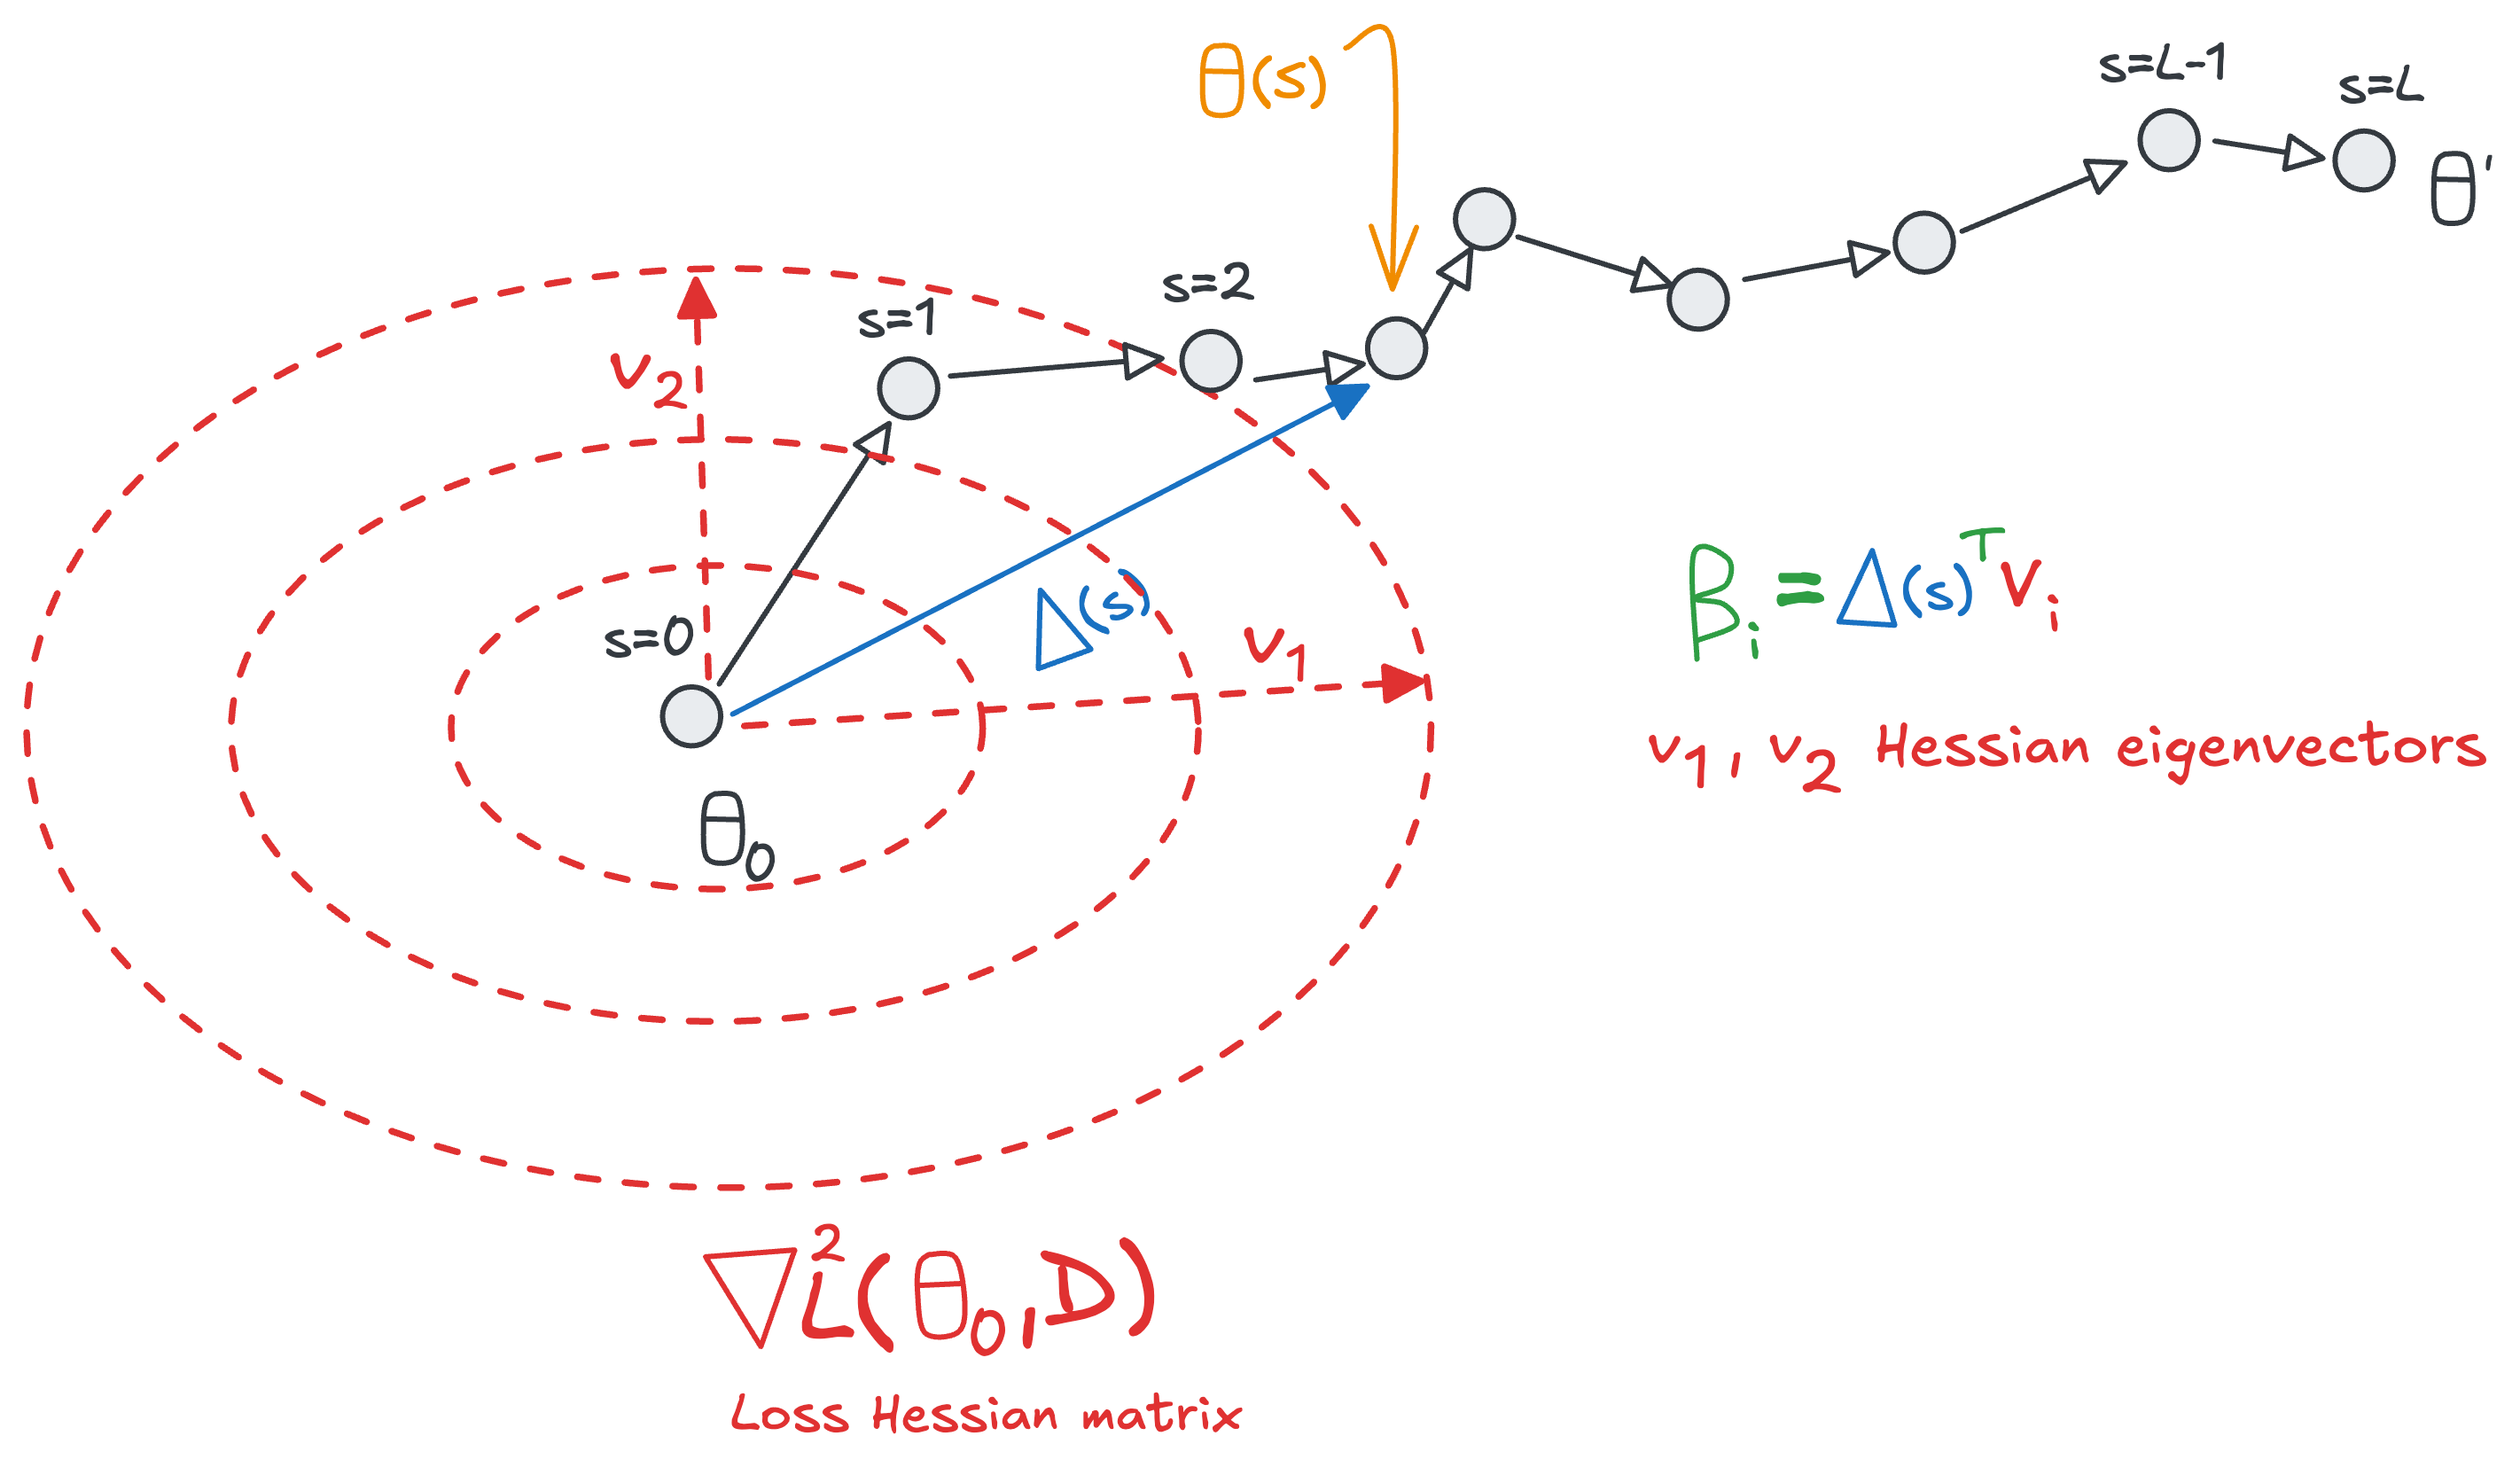
\includegraphics[width=0.8\linewidth]{figures/sketch_dynamics.png}
    \caption{Sketch of the analysis setup.}
    \label{fig:sketch-analysis}
\end{figure}


We want to characterize the dynamics of $\lambda_i(\vparam(s))$ and $ \vDelta(s)^\top \vv_i$. For convenience, we introduce a new set of coordinates for each quantity needed in the analysis, using the Hessian eigen-basis.

\begin{defn}[Coordinates in the Hessian eigenspace: $\alpha, \beta, \gamma$]
\label{def:alpha-beta-gamma}
    Denote by $\{\lambda_1, \dots, \lambda_P\}$, $\{\vv_1, \dots, \vv_P\}$, respectively, the sets of eigenvalues and eigenvectors of the Hessian matrix $\hessian(\vparam_0,\data)$. 
    We define the following quantities: 
    \begin{align}
        &\alpha_i(s) = \vg(s)^\top \vv_i\\
        &\beta_i(s) = \vDelta(s)^\top \vv_i\\
        &\gamma_{ik} = \grad\lambda_k ^\top \vv_i
    \end{align}
    Notice that $\beta(0)=0$ for all $i$.  Further, define the matrix $\Gamma: \Gamma[i,k] = \gamma_{ik}$.
\end{defn}
The matrix $\Gamma$ can be interpreted as the graph of dynamical dependence of the Hessian eigenvectors. If $\gamma_{ik} > 0$ then moving along the $i$-th eigenvector increases the $k$-th eigenvalue. If $\Gamma$ is diagonal the eigenvectors are \emph{dynamically independent}, meaning that the evolution of one is independent of that of another. 


We start characterizing the dynamics of $\beta_i(s)$ by noticing that: 
\begin{align}
    &\beta_i(s+1) = \beta_i(s) + (\vparam(s+1) - \vparam(s))^\top \vv_i = \beta_i(s) + \eta\vg(s)^\top\vv_i\\
    & \beta_i(s+1) - \beta_i(s) = \eta\alpha_i(s) 
\end{align}

To characterize the dynamics of $\lambda_i(\vparam(s))$ we take a first order Taylor expansion around $\lambda_i(\vparam(0)) = \lambda_i$. 
\begin{align}
    &\lambda_i(\vparam(s)) = \lambda_i + \vDelta(s)^\top\grad\lambda_i\\
    &\lambda_i(\vparam(s+1)) - \lambda_i(\vparam(s))  =  (\vparam(s+1) - \vparam(s))^\top\grad\lambda_i\\ 
    & \lambda_i(\vparam(s+1)) - \lambda_i(\vparam(s))  =  \eta \vg(s) \grad\lambda_i 
\end{align}
Moving to continuous time, i.e. taking the limit $\eta \to 0$, for simplicity: 
\begin{align}
    \label{eq:beta-dynamics-implicit}
    & \dot\beta_i(s) = \alpha_i(s) \\
    \label{eq:lambda-dynamics-implicit}
    &\dot\lambda_i(\vparam(s)) = \vg(s)^\top\grad\,\lambda_i = \sum_{k=1}^P \alpha_k(s)\cdot \gamma_{ki}
\end{align}

Approximating $\vg(s)$ using \cref{eq:taylor-3} (see the proof at the end of the section):
\begin{align}
\label{eq:alpha-dynamics}
    &\alpha_i(s) = \alpha_i(0) -  \beta_i(s) \lambda_i   - \frac{1}{2}\sum_{j=1}^P \beta_j^2\gamma_{ij}
\end{align}

The last term appearing in the equations has an important role in the following derivations, and hereafter we call it \emph{Spectrum Instability}. 

\begin{defn}[Spectrum instability]
\label{def:spectrum-instability}
    The spectrum instability at step $s$ along a direction $\vv_i$  is the number 
    \begin{equation}
        \iota_i(s)= \sum_{k=1}^P \beta_k(s)^2 \gamma_{ik}
    \end{equation} 
    The sign of the spectrum instability determines its interpretation: \newline
    "Any update along $\vv_i$  will
    \begin{itemize}
    \item $\iota_i(s)> 0$:  increase the average curvature along the optimization trajectory."
    \item $\iota_i(s) < 0$:  decrease the average curvature along the optimization trajectory."
    \item $\iota_i(s) = 0$:  conserve the  average curvature along the optimization trajectory."
\end{itemize}
    Since $\beta_i(0)=0$ (\cref{def:alpha-beta-gamma}), $\iota_i(0)=0$ for all $i$. 
\end{defn}
In simpler terms, the spectrum instability represents the effect that a movement in the $i$-th eigenvector direction has on the spectrum at time $s$. 

\vspace{0.5cm}


Substituting this definition and \cref{eq:alpha-dynamics} in \cref{eq:beta-dynamics-implicit,eq:lambda-dynamics-implicit}, we obtain the following dynamical system for $s = 0, \dots, L$:
\begin{align}
\begin{cases}
\label{eq:beta-dynamics}
    \dot\beta_i(s) = \alpha_i(0) - \lambda_i \beta_i(s) - \frac{1}{2}\iota_i(s) \\
    \dot\lambda_i(\vparam(s)) = \sum_{k=1}^P \alpha_k(0)\gamma_{ki} - \lambda_k \beta_k(s)\gamma_{ki}  - \frac{1}{2}\iota_k(s)\gamma_{ki}
\end{cases}
\end{align}

with initial conditions $\beta_i(0) = 0$ and $\lambda_i(0) = \lambda_i$. 

In the next section we study the dynamics of $\beta$, as they are independent from the dynamics of $\lambda$ but not viceversa.

\newpage

\textbf{Proof of \Cref{lemma:third-order-spectrum}}
\proof{
For simplicity let us denote $\hessian(\vparam,\data) = \hessian$, $\vV(\vparam) = \vV$ and $\lambda(\vparam) = \lambda$. 
\begin{align}
    &\sum_{i,j,k}\mathcal{T}_{ijk}\cdot (\delta_i\delta_j\delta_k) = \sum_i \delta_i \cdot \partial_{\vparam_i}(\vdelta^\top \hessian \, \vdelta) = \vdelta^\top \grad_{\vparam} \rnd{\vdelta^\top \hessian \, \vdelta}
\end{align}
The quadratic term in parenthesis can be expanded in terms of the eigenvalues of the Hessian matrix as follows: 
\begin{align}
    \vdelta^\top \hessian \, \vdelta = \rnd{\vV \vu}^\top \hessian \rnd{\vV \vu} = \vu^\top \vLambda \vu = \sum_i u_i^2 \lambda_i
\end{align}
Simply noticing that $\vu$ is independent of the parameters and putting everything together gives us the desired result. 
}



\vspace{1cm}

\textbf{Formula for $\vg(s), \alpha(s)$.}
\proof{
    By \cref{eq:taylor-3} we have the following formula for $\loss(\vparam(s), \data)$: 
    \begin{equation}
        \loss(\vparam(s), \data) = \loss(\vparam_0, \data) + a(s) + \frac{1}{2} b(s) + \frac{1}{6} c(s)
    \end{equation}
    Thus the gradient $\grad\loss(\vparam(s), \data)$ with this approximation is: 
    \begin{align}
        \grad\loss(\vparam(s), \data) = \grad a(s) + \frac{1}{2} \grad b(s) + \frac{1}{6} \grad c(s)
    \end{align}
    The gradient of the first 2 terms is readily computed: 
    \begin{align}
        & \grad a(s) = \grad\loss(\vparam_0, \data) \\
        & \grad b(s) = 2\,\hessian(\vparam_0, \data)\,\vDelta(s)
    \end{align}
    Let's now focus on the gradient of the third order term: 
    \begin{align}
        \grad c(s) 
        & = \grad\rnd{\vDelta(s)^\top \rnd{\sum_{i=1}^P (\vDelta(s)^\top\vv_i)^2 \cdot \grad\lambda_i(\vparam_0)}} \\
        & =  \rnd{\grad\vDelta(s)}^\top \rnd{\sum_{i=1}^P (\vDelta(s)^\top\vv_i)^2 \cdot \grad\lambda_i(\vparam_0)} + \vDelta(s)^\top \rnd{\sum_{i=1}^P \grad(\vDelta(s)^\top\vv_i)^2 \cdot \grad\lambda_i(\vparam_0)}\\
        & =  \rnd{\sum_{i=1}^P (\vDelta(s)^\top\vv_i)^2 \cdot \grad\lambda_i(\vparam_0)} + \vDelta(s)^\top \rnd{\sum_{i=1}^P 2\,(\vDelta(s)^\top\vv_i)\cdot \vv_i \cdot \grad\lambda_i(\vparam_0)}\\
        & =  \rnd{\sum_{i=1}^P (\vDelta(s)^\top\vv_i)^2 \cdot \grad\lambda_i(\vparam_0)} + 2\, \rnd{\sum_{i=1}^P  (\vDelta(s)^\top\vv_i)^2 \cdot \grad\lambda_i(\vparam_0)}\\
        & =  3\,\rnd{\sum_{i=1}^P (\vDelta(s)^\top\vv_i)^2 \cdot \grad\lambda_i(\vparam_0)} 
    \end{align}
    By definition $\vg(s) = -\eta\grad\loss(\vparam(s), \data)$ and thus, putting everything together, the formula for $\vg(s)$  is: 
    \begin{align}
        \vg(s) = -\grad\loss(\vparam_0, \data) - \hessian(\vparam_0, \data)\,\vDelta(s) - \frac{1}{2}\rnd{\sum_{i=1}^P (\vDelta(s)^\top\vv_i)^2 \cdot \grad\lambda_i(\vparam_0)} 
    \end{align}
    The definition of $\alpha_i(s)$ is simply $\vg(s)^\top\vv_i$. Thus:
    \begin{align}
        \alpha_i(s) &= -\grad\loss(\vparam_0, \data)^\top\vv_i  -  \vDelta(s)^\top\hessian(\vparam_0, \data)\,\vv_i -\frac{1}{2}\rnd{\sum_{j=1}^P (\vDelta(s)^\top\vv_j)^2 \cdot \grad\lambda_j(\vparam_0)^\top\vv_i} \\
        & = \alpha_i(0) -\rnd{\sum_{j=1}^P (\vDelta(s)^\top\vv_j) \lambda_j \cdot \underbrace{\vv_j^\top \vv_i}_{=0 \text{ for all } i\neq j}} - \frac{1}{2}\rnd{\sum_{j=1}^P (\vDelta(s)^\top\vv_j)^2 \grad\lambda_j(\vparam_0)^\top\vv_i}
    \end{align}
    To get to the final equation simply plugging in the definitions of the Hessian eigenspace coordinates $\beta, \gamma$ (\cref{def:alpha-beta-gamma}):
    \begin{align}
        \alpha_i(s)& = \alpha_i(0) -  \beta_i(s) \lambda_i   - \frac{1}{2}\sum_{j=1}^P \beta_j^2\gamma_{ij}
    \end{align}
}


\newpage

\paragraph{ANALYSIS OF THE DYNAMICS OF $\beta$.}

\Cref{eq:beta-dynamics} describes a coupled non-linear dynamical system. To write the dynamics in a vectorised form, let $\vLambda$ be the diagonal matrix of eigenvalues, and $\valpha(0)$ the vector of constants $\alpha_i(0)$: 
\begin{align}
    \label{eq:vector-beta-dynamics}
    \dot\vbeta = \valpha(0) -  \vLambda \vbeta - \frac{1}{2} \Gamma \vbeta^2
\end{align}
Clearly, the interaction between the individual variables $\beta_i$ is captured by the $\Gamma$ matrix. For a diagonal $\Gamma$, all $\beta_i$ evolve independently. 

\begin{lemma}
    If the eigenvectors of $\hessian(\vparam_0, \data)$ are dynamically independent, i.e. $\gamma_{ik} = \grad\lambda_k^\top\vv_i = 0$ for all $i\neq k$ then the variables $\beta_i$ are independent and $\gamma_{ii} = \|\nabla\lambda_i\|$. The dynamics of $\beta_i$ is then described by the following equation: 
    \begin{equation}
        \label{eq:indepdynamics}
        \dot\beta_i(s) = \alpha_i(0) -\eta \lambda_i \beta_i(s) - \frac{\eta}{2}\beta_i(s)^2 \|\nabla\lambda_i\|
    \end{equation}
\end{lemma}


\begin{figure}[h]
\centering
\begin{tikzpicture}[
    node distance=2cm and 3cm,
    var/.style={circle, draw, minimum size=1cm},
    edge label/.style={draw=none, fill=none, inner sep=1pt},
    >=Stealth
]

% Nodes
\node[var] (b1) at (0,0) {$\beta_1$};
\node[var] (b2) at (3,0) {$\beta_2$};
\node[var] (b3) at (0,-2.5) {$\beta_3$};
\node[var] (b4) at (3,-2.5) {$\beta_4$};

% Edges with weights (labels not styled as nodes)
\draw[->, thick] (b1) -- (b2) node[midway, above, edge label] {$\gamma_{12}$};
\draw[->, thick] (b2) -- (b4) node[midway, right, edge label] {$\gamma_{24}$};
\draw[->, thick] (b3) -- (b1)  node[midway, right, edge label] {$\gamma_{31}$};
\draw[->, thick] (b4) -- (b3) node[midway, above, edge label] {$\gamma_{43}$};
\draw[->, thick] (b1) to[bend right=25] node[midway, left, edge label] {$\gamma_{13}$} (b3);
\draw[->, thick] (b3) to[bend right=25] node[midway, below, edge label] {$\gamma_{34}$} (b4);

\end{tikzpicture}
\caption{The interacting variables can be imagined like a graph. The interaction is given by the gradient descent dynamics. }
\end{figure}

To simplify the analysis we consider two types of nodes, \emph{stable} and \emph{unstable}. The intuition is that for stable nodes the term $\iota_i(s) = (\Gamma\vbeta^2(s))_i < 0$ for all $s$ and viceversa for unstable nodes. 

\begin{defn}[Stable and unstable nodes]
\label{def:stablenodes}
    We say $i$ is an unstable node in the directed graph defined by $\Gamma$ if all the \emph{outgoing} edges have a positive weight, i.e. $\gamma_{ik} > 0$ for all $k$. Similarly, we say is an stable node in the directed graph defined by $\Gamma$ if all the \emph{outgoing} edges have a negative weight, i.e. $\gamma_{ik} < 0$ for all $k$.
 \end{defn}
 \begin{corr}
     If $i$ is an unstable node, then $\iota_i(s)>0$ for all $s \in [L]$. And conversely, if $i$ is a stable node, then $\iota_i(s)<0$ for all $s \in [L]$.
 \end{corr}

The three independent components in \cref{eq:vector-beta-dynamics} encourage three distinct behaviours in $\vDelta(s)$ during optimization, two of which are known: 
\begin{enumerate}
    \item  Alignment with eigenvectors $\vv_i : \alpha_i(0) < 0$ and  negative alignment with $\vv_i : \alpha_i(0) > 0$. 
    \item Alignment with the negative eigenvalues directions, i.e. with $\vv_i : \lambda_i < 0$. 
    \item \emph{Alignment with stable directions, i.e. $\vv_i : \gamma_{ik} < 0 \,\,\forall\;k$.}
\end{enumerate}
These components may interfere with each other, reducing their respective effects. Ultimately, this depends on the spectrum of $\hessian(\vparam_0, \data)$ and the spectrum of $\Gamma$.  The third behaviour is what we call the \emph{spectral stability bias of gradient descent}:
\newpage
\begin{thm}[Spectral Stability Bias of Full-batch Gradient Descent]
    \label{theo:implicit-bias}
    Using the definition of optimization trajectory in \cref{def:opt-traj} and of the $\alpha,\beta, \gamma, \iota$ variables in \cref{def:alpha-beta-gamma,def:spectrum-instability}, the dynamics of $\beta_i(s) = \vDelta(s) ^\top \vv_i$ for all $i$ obey the law: 
    \begin{align}
        &\dot\beta_i(s) = \alpha_i(0) -\lambda_i \beta_i(s) - \frac{1}{2}\iota_i(s),
    \end{align}
    where $\iota(s)$ determines the \emph{stability} of the i-th eigenvector. If $\iota(s) \le 0  \;\forall s$ we call the eigenvector \emph{stable}, as it does not increase the curvature along the optimization trajectory and unstable otherwise. Furthermore, \textbf{if there exist a \emph{stable} direction of non-positive curvature then the update of full-batch gradient descent will align with it}, i.e. $\dot\beta_i(s) > 0$ for all $s$.
\end{thm}

\vspace{1cm}

\subsection{EXAMPLE: LOGISTIC REGRESSION}
\label{subsec:logistic-example}

\begin{center}
\begin{tikzpicture}[
    node distance=0.5cm,
    every node/.style={font=\small, line width=1pt},
    input/.style={circle, draw=black, minimum size=0.8cm},
    hidden/.style={circle, draw=black, minimum size=0.8cm, fill=white},
    output/.style={circle, draw=black, minimum size=0.8cm, align=center},
    weightlabel/.style={font=\scriptsize},
    every path/.style={->, line width=1pt}
  ]

  % Input nodes
  \node[input] (x1) at (0,0) {$x_1$};
  \node[input] (x2) at (1.2,0) {$x_2$};
  \node (dots) at (2,0) {$\cdots$};
  \node[input] (xd) at (3,0) {$x_d$};

  % Hidden node (linear combination output z)
  \node[hidden] (z) at (1.5,1.5) {$z$};

  % Output node (sigma(z))
  \node[output, above=0.5cm of z] (yhat) {$f$};

  % Arrows from inputs to z with weight labels
  \draw[->] (x1) -- (z) node[midway, left, weightlabel] {$w_1$};
  \draw[->] (x2) -- (z) node[midway, left, weightlabel] {$w_2$};
  \draw[->] (xd) -- (z) node[midway, right, weightlabel] {$w_d$};

  % Arrow from z to output
  \draw[->] (z) -- (yhat) node[midway, left, weightlabel] {$\sigma(\cdot)$};

\end{tikzpicture}
\end{center}

Consider a one layer neural network implementing a logistic model of the data. The parameters consist of a single weight vector $\vw \in \mathbb{R}^d$. Thus the total number of parameters in the network is $P=d$, and for consistency we refer to the set of parameters as $\vparam = \vw$. The input $\vx$ is a weight vector in the same space, and the output of the network is a scalar. 

We write the forward pass through the network by defining the logits $z$. 
\begin{align}
    & z = \vw^\top\vx\\
    & f(\vx; \vparam) = \sigma(z)
\end{align}
The output $f(\vx; \vparam)$ can be interpreted as the parameter $\rho(\vx)$ of a Bernoulli distribution defined on the output space $\{0,1\}$. 
The activation function $\sigma$ is the \emph{logistic function}, whose formula, first and second derivatives are: 
\begin{align}
    & \sigma(z) = \frac{1}{1 + \exp(-z)}\\
    & \dot\sigma(z) = \sigma(z)\,(1 - \sigma(z))\\
    & \ddot\sigma(z) = \dot\sigma(z) (1 - 2\sigma(z))
\end{align}
Finally, we define the logistic loss, a binary cross-entropy between the model output distribution and the data. Let $(\vx,y)$ be an input-output pair, then the loss of the network with parameters $\vparam$ is:
\begin{align}
    & \loss(\vparam, (\vx,y)) = -y \log \rnd{f(\vx; \vparam)} + (1-y) \log\rnd{1 - f(\vx; \vparam)}
\end{align}

\paragraph{Gradient and Hessian. }
We compute the gradient $\grad{\loss(\vparam, (\vx,y))}$ with respect to the parameters $\vparam$ using the chain rule: 
\begin{align}
    &\grad{\loss(\vparam, (\vx,y))} = \deriv{\loss(\vparam, (\vx,y))}{z} \cdot \grad{z}\\
    & \deriv{\loss(\vparam, (\vx,y))}{z} = \sigma(z) - y 
    \hspace{1cm}  \grad{z} = \vx
        \\
    & \grad{\loss(\vparam, (\vx,y))} =  (\sigma(z) - y)\cdot \vx  
\end{align}
Similarly, we write the Hessian:
\begin{align}
\label{eq:hessian}
    \hessian(\vparam, (\vx, y)) = 
            \deriv{(\sigma(z) - y)\cdot \vx}{\vw}
    &= \dot\sigma(z)\cdot \vx\vx^\top
\end{align}

\begin{remark}
    \todo{I find this fact quite surprising.} Note that there is no information of the labels in the hessian of this logistic network. Thus the curvature is purely determined by the input. One consequence of this fact is that if the output where to shift (e.g. task shift), the curvature would remain the same. 
\end{remark}

\paragraph{Introducing tasks, and datasets.} Consider a collection of input-output pairs, which we call dataset $\data = \{(\vx_i, y_i)\}_{i=1}^N$. The number of samples if $N$ and $p = P/N$ is the over-parametrization ratio. Given a dataset $\data$, a task is the learning problem of finding a $\vparam \in \mathbb{R}^d$ which best fits the data, according to the logistic loss. Define the average loss across the dataset: 
\begin{align}
    \loss(\vparam, \data) = \langle \loss(\vparam, \cdot) \rangle_{\data} = \frac{1}{N} \sum_{i=1}^N \loss(\vparam, (\vx_i, y_i))
\end{align}
We use the notation $\langle g(\cdot) \rangle_\mathcal{P}$ to denote the expectation of $g(\cdot)$ where its input is sampled from the distribution $\mathcal{P}$. Alternatively, we use the following matrix notation: $\vX$ denotes the $N\times d$ dimensional matrix, where the dataset inputs are stacked row-wise; similarly $\vy$ is the $N$ dimensional vector of dataset outputs; and finally, $\loss(\vparam, (\vX, \vy))=\loss(\vparam, \data)$. 

By the linearity of the derivative operator we have: 
\begin{align}
\label{eq:gradient-batch}
    & \grad\loss(\vparam, (\vX, \vy)) = \frac{1}{N}\,(\sigma(\vz) - \vy)^\top \vX\\
\label{eq:hessian-batch}
    & \hessian(\loss(\vparam, (\vX, \vy))) = \frac{1}{N}\, \cdot \vX^\top\dot\vS \vX,
\end{align}
where we denote by $\dot\vS = \mbox{diag}\rnd{\dot\sigma(\vz)}$ the $N\times N$ diagonal matrix whose entries are the activation derivatives for each input.

\paragraph{Third order Taylor expansion.}
We now write the third-order Taylor expansion of the loss $\loss(\vparam, \data)$ around a point in the parameter space $\vparam_0$: 
\begin{align}
\label{eq:Taylor-general-logistic}
    &\loss(\vparam_0 + \vdelta, \data) - \loss(\vparam_0, \data) = a + \frac{1}{2} b + \frac{1}{6} c
\end{align}
Let's go term by term. For the first-order term, using \cref{eq:gradient-batch}: 
\begin{align}
\label{eq:Taylor-first-logistic}
    & a = \grad\loss(\vparam_0, \data)^\top\vdelta = \frac{1}{N}\,(\sigma(\vz) - \vy)^\top \vX \vdelta
\end{align}
For the second-order term, using \cref{eq:hessian-batch}: 
\begin{align}
\label{eq:Taylor-second-logistic}
    & b = \vdelta^\top\hessian(\vparam_0, \data)\,\vdelta = \vdelta^\top \rnd{\frac{1}{N}\, \cdot \vX^\top  \dot\vS \vX}\,\vdelta
\end{align}
Finally, using \cref{lemma:third-order-spectrum} we can write the third-order term: 
\begin{align}
\label{eq:Taylor-third-logistic}
    c = \sum_{i,j,k}\mathcal{T}_{ijk}\cdot (\delta_i\delta_j\delta_k) = \vdelta^\top \rnd{\sum_{i=1}^P (\vdelta^\top \vv_i)^2 \cdot \grad\,\lambda_i(\vparam)},
\end{align}
where $(\lambda_i, \vv_i)_{i=1}^P$ are the eigenvalue-eigenvector pairs of the Hessian matrix computed in $\vparam_0$. 

\paragraph{Eigendecomposition of the Hessian and Third order term.} 
In order to compute the third order term of the Taylor expansion we look at the eigendecomposition of the Hessian matrix as by \cref{lemma:third-order-spectrum}. 

Let $\vX = \vU \vD \vV^\top $ be the singular value decomposition of $\vX$. Then the product $\vX^\top  \dot\vS \vX$ takes the form $\vV \vD \vU^\top \dot\vS \vU \vD \vV^\top$ and the Hessian: 
\begin{align}
    \hessian(\loss(\vparam, (vX, \vy))) = \frac{1}{N}\, \cdot \rnd{\vV \vD \vU^\top \dot\vS \vU \vD \vV^\top}
\end{align}
This matrix notation is not very enlightening. One special case is when $\dot\sigma(\vz)$ is constant across the inputs $\vz$ and then the Hessian is equivalent to a \emph{rescaled} input covariance, where the scaling factor is $\dot\sigma(\vz)=s$. Another way to write the Hessian is as follows: 
\begin{align}
\label{eq:Hessian}
    \hessian(\loss(\vparam, (\vX, \vy))) = \frac{1}{N}\, \sum_{i=1}^N \dot\sigma(\vz_i) \cdot \vx_i\vx_i^\top
\end{align}
Thus the Hessian can be seen as a weighted average of the individual input covariances, where the weights are given by the model's certainty on the given input.

The third order term in the Taylor expansion can then be written as: 
\begin{align}
\label{eq:Taylor-third-logistic-better}
    c =  \frac{1}{N}\,\vdelta^\top  \rnd{\sum_{i=1}^N\nabla\dot\sigma(\vz_i)\, (\vdelta^\top \vx_i)^2 }
\end{align}
Thus the input vectors define a natural (but not orthonormal and overcomplete) coordinate system for the logistic model: $\beta_i = \vdelta^\top \vx_i$. 
Thus instead of the eigenvalue basis we may use $\vX$ as the basis for our analysis of gradient descent optimization. 

We can further write out $\nabla\dot\sigma(\vz_i)$ using the chaing rule: 
\begin{align}
    \nabla\dot\sigma(\vz_i) = \ddot\sigma(\vz_i)\cdot \nabla\vz = \ddot\sigma(\vz_i)\cdot \vx_i 
\end{align}
Then the third order term in the Taylor expansion becomes:
\begin{align}
    c 
    &=  \frac{1}{N}\, \vdelta^\top  \rnd{\sum_{i=1}^N \ddot\sigma(\vz_i)\cdot \vx_i\, (\vdelta^\top \vx_i)^2 } \\
    &= \frac{1}{N} \,\sum_{i=1}^N\ddot\sigma(\vz_i)\cdot(\vdelta^\top \vx_i)^3
\end{align}

\paragraph{(Intermezzo) The logistic derivatives and model uncertainty.}

Since the derivatives of the logistic function figure prominently in the equations we discuss their interpretation. 
\begin{figure}[h!]
    \centering
    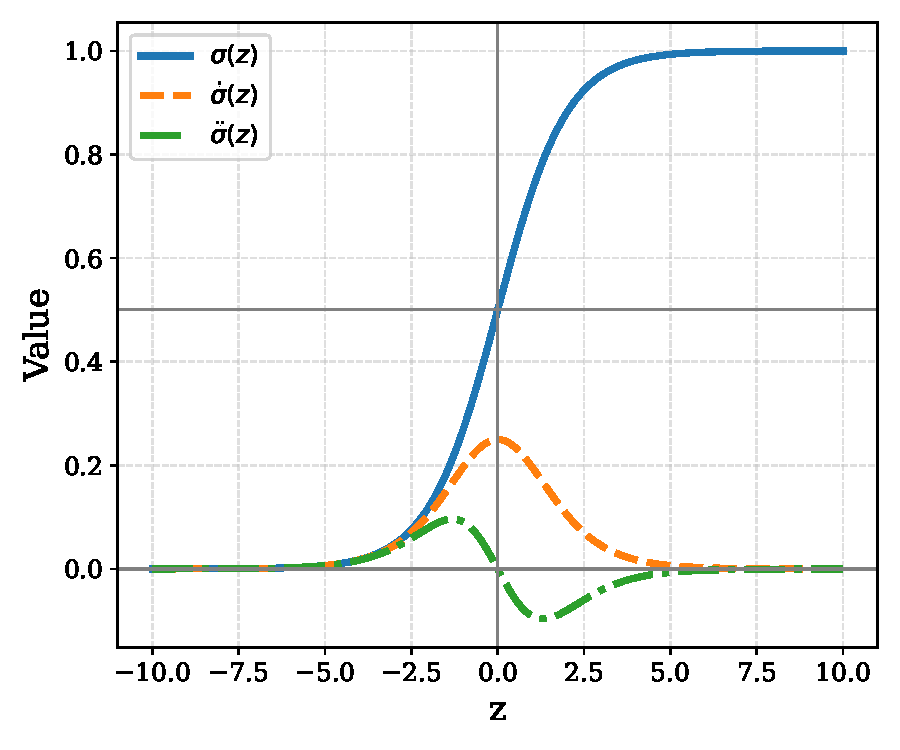
\includegraphics[width=0.3\linewidth]{figures/logistic_wide_range.pdf}
    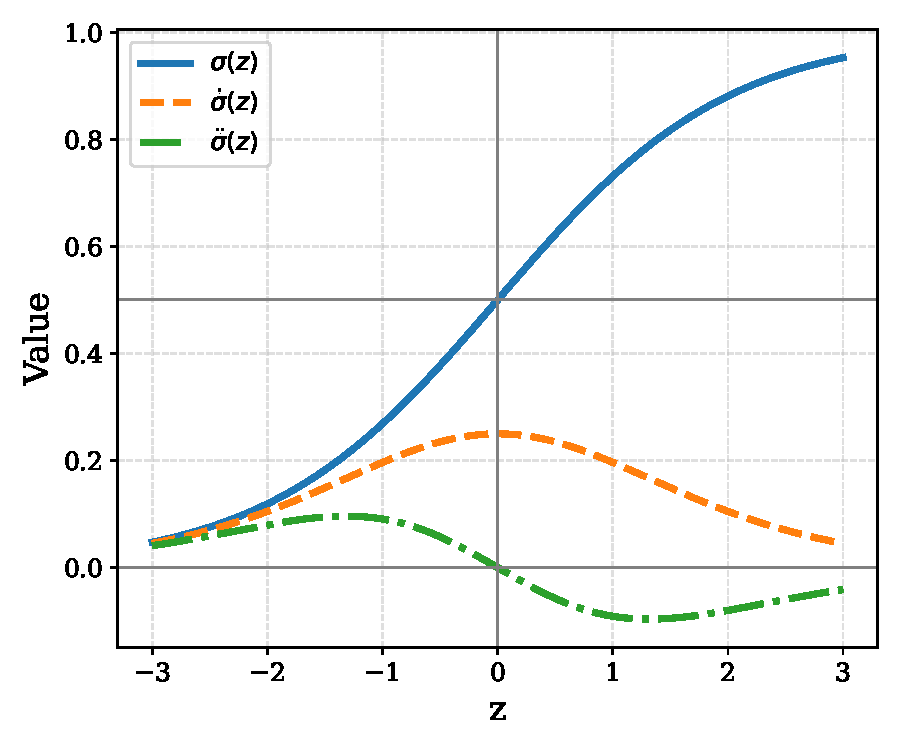
\includegraphics[width=0.3\linewidth]{figures/logistic_zoomed.pdf}
    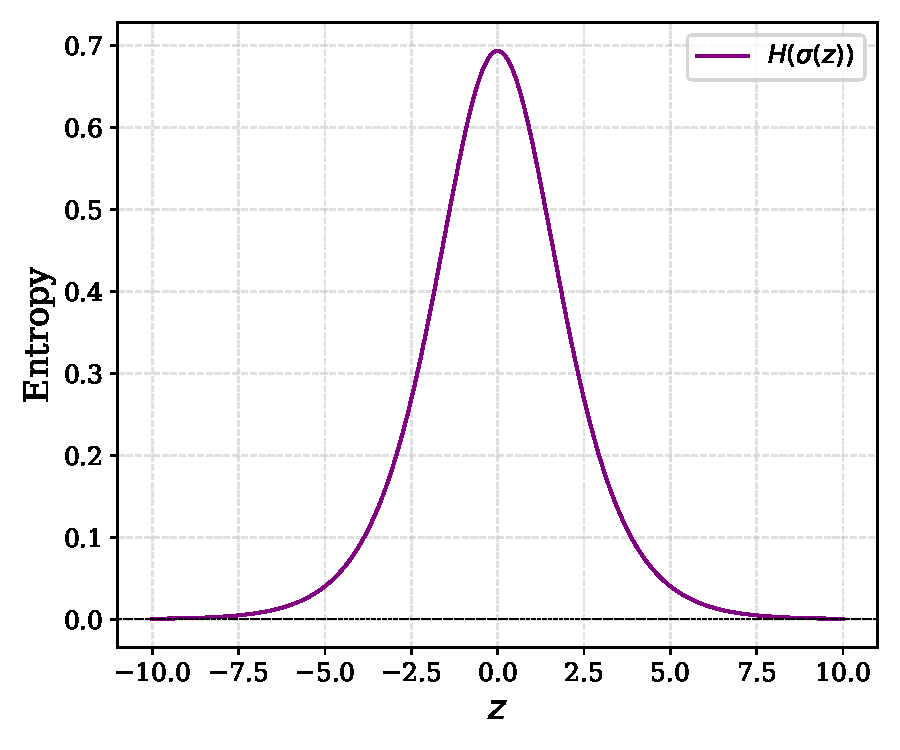
\includegraphics[width=0.3\linewidth]{figures/logistic_entropy.pdf}
    \caption{(First two, starting from the left) Logistic function $\sigma(z)$ and its first and second derivatives. In the middle, a zoomed-in version, with center in $0$. (Rightmost) Entropy of the Bernoulli distribution associated with the parameter $\sigma(z)$, as a function of $z$.}
    \label{fig:logistic-function}
\end{figure}
As we said above, the network output $f(\vx;\vparam) = \sigma(z)$ can be interpreted as the parameter $\rho(\vx)$ of a Bernoulli distribution defined on the output space. In particular, $\lim_{z \to + \infty} \sigma(z) = 1$ and $\lim_{z \to - \infty} \sigma(z) = 0$. Thus, as $z$ grows in magnitude the network prediction is more "certain", as the predictive distribution entropy decreases to $0$. As clearly visible from \cref{fig:logistic-function} the entropy of the respective predictive distribution and the first derivative of the logistic function have similar shapes, peaking at $z=0$ --which corresponds to a uniform distribution-- and exponentially decaying symmetrically away from $0$. Thus in a way we could interpret $\dot \sigma(z)$ as the \emph{uncertainty} in the prediction of the input. The inputs with highest uncertainty will be those closest to the decision boundary --which, in the case of the linear logistic model considered here, is a line in the input space. 

Then what is the interpretation of the second order derivative $\ddot \sigma(z)$, figuring in the third order term of the Taylor expansion? Building on our interpretation of $\dot \sigma(z)$, it is the change in model uncertainty, as $z$ increases. 
\begin{itemize}
    \item $\ddot\sigma(z) > 0$ (for all $z<0$): increasing $z$ increases the predictive uncertainty. 
    \item $\ddot\sigma(z) <0$ (for all $z>0$): increasing $z$ decreases the predictive uncertainty. 
    \item $\ddot\sigma(z) = 0$ (for $z=0$ or $z=\pm \infty$): increasing $z$ has no effect.
\end{itemize}

This interpretation provides a clean link between the geometric characteristics of the loss in the parameter space, and the probabilistic characterization of the network function. In a nutshell, the curvature of the loss in the parameter space --and how it changes as the parameters change-- is directly linked with the uncertainty in the network's predictions: with flatter landscapes corresponding to less uncertainty.

\paragraph{Optimization analysis.}

Similarly to what done for the general case in \cref{subsec:hessian-spectral-stability} let's now analyze the optimization trajectory of gradient descent on the loss as approximated by the third order Taylor expansion (\cref{eq:Taylor-general-logistic,eq:Taylor-first-logistic,eq:Taylor-second-logistic,eq:Taylor-third-logistic-better}). For this, we take $\vparam_0$ to be the initialization, or the starting point of the optimization trajectory $\vparam(0) = \vparam_0$. Now define $\vg(s)$\footnote{$\grad{\loss(\vparam(s),\data)}$ has dimension $1\times d$, but we choose the column vector notation for $\vg(s)$.}: 
\begin{align}
    \vg(s) 
    &= -\grad{\loss(\vparam(s),\data)}^\top \nonumber\\
    &= -\frac{1}{N} \sum_{i=1}^N (\sigma(z^i_0)-y_i) \cdot \vx_i - \frac{1}{N} \sum_{i=1}^N \dot\sigma(z_0^i) (\vDelta(s)^\top \vx_i) \cdot \vx_i - \frac{1}{2N} \sum_{i=1}^N \ddot\sigma(z_0^i)  (\vDelta(s)^\top \vx_i)^2 \cdot \vx_i \nonumber
\end{align}
For notational simplicity we hereafter call $\dot\sigma(z_0^i) = \dot\sigma_i$ and similarly $\ddot\sigma(z_0^i) = \ddot\sigma_i$ and the residuals at initialization as $\ve = \vy - \sigma(\vz_0)$. ecall that $\vDelta(s) = \vparam(s) - \vparam_0 = \vDelta(s-1) + \eta \vg(s)$. Moving to continuous time $t$, by taking the limit $\eta \to 0$, we write $\partial_t\vDelta(t) = \vg(t)$.
\begin{align}
    \partial_t \vDelta(t)  
    &= \frac{1}{N} \sum_{i=1}^N e_i \cdot \vx_i - \frac{1}{N} \sum_{i=1}^N \dot\sigma_i (\vDelta(t)^\top \vx_i) \cdot \vx_i - \frac{1}{2N} \sum_{i=1}^N \ddot\sigma_i  (\vDelta(t)^\top \vx_i)^2 \cdot \vx_i \nonumber \\
\label{eq:dynamics-delta-logistic}
    &= \frac{1}{N} \sum_{i=1}^N \rnd{e_i - \dot\sigma_i (\vDelta(t)^\top \vx_i) - \ddot\sigma_i  (\vDelta(t)^\top \vx_i)^2}\cdot \vx_i
\end{align}
From \cref{eq:dynamics-delta-logistic} we see that the parameters evolution is driven by the input data:  $\partial_t \vDelta(t)= \frac{1}{N} \sum_{i=1}^N \omega_i(t) \cdot \vx_i$ is a weighted sum of the data points, where the weight of a data point is
\begin{equation}
\label{eq:weight-dynamics-delta-datapoint}
    \omega_i(t) = e_i - \dot\sigma_i (\vDelta(t)^\top \vx_i) - \ddot\sigma_i  (\vDelta(t)^\top \vx_i)^2
\end{equation}
\newpage
Thus the impact of any data point on the parameter update is composed of several factors: 
\begin{itemize}
    \item A constant factor depending on the initial prediction error $e_i$; 
    \item A linear term $- \dot\sigma_i (\vDelta(t)^\top \vx_i)$ which decays the weight of \emph{uncertain} prediction points, pushing them towards the decision boundary;
    \item A quadratic term $- \ddot\sigma_i (\vDelta(t)^\top \vx_i)^2$ which decays the weight of points which \emph{increase predictive uncertainty} ($\ddot\sigma(z)>0$), encouraging alignment with points which \emph{decrease predictive uncertainty.}
\end{itemize}

\textcolor{blue}{Ideas from here: 
\begin{itemize}
    \item Study the evolution of the alignment to any individual data point: $\partial_t \vDelta(t)^\top\vx_j = z_j(t) - z_j(0)$
    \item Study the evolution of $\vDelta(t)$ in the eigenspace of the data covariance matrix. Define all the quantities of interest in the coordinate space given by the input covariance. 
\end{itemize}
}


\paragraph{Differences between Second and Third order optimization.}
The optimization analysis above is based on a Taylor expansion of the loss around the initialization point $\vparam_0$, which gives us the gradient formula depending on the first, second and third order terms of the loss (\cref{eq:g(s)-logistic}). This procedure allows us to assess the effect of these terms \emph{in the optimization process}. 

In particular, for Continual Learning (CL), we are interested in understanding the effect of the third (or higher) order terms, since many CL algorithms rely on second-order approximations.

From \cref{eq:dynamics-beta-logistic} and \cref{eq:weight-dynamics-delta-datapoint} we see that the third order term contributes with an additional term $ - \ddot\sigma_i  (\vDelta(t)^\top \vx_i)^2$ (highlighted below) to the weighing of data points in the parameter dynamics. Its effect can be easily interpreted as nudging the update towards data points which \emph{reduce prediction uncertainty}. 

The term introduced by the second order term in the optimization reduces the alignment to data points which are uncertain, thus reducing the prediction error. However, a second order approximation fails to capture the entropy reduction effect, which is implicit in the dynamics.

\begin{align}
    \partial_t \vDelta(t)  
    &= \frac{1}{N} \sum_{i=1}^N \rnd{e_i - \dot\sigma_i (\vDelta(t)^\top \vx_i)  \textcolor{orange}{-\ddot\sigma_i  (\vDelta(t)^\top \vx_i)^2}}\cdot \vx_i
\end{align}

\textcolor{blue}{Next steps: 
\begin{itemize}
    \item Connecting the entropy reduction to forgetting (+ introducing full CL setup)
\end{itemize}
}

\begin{comment}
    
\paragraph{EXAMPLE: 2 LAYER NETWORK}
Let \( x \in \mathbb{R}^d \) be the input, and let the network have a single hidden layer of width \( m \). The parameters are:
\begin{itemize}
    \item First-layer weights: \( W \in \mathbb{R}^{m \times d} \)
    \item Second-layer weights: \( a \in \mathbb{R}^m \)
\end{itemize}

Let \( \sigma: \mathbb{R} \to \mathbb{R} \) be a smooth activation function. The output of the network is:
\[
f(x; \vparam) = \sum_{i=1}^m a_i \sigma(w_i^\top x) = a^\top \sigma(Wx),
\]
where \( w_i \in \mathbb{R}^d \) is the \( i \)-th row of \( W \), and \( \vparam = (a, W) \) denotes all trainable parameters.

Consider the squared loss:
\[
\loss(x, y; \vparam) = \frac{1}{2}(f(x) - y)^2.
\]

Let \( r := f(x) - y \) denote the residual. Then the gradients of the loss are:

\paragraph{With respect to \( a_i \):}
\[
\frac{\partial \mathcal{L}}{\partial a_i} = r \cdot \sigma(w_i^\top x).
\]

\paragraph{With respect to \( w_i \):}
\[
\frac{\partial \mathcal{L}}{\partial w_i} = r \cdot a_i \cdot \sigma'(w_i^\top x) \cdot x \in \mathbb{R}^d.
\]

\subsection*{Hessian}

The Hessian of the loss with respect to the parameters \( \vparam = (a, W) \in \mathbb{R}^{m + md} \) is given by:

\[
\nabla^2_\vparam \mathcal{L} = (\nabla_\vparam f)(\nabla_\vparam f)^\top + r \cdot \nabla_\vparam^2 f.
\]

We write the Hessian in block form:
\[
\nabla^2_\vparam \mathcal{L} =
\begin{bmatrix}
H_{aa} & H_{aW} \\
H_{Wa} & H_{WW}
\end{bmatrix}.
\]

Let \( z_i = w_i^\top x \), \( \sigma_i := \sigma(z_i) \), \( \sigma_i' := \sigma'(z_i) \), and \( \sigma_i'' := \sigma''(z_i) \). Then:

\paragraph{1. \( H_{aa} \in \mathbb{R}^{m \times m} \):}
\[
(H_{aa})_{ij} = \sigma_i \sigma_j.
\]

\paragraph{2. \( H_{aW} \in \mathbb{R}^{m \times md} \):} This is block-diagonal. For \( i = j \),
\[
\frac{\partial^2 \mathcal{L}}{\partial a_i \partial w_j} = \delta_{ij} \cdot \sigma_i' (1 + r) x.
\]

\paragraph{3. \( H_{WW} \in \mathbb{R}^{md \times md} \):} Block \( (i, j) \) is:
\[
\frac{\partial^2 \mathcal{L}}{\partial w_i \partial w_j}
= r \cdot a_i a_j \sigma_i' \sigma_j' x x^\top + \delta_{ij} \cdot a_i \sigma_i'' x x^\top.
\]

\subsection*{Summary}

The full Hessian consists of:
\begin{itemize}
    \item An outer product term from the gradient (Gauss–Newton part),
    \item A curvature term involving \( \sigma'' \) and the residual \( r \),
    \item Cross terms between the \( a_i \) and \( w_i \) parameters that are mostly block-diagonal.
\end{itemize}





% A simple corollary is that the $0$ eigenvalues vary only if $|\alpha_i(0)|>0$. 

% \begin{thm}[Stable nullspace]
%     If $\lambda_i = 0$ and $\alpha_i(0) = 0$ then , by the dynamics described in \cref{theo:implicit-bias}, $\dot\beta_i(0) = 0$ for all $s$, and thus $\beta_i(s) = 0$ for all $s$. As a consequence, $\dot\gamma_i(0) = 0$. 
% \end{thm}
% \proof{
% \todo{Write the proof.}

% }

\end{comment}

\newpage
\subsection{Proofs}
Derivative of the logistic loss with respect to the logits. 
\begin{align}
    \deriv{\loss(\vparam, (\vx,y))}{z} 
    &= \deriv{(-y \log \rnd{\sigma(z)} + (1-y) \log\rnd{1 - \sigma(z)})}{z} \\
    &= -y\deriv{(\log \rnd{\sigma(z)})}{z} + (1-y) \deriv{\log\rnd{1 - \sigma(z)})}{z} \\
    &= -y\frac{1}{\sigma(z)}\deriv{\sigma(z)}{z} + (1-y)\frac{1}{1 - \sigma(z)} \deriv{\rnd{1 - \sigma(z)})}{z} \\
    &= -y\frac{\sigma(z)(1 - \sigma(z))}{\sigma(z)} - (1-y)\frac{\sigma(z)(1 - \sigma(z))}{1 - \sigma(z)} \\
    &= -y(1 - \sigma(z))  - (1-y)\sigma(z)\\
    &= \sigma(z) - y
\end{align}
Second order derivative of the logistic function with respect to the logits: 
\begin{align}
    \ddot\sigma(z) 
    &= \deriv{}{z} \left[ \sigma(z)(1 - \sigma(z)) \right]\\
    &= \dot\sigma(z)(1 - \sigma(z)) - \sigma(z) \cdot \dot\sigma(z)\\
    &= \dot\sigma(z) \left[ (1 - \sigma(z)) - \sigma(z) \right]\\
    &= \dot\sigma(z)(1 - 2\sigma(z))
\end{align}

Fixed points derivations: 

To answer this question, we start by analysing the fixed points of \cref{eq:beta-dynamics}. 
\begin{align}
    & p\,\vK_X\ve - p\,\vK_X \dot\vS \vbeta(t) - \frac{p}{2}\vK_X\ddot\vS \vbeta(t)^2 = 0
    % &= p\,\vK_X \rnd{ \ve - \dot\vS \vbeta(t) - \frac{1}{2} \ddot\vS \vbeta(t)^2}
\end{align}
Assuming that $p > 0$ and $\vK_X$ is invertible, we can  write: 
\begin{align}
    & \ve - \dot\vS \vbeta(t) - \frac{1}{2}\ddot\vS \vbeta(t)^2 = 0
\end{align}
Since all the matrices are diagonal, the data  point equations are decoupled:
\begin{align}
    & e_i - \dot\sigma_i \beta_i(t) - \frac{1}{2}\ddot\sigma_i \beta_i(t)^2 = 0
\end{align}
This is a quadratic equation in $\beta_i$, which has two solutions:
\begin{align}
    \beta_i^\star = \frac{-\dot\sigma_i \pm \sqrt{\dot\sigma_i^2 + 2 \ddot\sigma_i\,e_i}}{\ddot\sigma_i}
\end{align}


Remark 6: 
\begin{align}
    \partial_t \vbeta(t) 
    &= p\,\vU D^2\vU^\top\ve - p\,\vU D^2\vU^\top \dot\vS\vU  \vU^\top\vbeta(t) - \frac{p}{2} \vU D^2\vU^\top\ddot\vS \vU \vU^\top\vbeta(t)^2 
    % &= p\,\vK_X \rnd{ \ve - \dot\vS \vbeta(t) - \frac{1}{2} \ddot\vS \vbeta(t)^2}
\end{align}

Define the input covariance matrix $\vSigma_X = \frac{1}{N} \vX^\top \vX.$ We will analyse the dynamics in the space defined by the input covariance. Recall that $\vX = \vU \vD \vV^\top $ and thus $\vSigma_X = \frac{1}{N}\vV \vD^2 \vV^\top $, i.e. $\vV$ are the eigenvectors and $\frac{1}{N}\vD^2$ the eigenvalues of $\vSigma_X$. We can express all the quantities of interest in the coordinates given by the $\vV$ basis. 

\begin{align}
    &\alpha_i(t) = \vg(t)^\top \vv_i \\
    &\beta_i(t) = \vDelta(t)^\top \vv_i\\
    &\gamma_{ki} = \vx_k^\top \vv_i 
\end{align}



In vector and matrix form:  

\begin{align}
    &\valpha(t) = \vV^\top\vg(t) \\
    &\vbeta(t) = \vV^\top\vDelta(t)\\
    &\Gamma = \vX\vV = \vU \vD
\end{align}



Thus 
\begin{align}
    &\vDelta(t)^\top \vx_i = \sum_{j=1}^P \beta_j(t)\,\gamma_{ij} = \vbeta(t)^\top\Gamma_{i:} \\
    &\vX \vDelta(t) = \Gamma \vbeta(t)
\end{align}

Plugging in the formula for $\vg(t)$: 
\begin{align}
    \alpha_i(t) 
    &= \vg(t)^\top \vv_i\\
    &= \frac{1}{N} \vv_i^\top\vX^\top\ve - \frac{1}{N} \sum_{j=1}^N \dot\sigma(z_0^j) (\vDelta(s)^\top \vx_j) \cdot \vv_i^\top\vx_j - \frac{1}{2N} \sum_{j=1}^N \ddot\sigma(z_0^j)  (\vDelta(s)^\top \vx_j)^2 \cdot \vv_i^\top\vx_j \nonumber\\
    &= \frac{1}{N} \vv_i^\top\vX^\top\ve - \frac{1}{N} \sum_{j=1}^N \dot\sigma(z_0^j) (\vDelta(s)^\top \vx_j) \cdot \gamma_{ji} - \frac{1}{2N} \sum_{j=1}^N \ddot\sigma(z_0^j)  (\vDelta(s)^\top \vx_j)^2 \cdot \gamma_{ji} \nonumber\\
    \valpha(t) 
    &= \frac{1}{N} \vV^\top\vX^\top\ve - \frac{1}{N} \Gamma^\top\dot\vS\vX\vDelta(t)
    - \frac{1}{2N} \Gamma^\top \ddot\vS (\vX\vDelta(t))^2 \nonumber\\
    &= \frac{1}{N} \Gamma^\top\ve - \frac{1}{N} \Gamma^\top\dot\vS\Gamma \vbeta(t)
    - \frac{1}{2N} \Gamma^\top \ddot\vS (\Gamma \vbeta(t))^2 \nonumber\\
\end{align}

\vspace{1cm}

Further, let's define $\beta_i(s) = \vDelta(s)^\top \vx_i$. We have: 
\begin{align}
\label{eq:g(s)-logistic}
    \vg(s) 
    &= \frac{1}{N}\vX^\top\ve - \frac{1}{N} \sum_{i=1}^N \dot\sigma_i \beta_i(s) \cdot \vx_i - \frac{1}{2N} \sum_{i=1}^N \ddot\sigma_i \beta_i(s)^2 \cdot \vx_i \\
    &= \frac{1}{N}\vX^\top\ve - \frac{1}{N}\vX^\top \dot\vS \vbeta(s) - \frac{1}{2N}\vX^\top \ddot\vS \vbeta(s)^2
\end{align}
Recall that $\vDelta(s) = \vparam(s) - \vparam_0 = \vDelta(s-1) + \eta \vg(s)$. Moving to continuous time $t$, by taking the limit $\eta \to 0$, we write $\partial_t\vDelta(t) = \vg(t)$. Thus 
\begin{align}
    \partial_t \vbeta(t) = \partial_t\rnd{\vX \vDelta(t)} = \vX \partial_t\vDelta(t) = \vX \vg(t)
\end{align}
Using \cref{eq:g(s)-logistic} we get a formula for $\partial_t \vbeta(t)$ which depends on the input kernel matrix. For convenience, define $\vK_X = \frac{1}{P} \vX\vX^\top$. 
\begin{align}
\label{eq:dynamics-beta-logistic}
    \partial_t \vbeta(t) 
    &= p\,\vK_X\ve - p\,\vK_X \dot\vS \vbeta(t) - \frac{p}{2}\vK_X\ddot\vS \vbeta(t)^2 
    % &= p\,\vK_X \rnd{ \ve - \dot\vS \vbeta(t) - \frac{1}{2} \ddot\vS \vbeta(t)^2}
\end{align}


\begin{remark}[Interpretation of $\beta_i(t)$.]
\label{remark:interpretation-of-beta}
We defined $\beta_i(t) = \vDelta(t)^\top \vx_i$, i.e. the inner product between the input and the distance traveled in parameter space. In the case of our linear model, $\vparam(t) = \vw(t)$, and $\vparam(t)^\top\vx_i = z_i(t)$. Thus, one interpretation is $\beta_i(t) = (\vparam(t) - \vparam(0))^\top\vx_i = z_i(t) - z_i(0)$, i.e. the increase in the logits since initialization. 
\end{remark}
\begin{remark}[Overparametrization $p$ as time constant.]
    The overparametrization constant $p$ figures in the dynamics expression. In particular, $p$ acts as a time constant, which speeds up or slows down the evolution of $\vbeta$. We could rescale time, absorbing $p$ into a new time constant $\tau = pt$ and write $\partial_\tau \vbeta(\tau)$.
\end{remark}
\begin{remark}[Updates in the data span.]
The data kernel $\vK_X$ multiplies all the element in the dynamics \cref{eq:dynamics-beta-logistic}. If the data kernel is rank deficient, i.e. there are more parameters than data points --\emph{overparametrized regime}--, then the components of $\vbeta(0)$ which are in the null space stay fixed. 
\end{remark}


\begin{remark}[Decoupling in the Kernel space coordinates.]
    \cref{eq:dynamics-beta-logistic} describes a coupled system of equations. If we work in the coordinate space of the kernel eigenvectors $\vU$, the system can be decoupled, up to the first order term. More specifically, recall that $\vX = \vU \vD \vV^\top $ and define $\tilde{\vbeta} = \vU^\top \vbeta$, $\tilde{\vz} = \vU \tilde{\vbeta}(t) $, $\tilde{\ve} = \vU^\top \ve$, and $\tilde{\dot\vS} = \vU^\top \dot\vS \vU$, $\tilde{\ddot\vS} = \vU^\top \ddot\vS \vU$ then:
\begin{align}
    \partial_t \tilde\vbeta(t) = p\vD^2\tilde\ve - p\vD^2 \tilde{\dot\vS} \tilde\vbeta(t) - \frac{p}{2}\vD^2 \tilde{\ddot\vS} \rnd{\vU \tilde{\vbeta}(t)}^2
    % &= p\,\vK_X \rnd{ \ve - \dot\vS \vbeta(t) - \frac{1}{2} \ddot\vS \vbeta(t)^2}
\end{align}
This is similar to the idea of working in the Hessian eigenspace coordinate system described above. 
\end{remark}


By \cref{remark:interpretation-of-beta} if $\lim_{t\to\infty} \beta_i(t) = \pm \infty $ then the network predictions reach minimum entropy, or minimal uncertainty. 
Given \cref{eq:dynamics-beta-logistic}, what can we say about $\beta(t)$ for $t \to \infty$? 




\begin{prop}[Fixed points]
    This is a quadratic equation in $\beta_i$, which has two solutions:
\begin{align}
    \beta_i^\star = \frac{-\dot\sigma_i \pm \sqrt{\dot\sigma_i^2 + 2 \ddot\sigma_i\,e_i}}{\ddot\sigma_i}
\end{align}
\end{prop}




% ----------------------------------------

\newpage

\section{IMPLICATIONS FOR MULTITASK SEQUENTIAL TRAINING}
Now consider the case of sequential multitask learning. Hereafter we use the un-normalized form of the loss for simplicity:
\begin{equation}
    \loss(\vparam, \data_{1:t}) = \loss(\vparam, \data_1) + \dots + \loss(\vparam, \data_t)
\end{equation}
\begin{equation}
    \vparam_t = \mbox{argmin}_{\vparam} \left\{ \loss(\vparam, \data_1) + \dots + \loss(\vparam, \data_t)\right\} 
\end{equation}


\begin{defn}[Local minima strong conditions.]
\label{def:local-minima-strong-conditions}
    We say that $\vparam^\star$ is a local minima of the loss $\loss(\vparam, \data)$ if the following two conditions hold:
    \begin{align}
    \label{eq:opt-condition2}
    &\nabla\loss(\vparam^\star, \data) = 0\\
    \label{eq:opt-condition3}
    &\hessian(\vparam^\star, \data) \succeq 0
\end{align}
\end{defn}
In practice, we can relax the above conditions. 
We start by proving our results using \cref{def:local-minima-strong-conditions}, then we extend them to \cref{def:local-minima-weak-conditions}. 



\begin{assump}[Stable null-space displacement]
\label{assmpt:stable-ns-displacement}
    Let $\vDelta_{t,t+1} = \vparam_{t+1} - \vparam_t$ be the parameter displacement caused by learning task $t+1$. Further, let $\lambda_i(\hessian)$ denote the i$^{th}$ eigenvalue of the matrix $\hessian$.  We say $\vDelta_{t,t+1}$ is a stable null-space displacement if the following conditions are verified: 
    \begin{enumerate}
        \item $\vDelta_{t,t+1}^\top \hessian(\vparam_t, \data_{1:t})\,\vDelta_{t,t+1} = 0$;
        \item $\vDelta_{t,t+1}^\top \grad{\lambda_i(\hessian(\vparam_t, \data_{1:t}))} \le 0 \hspace{0.5cm} \forall \:i$
    \end{enumerate}
\end{assump}


\begin{corr}[Null-space preservation]
\label{corr:null-space-preserv.}
    Consider the line from $\vparam_{t}$ to $\vparam_{t+1}$: $l_{t,t+1}(\kappa) = \kappa\cdot \vparam_{t+1} + (1-\kappa)\cdot \vparam_{t}$, $\kappa \in [0,1]$. If \cref{assmpt:stable-ns-displacement} is satisfied by $\vDelta_{t,t+1} = \vparam_{t+1} - \vparam_t$, then the following condition is also true: 
    \begin{align}
        \vDelta_{t,t+1}^\top \hessian(l_{t,t+1}(\kappa), \data_{1:t})\,\vDelta_{t,t+1} \le \vDelta_{t,t+1}^\top \hessian(\vparam_t, \data_{1:t})\,\vDelta_{t,t+1} = 0
    \end{align}
\end{corr}

\proof{


For simplicity, we will hereafter drop the data dependence and simply use $\hessian(\kappa)$ to refer to $\hessian(l_{t,t+1}(\kappa), \data_{1:t})$. 

\todo{Either include this assumption in the analysis or get rid of it. Maybe one way to get rid of it: instead of talking about eigenvalues, talk about inner products in the Hessian space.}\textcolor{red}{Assume that $\hessian(\kappa)$ and $\hessian(\vparam_t, \data_{1:t})$ commute such that we can write $\hessian(\vparam_t, \data_{1:t}) =  \vV \vLambda \vV^\top$ and $\hessian(\kappa) = \vV \vLambda(\kappa) \vV^\top$.} Then, for each diagonal entry of $ \vLambda(\kappa)$  we have: 
\begin{align}
    \lambda_i(\kappa) 
    &= \lambda_i + \grad\lambda_i(\kappa)^\top(l_{t,t+1}(\kappa) - \vparam_t) \\
    & = \lambda_i + \underbrace{\grad\lambda_i(\kappa)^\top(\kappa\vDelta_{t,t+1})}_{\le 0 \text{ by \cref{assmpt:stable-ns-displacement}}}
\end{align}
Thus $\lambda_i(\kappa) \le \lambda_i$ for all $i \in [1,P]$. The corollary statement follows: 
\begin{align}
    \vDelta_{t,t+1}^\top\hessian(\kappa)\vDelta_{t,t+1} 
    &= \vDelta_{t,t+1}^\top \vLambda \vV^\top\vDelta_{t,t+1} \\
    &= \sum_{i=1}^P (\vv_i^\top \vDelta_{t,t+1})^2 \, \lambda_i(\kappa) \\
    & \le \sum_{i=1}^P (\vv_i^\top \vDelta_{t,t+1})^2 \, \lambda_i = \vDelta_{t,t+1}^\top \hessian(\vparam_t, \data_{1:t})\,\vDelta_{t,t+1}
\end{align}
% Using a first order expansion, we can further characterize $\vLambda(\kappa)$: 
% \begin{equation}
%     \vLambda(\kappa) = \vLambda(0) + \kappa\, \vDelta^\top \grad_{\vparam}\vLambda(0)
% \end{equation}

% Define the quantity $\phi(\kappa) = \vDelta_{t,t+1}^\top \hessian(\kappa)\,\vDelta_{t,t+1}$. By \cref{assmpt:stable-ns-displacement} we know that:
% \begin{align}
%     & \phi(0) = 0 \\
%     & \dot\phi(\kappa) 
%     = \frac{\partial \vDelta_{t,t+1}^\top \hessian(\kappa)\,\vDelta_{t,t+1}}{\partial \kappa}  \\
%     & \hspace{0.5cm} =\vDelta_{t,t+1}^\top \frac{\partial \hessian(\kappa)}{\partial \kappa}\vDelta_{t,t+1} = \\
%     & \hspace{0.5cm} = \vDelta_{t,t+1}^\top \frac{\partial \vV \vLambda(\kappa) \vV^\top}{\partial \kappa}\vDelta_{t,t+1}\\
%     & \hspace{0.5cm} =(\vV^\top\vDelta_{t,t+1})^\top \frac{\partial\vLambda(\kappa)}{\partial \kappa}(\vV^\top\vDelta_{t,t+1}) \\
%     & \hspace{0.5cm} = (\vV^\top\vDelta_{t,t+1})^\top \frac{\partial\vLambda(\kappa)}{\partial l_{t,t+1}(\kappa)}\frac{\partial l_{t,t+1}(\kappa)}{\partial \kappa}(\vV^\top\vDelta_{t,t+1})\\
%     & \hspace{0.5cm} = (\vV^\top\vDelta_{t,t+1})^\top \mbox{diag}()
%     \grad \vLambda(\kappa) \vDelta_{t,t+1} (\vV^\top\vDelta_{t,t+1})
% \end{align}
}

\begin{corr}[Non-increasing gradient alignment]
\label{corr:non-increasing-gradient-alignm.}
    Consider again the line from $\vparam_{t}$ to $\vparam_{t+1}$: $l_{t,t+1}(\kappa) = \kappa\cdot \vparam_{t+1} + (1-\kappa)\cdot \vparam_{t}$, $\kappa \in [0,1]$. If \cref{assmpt:stable-ns-displacement} is satisfied by $\vDelta_{t,t+1} = \vparam_{t+1} - \vparam_t$, and $\vparam_t$ satisfies the local minima conditions \cref{def:local-minima-strong-conditions}, then the following condition is also true: 
    \begin{align}
        \vDelta_{t,t+1}^\top \grad\loss((l_{t,t+1}(\kappa), \data_{1:t}) \le 0
    \end{align}
\end{corr}

\proof{
 We prove this statement by induction. 

 \textit{Base case: $\kappa=0$.} Since by \cref{def:local-minima-strong-conditions}, $\grad\loss((l_{t,t+1}(0), \data_{1:t}) = 0$ the condition is trivially satisfied. 

 \textit{Inductive hypothesis.} Consider two points on the line, separated by an arbitrarily small $\epsilon > 0$: $l_{t,t+1}(\kappa), l_{t,t+1}(\kappa+\epsilon)$. The inductive hypothesis is that $\vDelta_{t,t+1}^\top \grad\loss((l_{t,t+1}(\kappa), \data_{1:t}) \le 0$. 

 \textit{Inductive step.} We now want to show that $\vDelta_{t,t+1}^\top \grad\loss((l_{t,t+1}(\kappa+\epsilon), \data_{1:t}) \le 0$. For $\epsilon\approx 0$: 
 \begin{align}
     \grad\loss((l_{t,t+1}(\kappa+\epsilon), \data_{1:t}) = \grad\loss((l_{t,t+1}(\kappa), \data_{1:t}) +  \hessian(l_{t,t+1}(\kappa), \data_{1:t})(\epsilon\vDelta_{t,t+1})
 \end{align}
 Thus: 
\begin{align}
     &\vDelta_{t,t+1}^\top\grad\loss((l_{t,t+1}(\kappa+\epsilon), \data_{1:t}) = \\
     &= \hspace{0.2cm}\underbrace{\vDelta_{t,t+1}^\top\grad\loss((l_{t,t+1}(\kappa), \data_{1:t})}_{\le 0 \text{ by inductive hypothesis}} +  \underbrace{\vDelta_{t,t+1}^\top\hessian(l_{t,t+1}(\kappa), \data_{1:t})(\epsilon\vDelta_{t,t+1})}_{\le 0 \text{ by \cref{corr:null-space-preserv.}}} \le 0
 \end{align}
}

\begin{defn}[Linear Mode Connectivity (LMC)]
\label{def:LMC}
    Let $\vparam_1, \vparam_2$ be two points in the parameter space, and define the linear interpolation function $l_{12}(\kappa) = \kappa\cdot \vparam_{2} + (1-\kappa)\cdot \vparam_{1}$. Given a loss function $\loss(\vparam, \data)$ we say that there is Linear Mode Connectivity from $\vparam_{1}$ to $\vparam_{2}$ if the loss is \emph{non-increasing over the curve $\{l_{12}(\kappa),\, \kappa \in [0,1]\}$}:
\begin{align}
    \deriv{\loss(l_{12}(\kappa), \data)}{\kappa} \le 0 \hspace{1cm}\forall \:\kappa \in [0,1]
\end{align}
\end{defn}


\begin{thm}[Linear Multitask Mode Connectivity for stable null-space updates]
    \label{theorem:multitask-mode-connectivity}
    Consider again the line from $\vparam_{t}$ to $\vparam_{t+1}$: $l_{t,t+1}(\kappa) = \kappa\cdot \vparam_{t+1} + (1-\kappa)\cdot \vparam_{t}$, $\kappa \in [0,1]$. If \cref{assmpt:stable-ns-displacement} is satisfied by $\vDelta_{t,t+1} = \vparam_{t+1} - \vparam_t$, and $\vparam_t$ satisfies the local minima conditions \cref{def:local-minima-strong-conditions}, then there is Linear Mode Connectivity (\cref{def:LMC}) from $\vparam_{t}$ to $\vparam_{t+1}$ of the multitask loss $\loss(\cdot, \data_{1:t})$.
\end{thm}

\proof{
% Simply put together \cref{corr:null-space-preserv.,corr:non-increasing-gradient-alignm.}
By the chain rule: 
\begin{align}
    \deriv{\loss(l_{12}(\kappa), \data_{1:t})}{\kappa} 
    & = \deriv{\loss(l_{12}(\kappa), \dataa_{1:t})}{(\vparam_t + \kappa\vDelta_{t,t+1})} \cdot \deriv{(\vparam_t + \kappa\vDelta_{t,t+1})}{\kappa} \\
    & = \grad\loss(l_{12}(\kappa), \data_{1:t})^\top \vDelta_{t,t+1} \le 0 \hspace{0.2cm}\text{ by \cref{corr:non-increasing-gradient-alignm.}}
\end{align}
}



\begin{corr}[Compositionality of stable null-space displacements]
\label{corr:compositionality-of-stable-null-space-displacements}
    Let $\vDelta_{t,t+1} = \vparam_{t+1} - \vparam_t$ be the parameter displacement caused by learning task $t+1$, and similarly $\vDelta_{t+1,t+2} = \vparam_{t+2} - \vparam_{t+1}$. If $\vDelta_{t+1,t+2}$ and $\vDelta_{t,t+1}$ are both stable null-space displacements, respectively for $\loss(\vparam, \data_{1:t})$ and $\loss(\vparam, \data_{1:t+1})$, then also the  vector $\vDelta_{t,t+2} = \vDelta_{t,t+1} + \vDelta_{t+1,t+2} =  \vparam_{t+2} - \vparam_t$ is a stable null-space displacement for the loss $\loss(\vparam, \data_{1:t})$.
\end{corr}

\proof{
We first want to show that:
\begin{align}
    \vDelta_{t,t+2}^\top \hessian(\vparam_t, \data_{1:t}) \vDelta_{t,t+2} = (\vDelta_{t,t+1} + \vDelta_{t+1,t+2})^\top \hessian(\vparam_t, \data_{1:t})\,(\vDelta_{t,t+1} + \vDelta_{t+1,t+2}) = 0
\end{align}
Since, by \cref{assmpt:stable-ns-displacement},  $\vDelta_{t,t+1}^\top \hessian(\vparam_t, \data_{1:t}) \vDelta_{t,t+1} = 0$, then, to prove this first statement, it is sufficient to show that $\vDelta_{t+1,t+2}^\top \hessian(\vparam_t, \data_{1:t}) \vDelta_{t+1,t+2} = 0$. 
By \cref{assmpt:stable-ns-displacement} we also know that:
\begin{align}
    &\vDelta_{t+1,t+2}^\top\hessian(\vparam_{t+1}, \data_{1:t+1}) \vDelta_{t+1,t+2} = 0 \\
    &\vDelta_{t+1,t+2}^\top(\hessian(\vparam_{t+1}, \data_{1:t}) + \hessian(\vparam_{t+1}, \data_{t+1})) \vDelta_{t+1,t+2} = 0
\end{align}
Since $\vparam_{t+1}$ is a minimum of $\loss($
\textcolor{red}{TBC...}



The second statement which we want to show is:
\begin{align}
    \vDelta_{t,t+2}^\top \grad{\lambda_i(\hessian(\vparam_t, \data_{1:t}))} =  (\vDelta_{t,t+1} + \vDelta_{t+1,t+2})^\top \grad{\lambda_i(\hessian(\vparam_t, \data_{1:t}))}\le 0 
\end{align}
\textcolor{red}{TBC...}

}

\begin{thm}[Complete Linear Multitask Mode Connectivity for stable null-space updates]
    \label{theorem:complete-multitask-mode-connectivity}
    Consider the sequence of local minima (\cref{def:local-minima-strong-conditions}) $\vparam_1, \dots, \vparam_T$ generated by a sequential multitask learning algorithm and the corresponding task displacement vectors $\vDelta_2, \dots, \vDelta_T$. If all the task displacement vectors satisfy conditions of \cref{assmpt:stable-ns-displacement} then, for any two task indices $t_1 < t_2$ there is LMC from $\vparam_{t_1}$ to $\vparam_{t_2}$ on the loss $\loss(\vparam, \data_{1:t_1})$.  
\end{thm}


\todo{Weak and strong multitask linear mode connectivity. + corollary that shows from weak to strong by induction}


\vspace{2cm}

\todo{Handle different definition of local minima.}
\begin{defn}[Local minima weak conditions.]
\label{def:local-minima-weak-conditions}
    We say that $\vparam^\star$ is a local minima of the loss $\loss(\vparam, \data)$ if, for some $\epsilon, \delta > 0 $ and $\epsilon, \delta \approx 0$ the following two weak conditions hold:
    \begin{align}
    \label{eq:opt-weak-condition2}
    &\|\nabla_{\vparam}\loss(\vparam^\star, \data)\| = \epsilon\\
    \label{eq:opt-weak-condition3}
    &\hessian(\vparam^\star, \data) \succeq - \delta
\end{align}
\end{defn}


\newpage
\section{IMPLICATIONS FOR CONTINUAL LEARNING}

\giulia{This section needs re-writing}

\subsection{Introducing mixed approximations.}

Let's go back to the multi-task loss $\loss({\vparam, \data_{1:t}})$ (\cref{eq:multi-task-objective}). A data-based approximation of the loss is a function of a data subset $\memory_{1:t} \subset \data_{1:t}$ and we simply denote it by $\hat{\loss}({\vparam, \memory_{1:t}})$. More explicitly, we assume the following form\footnote{This form and the one used for parameter-based approximations is typical in the literature as argued in \cref{sec:introduction}.}: 
\begin{equation}
\label{eq:data-based-approx}
    \hat{\loss}({\vparam, \memory_{1:t}}) = \frac{1}{t}\rnd{{\loss}({\vparam, \memory_{1}}) + \dots + {\loss}({\vparam, \memory_{t}})}
\end{equation}
Thus, the error of a data-based approximation is a function of the set of \emph{absent} memories $\absent_{i:t} = \data_{1:t}\setminus\memory_{1:t}$. If the loss function $\loss$ is additive in its second argument then: 
\begin{equation}
    e(\vparam, \absent_{i:t}) = \loss({\vparam, \data_{1:t}}) - \hat{\loss}({\vparam, \memory_{1:t}}) = \frac{1}{t}\rnd{{\loss}({\vparam, \absent_{1}}) + \dots + {\loss}({\vparam, \absent_{t}})}
\end{equation}
Notice that since the loss is a non-negative function $e(\vparam, \absent_{i:t}) \ge 0$ for all $\vparam$. However, for gradient-based optimization processes, we are not interested in terms of $e(\vparam, \absent_{i:t})$ which are constant in $\vparam$, as they do not influence the optimization process. Therefore, we take a Taylor expansion of the error around a generic $\vparam_0$ for small displacements $\vdelta$: 
\begin{equation}
\label{eq:approximate-error}
    \tilde{e}(\vdelta, \absent_{i:t}) = C_0 + \vg_0^\top \vdelta + \frac{1}{2}\vdelta^\top \hessian(\vparam_0, \absent_{i:t})\vdelta + \mathcal{O}(\|\vdelta\|^3),
\end{equation}
where $C_0 = {e}(\vparam_0, \absent_{i:t})$ is the said constant, $\vg_0 = \nabla_{\vparam}{e}(\vparam_0, \absent_{i:t})$ and $\mathcal{O}(\|\vdelta\|^3)$ hides the higher order terms in the expansion. 

Let's now turn to parameter-based approximations. Hereafter we assume the second-order form: 
\begin{equation}
\label{eq:second-order-approx}
    Q({\vparam;  a, \vb, \vC}) = a + \vb^\top\vparam + \frac{1}{2}\vparam^\top\mbox{\vC}\,\vparam
\end{equation}
In order to quantify the error of this approximation consider again Taylor expansion of the loss around a generic $\vparam_0$ for small displacements $\vdelta$. The error is: 
\begin{equation}
    \tilde{e}(\vparam;  a, \vb, \vC) = (\loss(\vparam_0, \data_{1:t}) - a) + (\nabla_{\vparam}\loss(\vparam_0, \data_{1:t}) - \vb)^\top\vdelta + \frac{1}{2}\vdelta^\top \rnd{\hessian(\vparam_0, \data_{1:t}) - \vC}\,\vdelta
\end{equation}
Again, for optimization purposes, the constants in the approximation error can be discarded. Therefore, for a good approximation it is sufficient to take $\vb = \nabla_{\vparam}\loss(\vparam_0, \data_{1:t})$ and $\vC = \hessian(\vparam_0, \data_{1:t})$, when $\|\vdelta\|^3 \approx 0$.  Typically, regularization methods take $\vb = 0$. This works when either (1)  $\nabla_{\vparam}\loss(\vparam_0, \data_{1:t}) = 0$, i.e. $\vparam_0$ is a local minimum of the loss function, or (2) the displacement vector $\vdelta \perp \nabla_{\vparam}\loss(\vparam_0, \data_{1:t})$, such that the inner-product is $0$. 

Using the two approximations together, we obtain a mixed approximation, which takes the form:
\begin{equation}
    \hat{\loss}(\vparam, \memory_{1:t};a, \vb, \vC) = \hat{\loss}({\vparam, \memory_{1:t}}) + Q({\vparam;  a, \vb, \vC})
\end{equation}
Using the same Taylor expansion of the loss as before, the error of a mixed approximation is: 
\begin{equation}
    \tilde{e}(\vparam; \absent_{1:t}; a, \vb, \vC) = (C_0-a) + (\vg_0-\vb)^\top \vdelta + \frac{1}{2}\vdelta^\top \rnd{\hessian(\vparam_0, \absent_{i:t})-\vC}\vdelta + \mathcal{O}(\|\vdelta\|^3)
\end{equation}
The first-order optimization processed is preserved by the approximation if $\nabla_{\vparam}\tilde{e}(\vparam; \absent_{1:t}; a, \vb, \vC) = 0$, which we translate in two --dependent-- conditions:
\begin{align}
\label{eq:conditions-1}
    &(\vg_0-\vb)^\top \vdelta = 0\\
\label{eq:conditions-2}
    &\vdelta^\top \rnd{\hessian(\vparam_0, \absent_{i:t})-\vC}\vdelta = 0
\end{align}

\giulia{Thoughts. Why using mixed approximations? To spare on the memory cost of replay, by using a fixed-memory quadratic approximation. Thus, the quadratic approximation should capture most of the curvature information of the loss, and replay samples should be used to capture the remaining part. Basically replay should be used to approximate the error of the quadratic approximation. To proceed, we need to understand better what replay does.}

\newpage

What follows in the next pages needs to be rewritten
\newpage
\section{Introduction (high level)}
\label{sec:introduction}
Continual learning is the problem of fitting a model on data which can only be accessed \emph{sequentially}. This study focuses on the typical case where the \emph{data stream} is organized into consecutive subsets of i.i.d. samples, also called \emph{tasks}. Hereafter, we take $T$ to be the total number of tasks, and $t$ to refer to the task which is current to the algorithm. We denote by $\calT_i$ the $i^{th}$ task in the sequence, and by $\data_i$ the training dataset of the task. Finally, we use $\vparam$ to denote the vectorized parameters of the neural network. 

The performance of the network on the task is quantified by a loss function $\ell(\vparam, \data) \in \real^+$: low loss corresponds to high performance. In the context of this study we take the goal of a continual learning to be \emph{to minimize the multi-task loss}, i.e. perform well on all the tasks. Formally, we can write the objective as follows: 
\begin{equation}
\label{eq:multi-task-objective}
    \vparam_t = \mbox{argmin}_{\vparam} \left\{ \loss(\vparam, \data_1) + \dots + \loss(\vparam, \data_t)\right\} 
\end{equation}
Hereafter we refer to this objective as the multi-task objective, and use the shorthand form $\loss(\vparam, \data_{1:t})$ for the multi-task loss. Since the data is only accessed in a sequential fashion, the multi-task objective cannot be directly evaluated by the algorithm, which must instead resort to approximations thereof. Depending on the information used in the approximation, continual learning algorithms can be broadly classified into two separate families\footnote{This is mostly a personal opinion, which I can argue for formally. But I can find some references to back it up.}, which we hereafter call \emph{data-based} and \emph{parameter-based} approximations. 

\paragraph{Data-based approximations.} 
\todo{Introduce distribution-based definition.} Data-based approximations use samples from past tasks to approximate the multi-task loss. The simplest --and still among the most effective \citep{buzzega_rethinking_2021} -- form of data-based approximations is \emph{Experience Replay}, which stores a set $\memory_i$ of $M$ data points from each dataset $\data_i$, and simply replaces $\loss(\vparam, \data_i)$ in \cref{eq:multi-task-objective} with $\loss(\vparam, \memory_i)$. Several more sophisticated approximations have been developed, for example, storing data in the representation space \citep{rebuffi_icarl_2017}, learning a generative model of the past tasks data \citep{shin_continual_2017,van_de_ven_generative_2018}, optimizing the selection of the samples $\memory_i$ to reduce $M$ without compromising on performance \citep{yoon_online_2021}, and many more.  

\paragraph{Parameter-based approximations.}
Parameter-based approximations use information regarding the loss landscape in parameter space to approximate the multi-task loss. One way to do this is by avoiding or penalizing motion along directions of (locally) high curvature of the loss, which correspond to the eigenvectors of the range loss Hessian subspace. Formally, one considers the second order Taylor expansion of the loss around some point $\vparam_0$, approximating 
\begin{equation}
\label{eq:second-order-approx}
    \loss(\vparam, \data_i) \approx \loss(\vparam_0, \data_i) + (\vparam - \vparam_0)^\top\grad_{\vparam}\loss(\vparam_0, \data_i) + (\vparam - \vparam_0)^\top\hessian(\vparam_0, \data_i)(\vparam - \vparam_0),
\end{equation}
where $\hessian(\vparam_0, \data_i)$ represents the Hessian calculated at the point $\vparam_0$. Many algorithms using second-order regularization can be reduced to \cref{eq:second-order-approx} \citep{yin_optimization_2020}. A chief example is  Elastic Weight Consolidation (or EWC) \citep{kirkpatrick_overcoming_2017}, which stores the diagonal of the \emph{Fisher Information matrix} (FIM)\footnote{$F(\vparam, \data_i) = \mathbb{E}_{(x, y) \sim \data_i} \nabla_{\vparam} \log p(y \mid x; \vparam) 
\nabla_{\vparam} \log p(y \mid x; \vparam)^\top 
$} of each task, typically aggregating all the past tasks' matrices with an average. The algorithm penalizes the displacement of parameters with a high Fisher score, by adding to the current task loss the regularizer $\reg(\vparam) = \|\vparam\|_{F_i}^2$. The FIM is equivalent to the Hessian close to a minimum, and therefore EWC can be interpreted as replacing $\hessian(\vparam_0, \data_i)$ in \cref{eq:second-order-approx} by $\Diag(F(\vparam_0, \data_i))$ with $\vparam_0$ being (close to) a minimum of the loss of task $i$. The diagonal approximation is taken to reduce the computational costs of the method, at the expenses of precision. Another way to approximate the multi-task loss by using parameters, is to \emph{isolate} the tasks in separate subsets of the parameter space. This is done either by (1) assigning new parameters to the new task \citep{rusu_progressive_2016,schwarz_progress_2018} or by (2) masking away parameters which have been used to fit the previous tasks\footnote{Methods enforcing sparse updates can be interpreted as a form of parameter isolation.} \citep{mallya_packnet_2018}. These algorithms are also known as \emph{parameter isolation methods} in the literature. Clearly, if there is no change in the parameters which contribute to the previous tasks' function, the performance remains unchanged as new tasks are processed. 

\paragraph{Pros \& Cons of data-based and parameter-based approximations.} An important factor in continual learning is the size of the storage utilized by the algorithm, or equivalently the amount of overhead computation required to learn the tasks sequentially rather than jointly. The overhead should grow as \emph{slowly} as possible in the number of tasks, in order to allow the algorithm to process more tasks within a given fixed computational budget. The main drawback of data-based approximations is that their computational overhead grows linearly in the number of tasks, limiting the applicability of such algorithms in the wild. Parameter-based approximations which rely on regularization can have lower computational overhead (for instance EWC has a constant overhead in the task size), however this gain in computational cost comes at the expenses of performance, which is typically low. On the other hand, parameter-based approximations relying on parameter isolation typically have an overhead growing linearly with the number of tasks (as the number of parameters is linear in the number of tasks), but they guarantee a constant performance on the old tasks. In general, across the literature we observe that multi-task performance and efficiency are in opposition, and increasing one always comes at the expenses of the other \citep{de_lange_continual_2022}. 

\begin{table}[h]
\centering
\caption{Comparison of continual learning approaches. $T$ denotes the number of tasks.}
\label{tab:cl_overhead}
\begin{tabular}{lcc}
\toprule
\textbf{Approach} & \textbf{Computational Overhead} & \textbf{Performance on Old Tasks} \\
\midrule
Data-based & $\mathcal{O}(T)$ & High (Dynamic)\\
Parameter-based (regularization) & $\mathcal{O}(1)$ & Low \\
Parameter-based (isolation) & $\mathcal{O}(T)$ & High (Constant) \\
\bottomrule
\end{tabular}
\end{table}

\section{Connection to a unified Bayesian view of Continual Learning}

\citet{farquhar_unifying_2019}

Geometric intuition ...

\newpage
\section{Motivation and Goals of this study}

A high level introduction is given in \cref{sec:introduction}.
\citet{mirzadeh_linear_2020-1} point out an interesting property of the multi-task objective (\cref{eq:multi-task-objective}). In particular, they demonstrate empirically \emph{Linear Mode Connectivity}\footnote{Simply called Linear Mode Connectivity in the original paper, but we rename it here to distinguish it from the single-task case.} (LMC) between the sequence of multi-task objective minima. More precisely, on a linear path $\vparam_{t_1} \ra \vparam_{t_2}$, with $t_2 > t_1$, the loss of task $t_1$ is not increasing. Additionally, they show that LMC does not hold between the sequence of minima obtained by optimizing the individual tasks' losses consequently --without resetting. This result is not trivial, as, when minimizing the average loss the increase in an individual task's loss might be compensated by the decrease in another task's loss.  In other words, the addition of a task loss restricts the parameter updates to the subspace of low curvature of that loss. 

% There are several questions which are not addressed in \citet{mirzadeh_linear_2020-1}: 
% \squishlist
%     \item How much of the previous tasks data is needed to obtain LMC? The experiments in  \citet{mirzadeh_linear_2020-1} compute the old tasks loss on the full dataset. 
%     \item For how long does the old tasks loss must be added to the current task objective? \todo{Try interleaved replay} The experiments in  \citet{mirzadeh_linear_2020-1} always consider all the old tasks. Does LMC hold even when considering only the last $k$ tasks? 
%     \item How and how much does the geometry of an old task loss change as more tasks are processed?
% \squishend

The results of \citet{mirzadeh_linear_2020-1} suggest that the multi-task objective consolidates the geometry of the old tasks losses by restricting the optimization process to an area of low-loss. In this study we aim to explore further this consolidation process\todo{"Memory consolidation" could be a name}, with the final goal of exploiting it to reduce a data-based approximation to a more efficient parameter-based approximation without sacrificing performance. The goals of the study are presented in more detail in \cref{sec:RQ}. 


\vspace{1cm}


\section{Initial Emprical results} 


\paragraph{Experimental setup}
We train a ResNet-18 network (with Batch Norm, Standard Parametrization) on 10 consecutive image classification tasks, obtained by splitting the 100 classes of CIFAR-100 in 10 sets. The network is optimized with SGD and the learning rate is annealed with cosine scheduling, starting from $0.05$. The network is trained with a multi-head configuration, i.e. separating the outputs of the different tasks\footnote{This scenario is commonly known as \emph{Task-incremental learning}.}. The experiments are organized in three parts: first, we replicate the results of \citet{mirzadeh_linear_2020-1}; then we ablate the amount of data needed from the old tasks in order to obtain LMC; finally we ablate the number of repetitions of a task needed to obtain LMC. 

\paragraph{Replicating consolidation.} We compare the multi-task and single-task objectives solutions. 
\begin{figure}[h!]
    \centering
    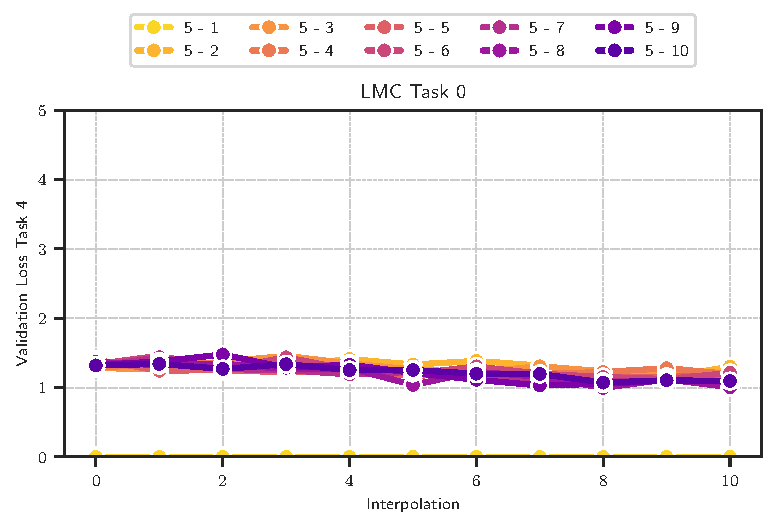
\includegraphics[width=0.45\linewidth]{figures/LMC_task_0.pdf}
    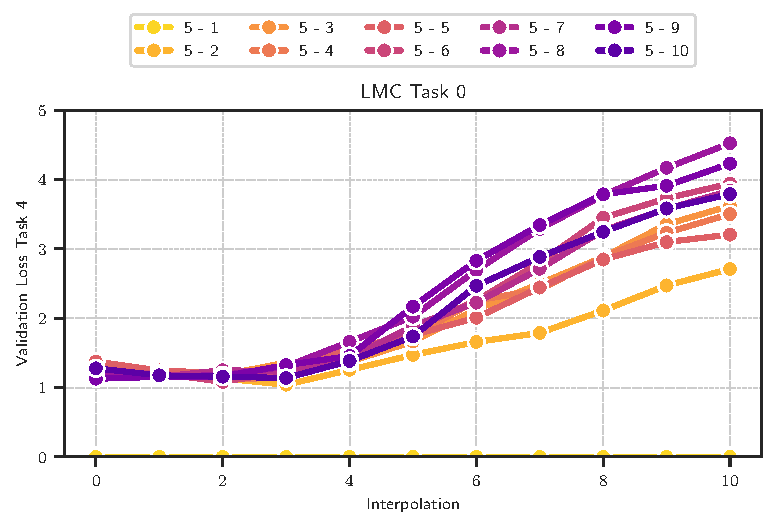
\includegraphics[width=0.45\linewidth]{figures/LMC_task_0_ST.pdf}
    \caption{Comparison of Linear Mode Connectivity between the first task and all subsequent ones in multi-task training (left) and single-task training (right). \textcolor{lightred}{ Attention: labelling in the figure is off: it should be 1-1, 1-2, \dots etc.. The loss is of the first task.}}
    \label{fig:LMC-MTST}
\end{figure}
Our results confirm that there is LMC between the multi-task minima, but not between single-task minima. \cref{fig:LMC-MTST} depicts the (validation) loss on a linear path between the first task solution and all the subsequent ones. Similar patters are observed for later tasks.  

\paragraph{Ablation \#1: amount of data.} In this experiment we evaluate LMC while varying the amount of old tasks' data used in the multi-task loss. More specifically, we keep by sampling with uniform probability a fraction $r$ of the original dataset. In practice, this is equivalent to using the most naive variant of Experience Replay. We take $r=0.5, 0.1, 0.01$. 
\begin{figure}[h!]
    \centering
    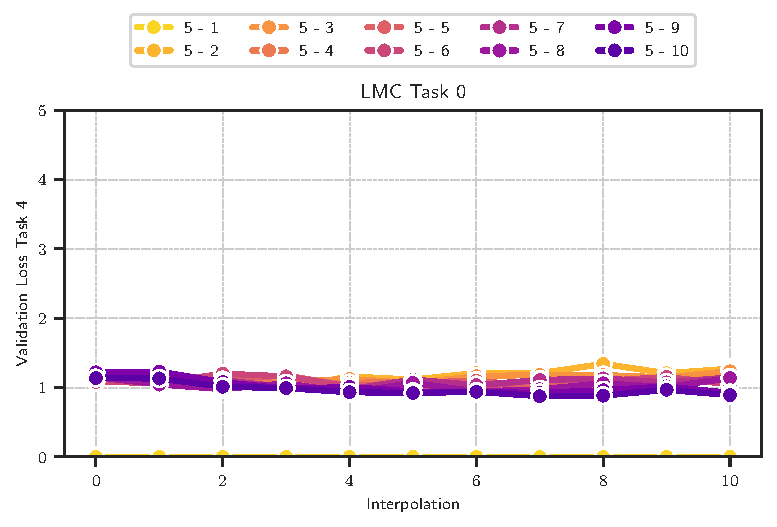
\includegraphics[width=0.3\linewidth]{figures/LMC_task_0_re05.pdf}
    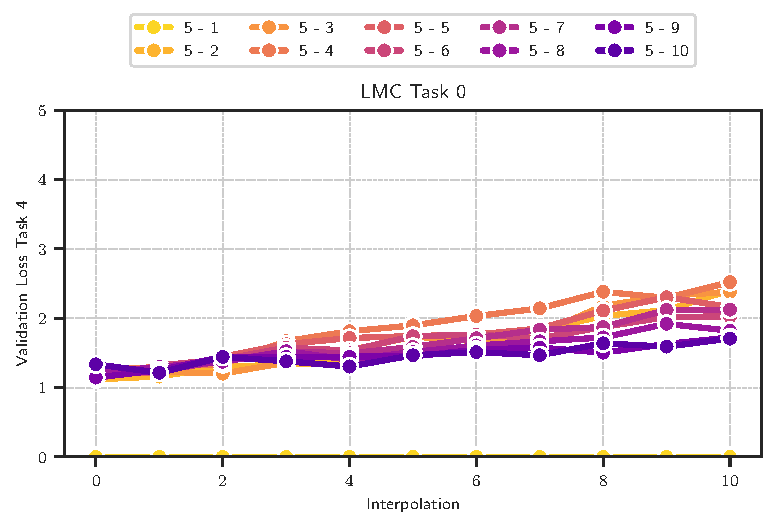
\includegraphics[width=0.3\linewidth]{figures/LMC_task_0_re01.pdf}
    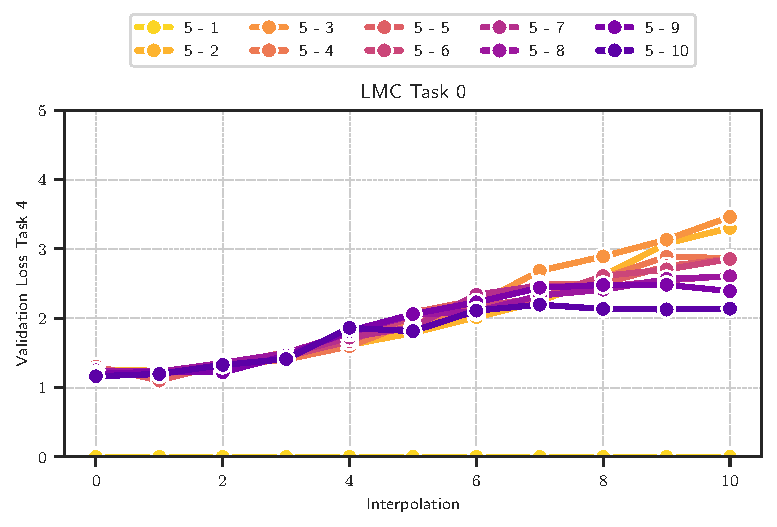
\includegraphics[width=0.3\linewidth]{figures/LMC_task_0_re001.pdf}
    \caption{Comparison of Linear Mode Connectivity between the first task and all subsequent ones with varying dataset fractions. Left: $r=0.5$ (half the dataset). Center: $r=0.1$. Right: $r=0.01$. }
    \label{fig:LMC-Replay-Fraction}
\end{figure}
In \cref{fig:LMC-Replay-Fraction} a clear pattern emerges: using a higher 
fraction of the dataset $r$, the increase in the loss is lower. Moreover, using $r=0.5$ is enough to avoid any increase in the loss. 

\paragraph{Ablation \#2: number of repetitions.}
In this experiment we evaluate LMC while varying the amount of repetitions of the old tasks' data needed to obtain LMC. More specifically, we reduce the number of old tasks which are integrated in the loss from $t$ to a fixed number $o$. The results (shown in \cref{fig:LMC-nrt}) demonstrate that a higher number of task repetitions reduces the increase in loss. Perhaps surprisingly, only 3 tasks repetitions seem sufficient to obtain LMC.  
\begin{figure}[h!]
    \centering
    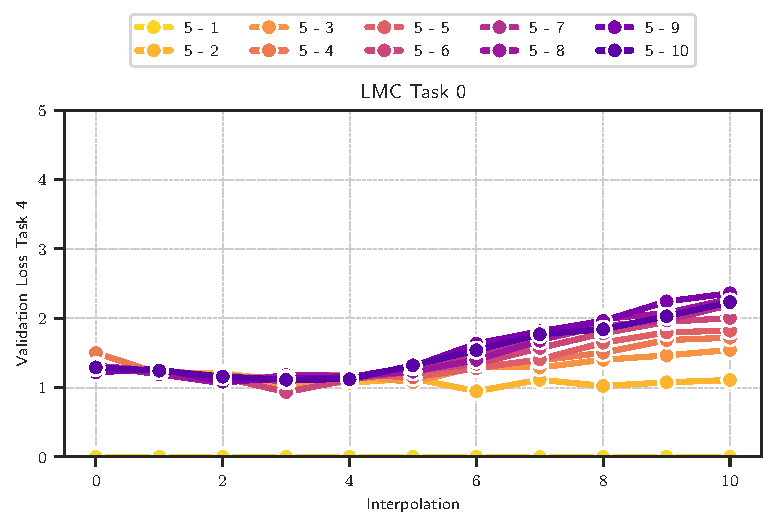
\includegraphics[width=0.3\linewidth]{figures/LMC_task_0_rt1.pdf}
    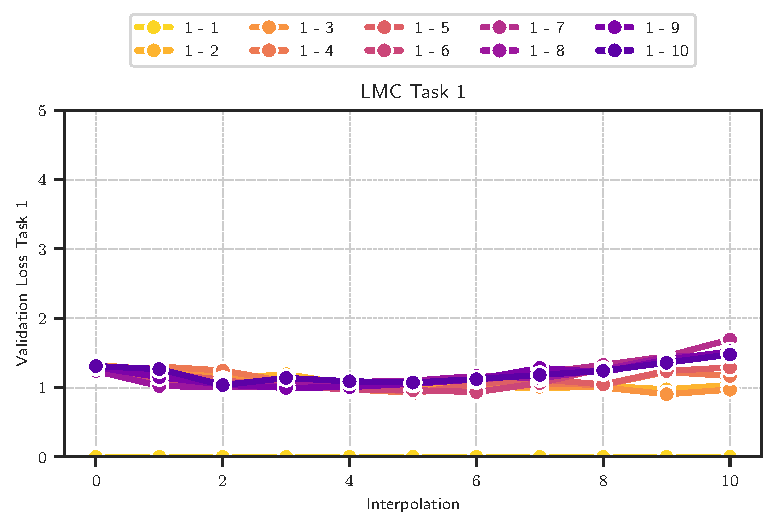
\includegraphics[width=0.3\linewidth]{figures/LMC_task_0_nrt2.pdf}
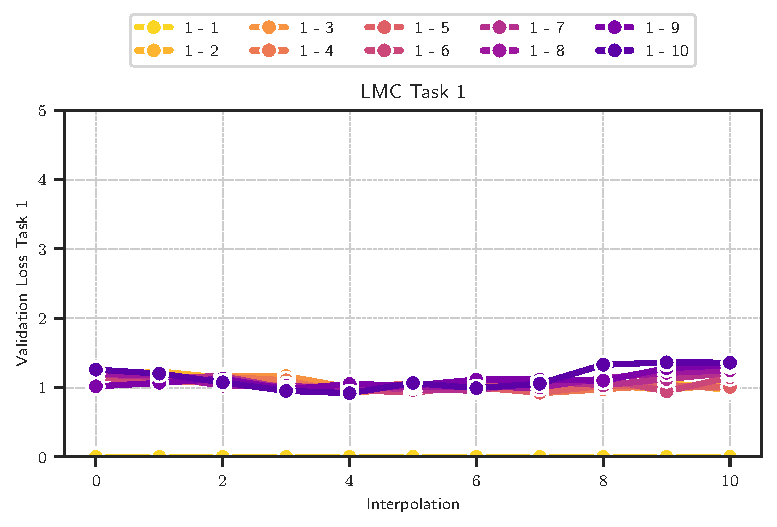
\includegraphics[width=0.3\linewidth]{figures/LMC_task_0_nrt3.pdf}
    \caption{Comparison of Linear Mode Connectivity between the first task and all subsequent ones with varying number of repetitions. Left: $o=1$. Center: $o=2$. Right: $o=3$.  }
    \label{fig:LMC-nrt}
\end{figure}

\newpage

\section{Research questions}
\label{sec:RQ}
\paragraph{Research question \#1.} The local nature of parameter-based approximations relying on regularization makes them inept in scenarios where the task loss geometric structure is very dynamic. The first question is whether the consolidation process observed when incorporating the old task losses in the objective reduces the change in the task loss geometry, thereby extending the validity of the parameter-based approximation. 

\paragraph{Q \#1.1} Does the consolidation process have lasting effects, such that after some $K$ repetitions, the old task loss geometry is guaranteed not to change? If this were the case, then the data-based approximation of the old task loss could effectively be replaced by an equally valid parameter-based approximation. 

\paragraph{Q \#1.2} How much data is needed for the consolidation process to take place? The experiments in  \citet{mirzadeh_linear_2020-1} compute the old tasks loss on the full training dataset. Can the same results be achieved with less data? 

\paragraph{Q \#1.3} How is the consolidation process dependent on the model size and data similarity? 


\paragraph{Research question \#2.} The error of a second order approximation of the task loss is in the order of its third order terms. How does the approximation error change during the consolidation process? 

\paragraph{Q \#2.1} In general, how do data-based and parameter-based approximations relate? 

\paragraph{Q \#2.2} Which data is important for the second-order expansion error? 

\paragraph{Q \#2.3} Does the consolidation process decrease the third order term in the expansion? 


\newpage



\newpage

\section{Old derivations (to throw away)}

\subsection{Linear Mode Connectivity}

\begin{figure}
    \centering
    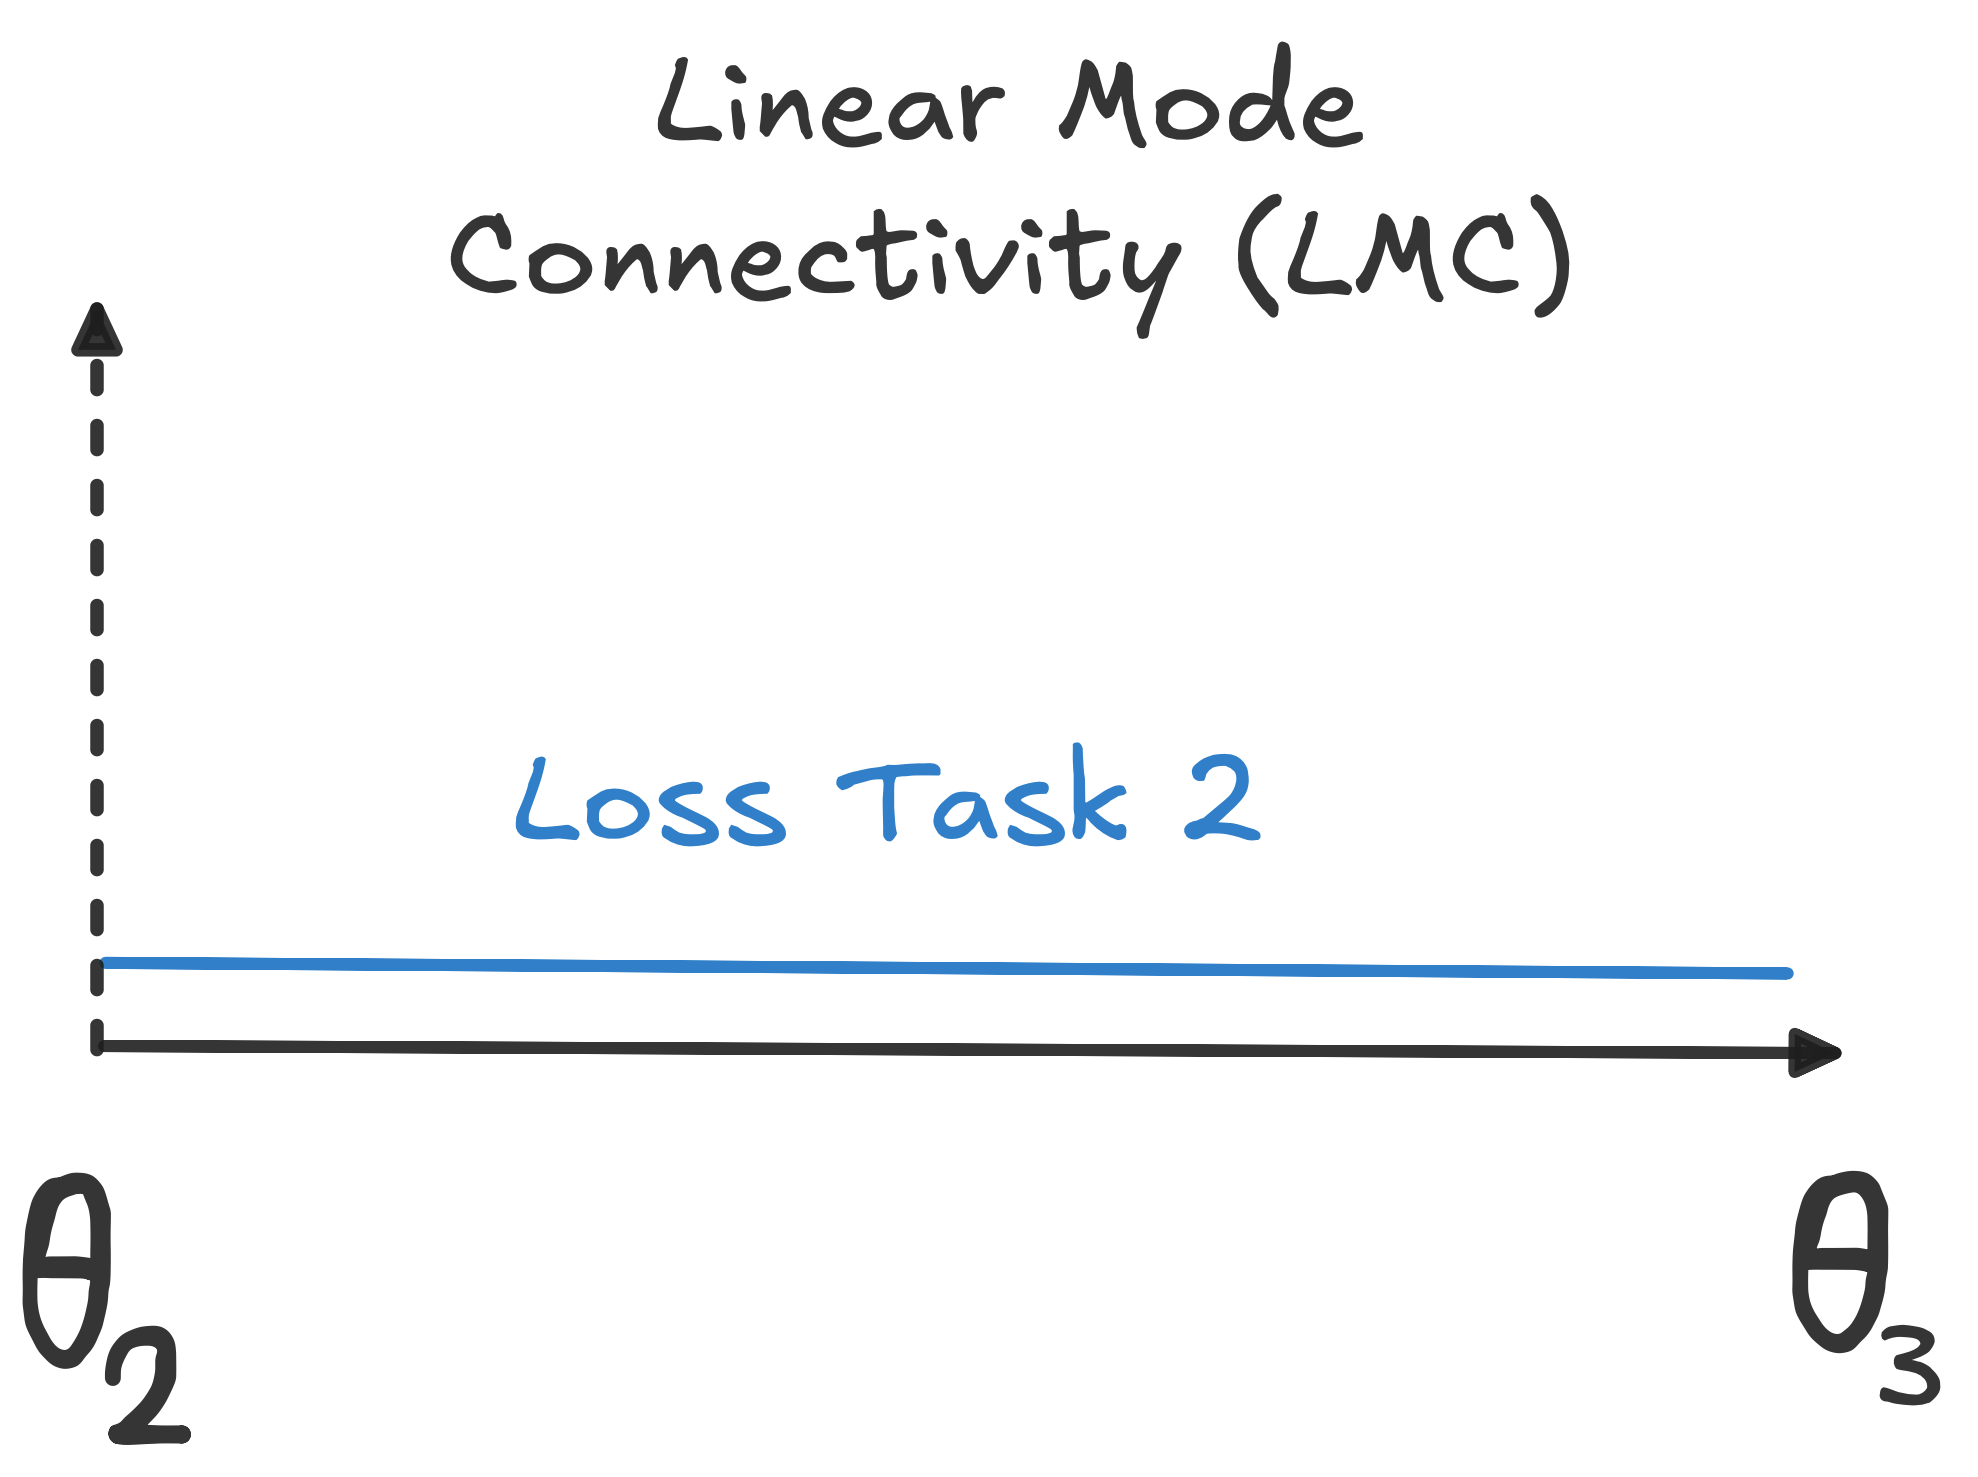
\includegraphics[width=0.28\linewidth]{figures/LMC.png}
    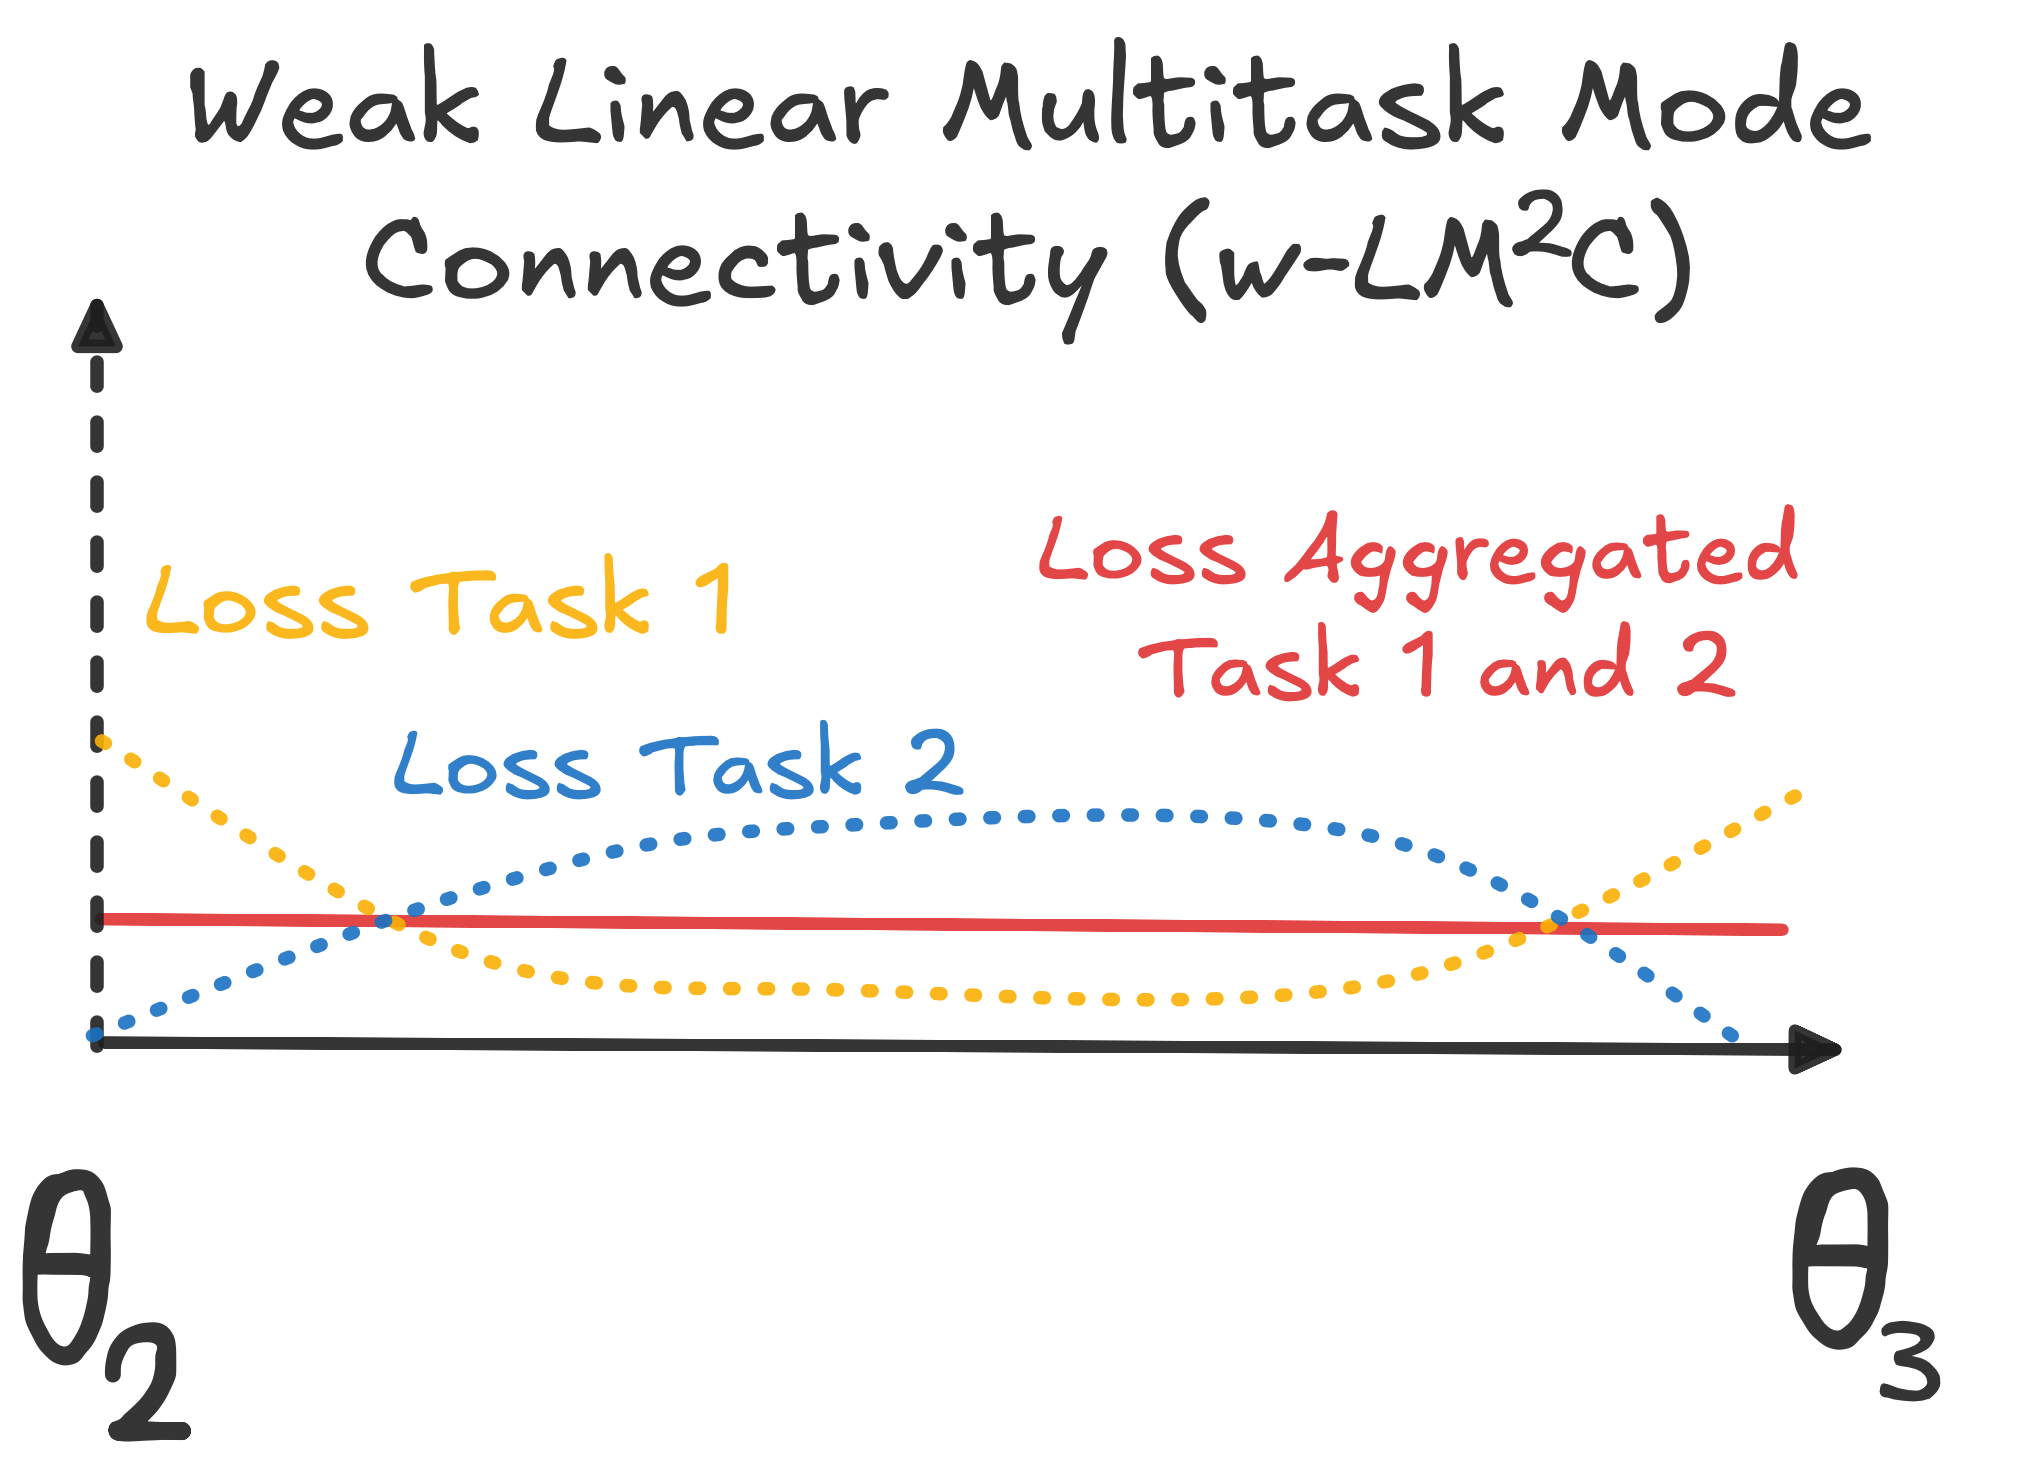
\includegraphics[width=0.3\linewidth]{figures/wLM2C.png}
    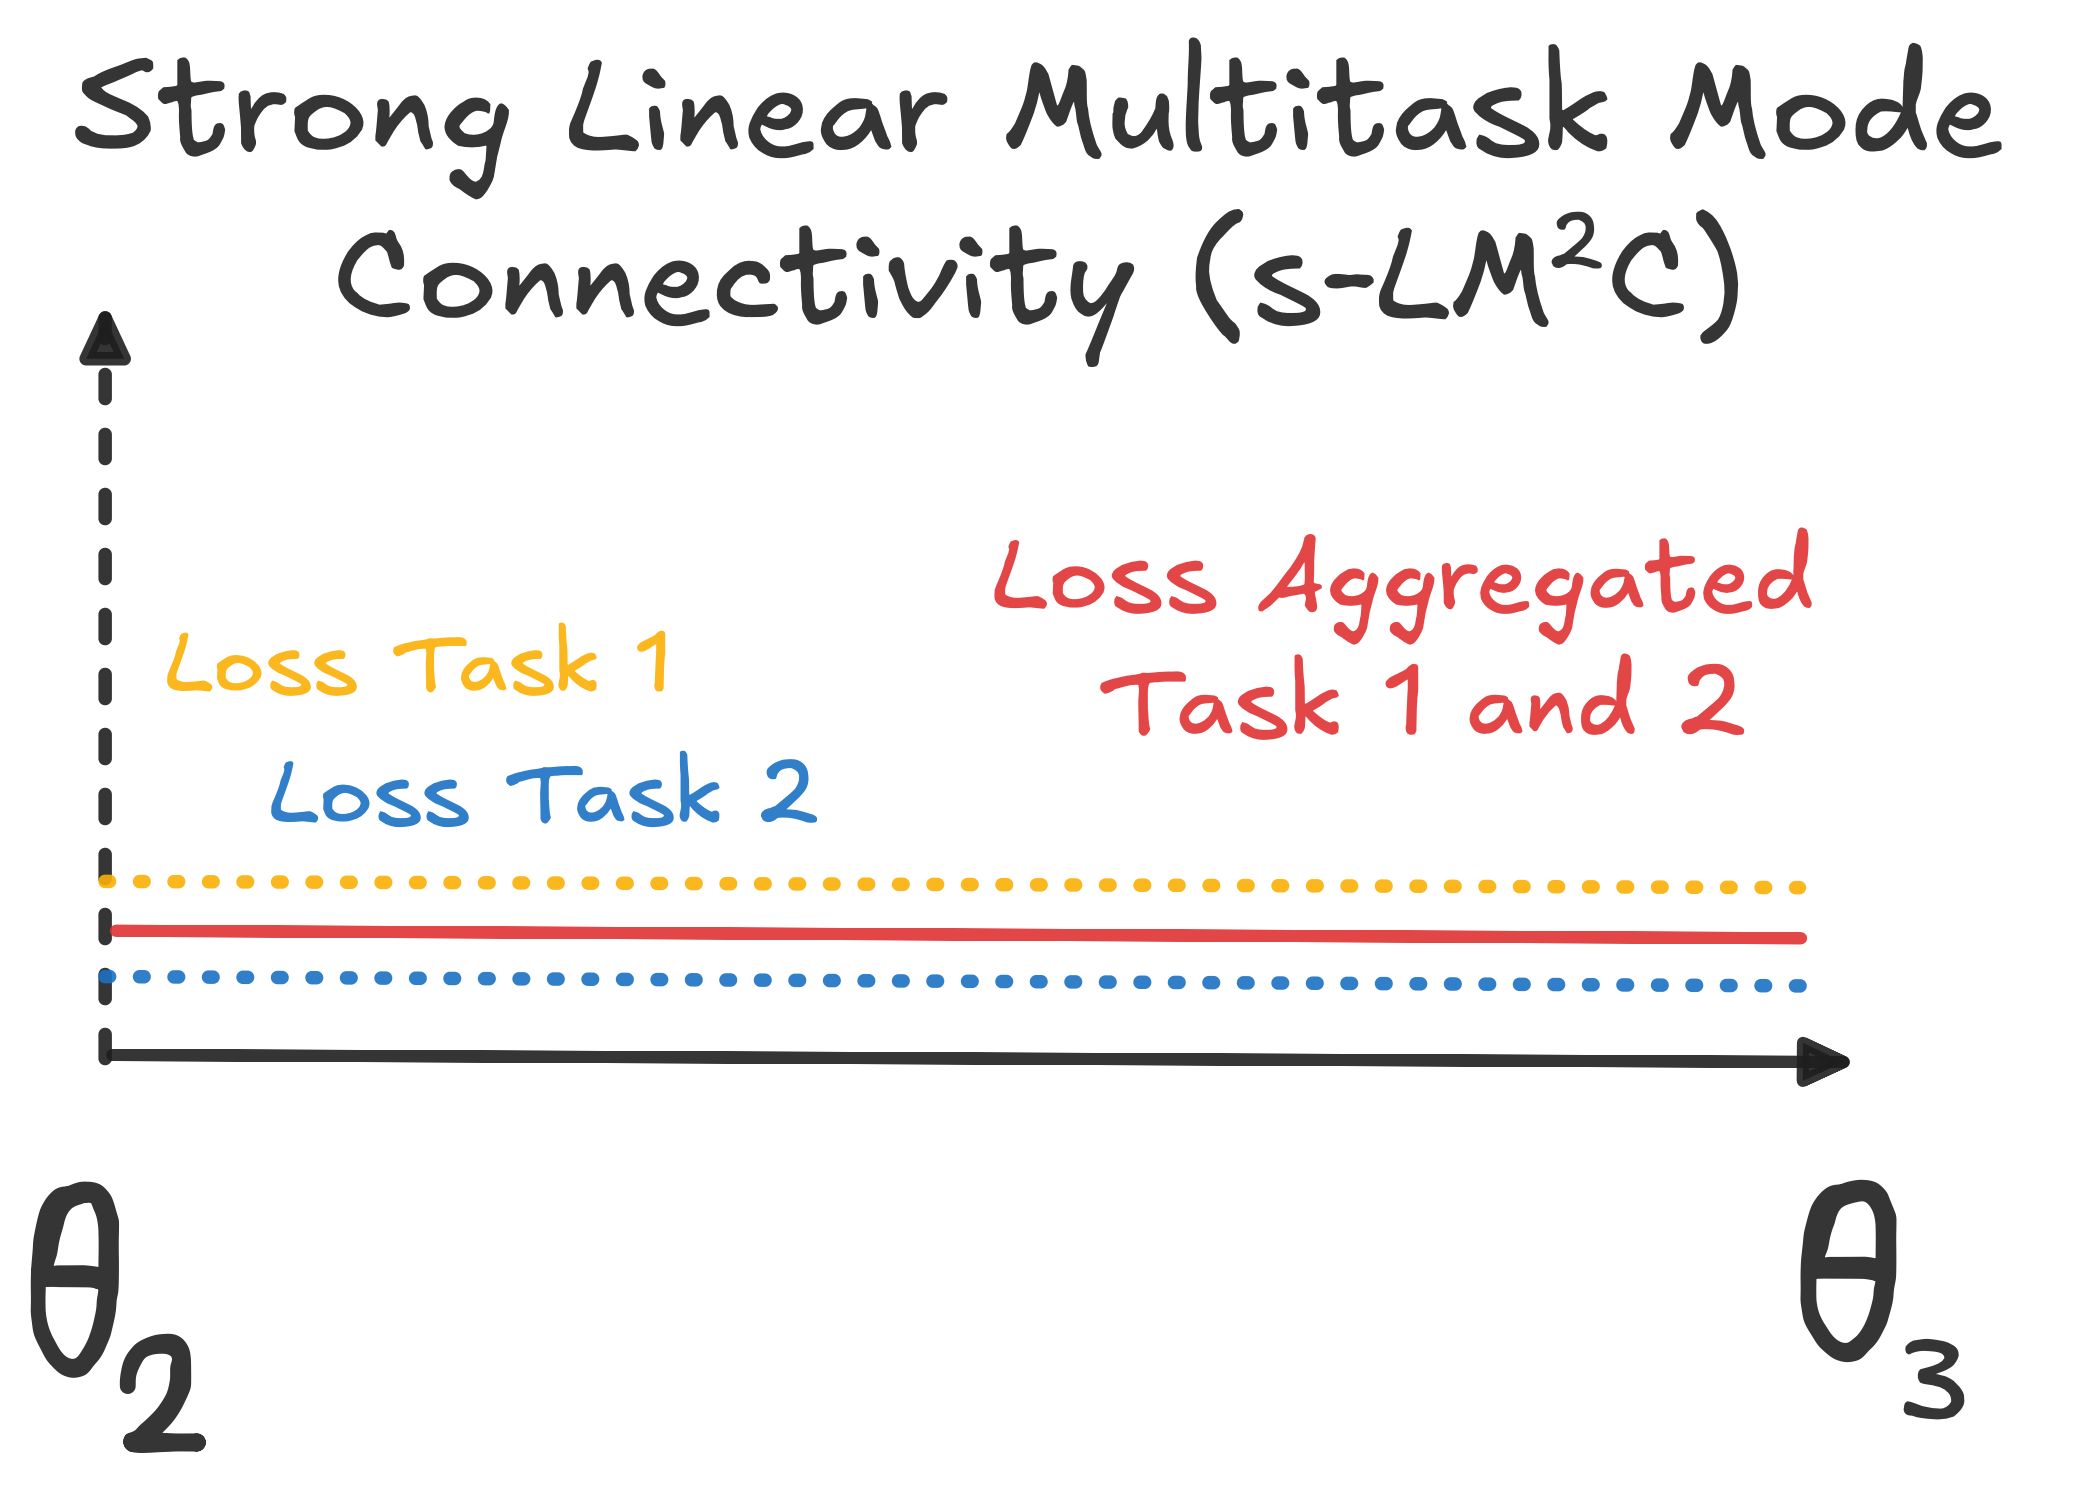
\includegraphics[width=0.3\linewidth]{figures/sLM2C.png}
    \caption{
    Illustrative sketch of LMC (\cref{def:LMC}), w-LM$^2$C (\cref{def:weak-LM2C}) and s-LM$^2$C (\cref{def:strong-LM2C}).
    }
    \label{fig:sketch-definitions}
\end{figure}

% Let $\vDelta_{t_1t_2} = \vparam_{t_2} - \vparam_{t_1}$ be the parameter displacement vector moving from task $t_1$ to task $t_2$. 

% \textcolor{forestgreen}{\textbf{Goal.}} We want to prove that, if there is LMC across all minima, then there must be a common low-curvature subspace shared across all tasks. 

% More formally. 

\begin{defn}[Linear Mode Connectivity (LMC)]
    Let $\vparam_1, \vparam_2$ be two points in the parameter space, and define the linear interpolation function $l_{12}(\kappa) = \kappa\cdot \vparam_{2} + (1-\kappa)\cdot \vparam_{1}$. Given a loss function $\loss(\vparam, \data)$ we say that there is Linear Mode Connectivity from $\vparam_{1}$ to $\vparam_{2}$ if the loss is \emph{constant over the curve $\{l_{12}(\kappa), \kappa \in [0,1]\}$}:
\begin{align}
    \deriv{\loss(l_{12}(\kappa), \data)}{\kappa} = 0 \hspace{1cm}\forall \:\kappa \in [0,1]
\end{align}
\end{defn}

\todo{Generalize the notion of LMC to non-increasing loss.}


\begin{thm}[Preservation of the null-space by learning.]
\label{theo:preservation-of-null space}
\todo{Needs to be rewritten}
If there is LMC  $\vparam_{t_1} \ra \vparam_{t_2}$, where $\vparam_{t_1}$ and $\vparam_{t_2}$ are local minima of the loss $\loss(\vparam, \data_{1:t_1}$ and ... 
then the intersection  of the Hessians $\hessian(\vparam_{1}, \data), \hessian(\vparam_{2}, \data)$ null spaces is not-empty, i.e. (some of) the null-space structure is preserved by learning. Furthermore, the parameter displacement $\vDelta_{12}$ lies in the intersection.
\end{thm}


\begin{proof}
Define the linear interpolation between $\vparam_1, \vparam_2$ as $l_{12}(\kappa) = \kappa\cdot \vparam_2 + (1-\kappa)\cdot \vparam_1$, where $\kappa \in [0,1]$. 
%Our experiments show that the loss $\loss(l_{12}(\kappa), \data_{t_1})$ is \emph{constant over the curve $\{l_{12}(\kappa), \kappa \in [0,1]\}$}. Equivalently we say: 
By LMC (\cref{def:LMC}) we have:
\begin{align}
    &\deriv{\loss(l_{12}(\kappa), \data)}{\kappa} = 0 \hspace{1cm}\forall \:\kappa \in [0,1]\\
    \label{eq:condition-on-grad}
    & \hspace{3pt} = \deriv{\loss(l_{12}(\kappa), \data)}{l_{12}(\kappa)}^\top \deriv{l_{12}(\kappa)}{\kappa} = \grad_{l_{12}(\kappa)}\loss(l_{12}(\kappa), \data) ^\top \vDelta_{12} = 0 \hspace{1cm}\forall \:\kappa \in [0,1]
\end{align}
Consider now the second-order approximation of the loss around $l_{12}(\kappa)$ for a small perturbation $\delta\kappa$\footnote{Note that $\delta\kappa$ can be arbitrarily small, so the result is quite solid.}: 
\begin{align}
    \underbrace{\loss(l_{12}(\kappa + \delta\kappa), \data) - \loss(l_{12}(\kappa), \data)}_{=0 \text{ by LMC}} \approx  
    & \hspace{3pt} \underbrace{(\delta\kappa\,\vDelta_{12})^\top\grad_{(l_{12}(\kappa)}\loss((l_{12}(\kappa), \data)}_{=0 \text{ by \cref{eq:condition-on-grad}}} \\
    & \hspace{3pt}+ (\delta\lambda\,\vDelta_{12})^\top\hessian((l_{12}(\lambda), \data)(\delta\lambda\,\vDelta_{12}),
\end{align}
Therefore we have the second order condition: 
\begin{equation}  
\label{eq:second-order-condition}
\vDelta_{12}^\top\hessian((l_{12}(\lambda), \data)\vDelta_{12} = 0 \hspace{1cm}\forall \:\lambda \in [0,1]
\end{equation}
For $\|\vDelta_{12}\| > 0$ this implies that $\vDelta_{12}$ lies in the \emph{null-space} of the Hessian of task $t_1$, computed at $l_{12}(\lambda)$, for all $\lambda \in [0,1]$. By \cref{prop:intersection-of-nullspaces}, this means that the displacement vector $\vDelta_{12}$ \emph{must lie at the intersection of all such subspaces}. 

\begin{prop}
\label{prop:intersection-of-nullspaces}
Let $\mathcal{N}(\lambda) = \nullspace(\hessian((l_{12}(\lambda), \data))$, and let $\mathcal{N}_{\intersect} = \intersect_{\lambda \in [0,1]} \mathcal{N}(\lambda)$. Then if $\vDelta_{12} \notin \mathcal{N}_{\intersect}$, there exists $\lambda \in [0,1]$ such that \cref{eq:second-order-condition} is violated.
\end{prop}
\begin{proof}
    Let $\hessian(l_{12}(\lambda), \data) = \vV_{\lambda}\vD_{\lambda} \vV_{\lambda}^\top$ be the eigendecomposition of the Hessian computed at $l_{12}(\lambda)$, with eigenvectors $\vv_1, \dots, \vv_P$ and eigenvalues $d_1, \dots, d_P$. Since $\vV$ forms a basis for the parameter space, we can rewrite $\vDelta_{12} = \sum_k  (\vDelta_{12}^\top \vv_k) \cdot \vv_k$. Letting $\vDelta_{12}^\top \vv_k = \sigma_k$ we rewrite \cref{eq:second-order-condition}: 
    \begin{align}
        \vDelta_{12}^\top\hessian((l_{12}(\lambda), \data)\vDelta_{12} 
        & = \rnd{\sum_{k} \sigma_k \cdot \vv_k}^\top \hessian((l_{12}(\lambda), \data)\rnd{\sum_{k} \sigma_k \cdot \vv_k}\\
        & = \rnd{\sum_k \sigma_k d_k \cdot \vv_k}^\top \rnd{\sum_{k} \sigma_k\cdot \vv_k}\\
        & = \sum_k \sigma_k^2 d_k = \sum_{k\in I^+}\sigma_k^2 |d_k| - \sum_{k\in I^-}\sigma_k^2 |d_k|  
    \end{align}
    
    
    $B$ be a basis in the parameter space and $B_{\intersect}$ be a basis for $\mathcal{N}_{\intersect}$. Then $\vDelta_{12}$ can be expressed as the linear combination $\vDelta_{12} = \sum_{k} (\vDelta_{12}^\top \vb_k) \cdot \vb_k$, where $\vb_i$ is the $i^{th}$ element in the basis $B$. The fact that $\vDelta_{12} \notin \mathcal{N}_{\intersect}$ is equivalent to saying that there exist at least one index $j$ such that $\vb_j$ such that $\vb_j^\top \vDelta_{12} \neq 0$ and $\vb_j \notin \mathcal{N}_{\intersect}$. Rewriting \cref{eq:second-order-condition}: 
    \begin{align*}
        \vDelta_{12}^\top\hessian((l_{12}(\lambda), \data)\vDelta_{12} 
        & = \rnd{\sum_{k} (\vDelta_{12}^\top \vb_k) \cdot \vb_k}^\top \hessian((l_{12}(\lambda), \data)\rnd{\sum_{k} (\vDelta_{12}^\top \vb_k) \cdot \vb_k}\\
        & = \sum_{k, k'} \rnd{ (\vDelta_{12}^\top \vb_k) \cdot \vb_k}^\top \hessian((l_{12}(\lambda), \data)\rnd{ (\vDelta_{12}^\top \vb_{k'}) \cdot \vb_{k'}}\\
        & = \underbrace{(\vDelta_{12}^\top \vb_j)^2}_{\neq 0}\, \underbrace{\vb_j^\top \hessian((l_{12}(\lambda), \data)\vb_{j}}_{\neq 0} \\
        & \neq 0
    \end{align*}
\end{proof} 


Therefore it must be that $\vDelta_{12} \in \mathcal{N}_{\intersect}$, and thus $\rank(\mathcal{N}_{\intersect}) > 0$. 

This concludes the proof of \cref{theo:preservation-of-null space}. 
\end{proof}


\begin{defn}[Weak Linear Multitask Mode Connectivity (w-LM$^2$C)]
\label{def:weak-LM2C}
    Let $\vparam_{t_1}, \vparam_{t_2}$ be two minimizers of the respective multitask loss $\loss(\vparam, \data_{1:t_1}), \loss(\vparam, \data_{1:t_2})$, with $t_2>t_1$, and define the linear interpolation function $l_{t_1t_2}(\lambda) = \lambda\cdot \vparam_{t_2} + (1-\lambda)\cdot \vparam_{t_1}$. Then we say that there is Weak Linear Multitask Mode Connectivity from $\vparam_{t_1}$ to $\vparam_{t_2}$ if the multitask loss on $\data_{1:t_1}$ is \emph{constant over the curve $\{l_{t_1t_2}(\lambda), \lambda \in [0,1]\}$}:
\begin{align}
    \deriv{\loss(l_{t_1t_2}(\lambda), \data_{1:t_1})}{\lambda} = 0 \hspace{1cm}\forall \:\lambda \in [0,1]
\end{align}
\end{defn}
\vspace{0.2cm}
\begin{defn}[Strong Linear Multitask Mode Connectivity (s-LM$^2$C)]
\label{def:strong-LM2C}
    Let $\vparam_{t_1}, \vparam_{t_2}$ be two minimizers of the respective multitask loss $\loss(\vparam, \data_{1:t_1}), \loss(\vparam, \data_{1:t_2})$, with $t_2>t_1$, and define the linear interpolation function $l_{t_1t_2}(\lambda) = \lambda\cdot \vparam_{t_2} + (1-\lambda)\cdot \vparam_{t_1}$. Then we say that there is Strong Linear Multitask Mode Connectivity from $\vparam_{t_1}$ to $\vparam_{t_2}$ if for each task $t\in [1,t_1]$ the loss $\data_{t}$ is \emph{constant over the curve $\{l_{t_1t_2}(\lambda), \lambda \in [0,1]\}$}:
\begin{align}
    &\deriv{\loss(l_{t_1t_2}(\lambda), \data_{1})}{\lambda} = \dots = \deriv{\loss(l_{t_1t_2}(\lambda), \data_{t_1})}{\lambda} = 0 \hspace{1cm}\forall \:\lambda \in [0,1]
\end{align}
\end{defn}
\vspace{0.2cm}
\begin{corr}
\label{corr:SLM2C-implications}
    \todo{write} s-LM$^2$C implies w-LM$^2$C and LMC. (but not viceversa)
\end{corr}
\vspace{0.2cm}
\begin{corr}
\label{corr:SLM2C-implications2}
    \todo{write} If $\{\hessian(\vparam_{t_1}, \data_{1}),\dots, \hessian(\vparam_{t_1}, \data_{t_1}),\hessian(\vparam_{t_2}, \data_{1}),\dots,\hessian(\vparam_{t_2}, \data_{t_1})\}$  are all PSD then s-LM$^2$C and w-LM$^2$C are equivalent, and they both imply LMC. 
\end{corr}
\vspace{0.2cm}
\begin{thm}
\label{theo:preservation-of-multitask-nullspace}
    If for $t_1 < t_2$ there is s-LM$^2$C from $\vparam_{t_1}$ to $\vparam_{t_2}$ then the intersection of the Hessians $\{\hessian(\vparam_{t_1}, \data_{1}),\dots, \hessian(\vparam_{t_1}, \data_{t_1}),\hessian(\vparam_{t_2}, \data_{1}),\dots,\hessian(\vparam_{t_2}, \data_{t_1})\}$ null-space is not-empty, and the parameter displacement $\vDelta_{t_1t_2}$ lies in the intersection.
\end{thm}
\begin{proof}
    We derive this result directly from \cref{theo:preservation-of-null space}. 

    Let $\mathcal{N}(\vparam_{i}, \data_{j}) = \nullspace(\hessian(\vparam_{i}, \data_{j}))$.
    By \cref{def:strong-LM2C} we know that on the line $l_{t_1t_2}(\lambda)$ the loss of each task $t\in[1,t_1]$ is constant. Using the proof of \cref{theo:preservation-of-null space}, substituting $\data_{t_1}$ by $\data_t$ for all $t\in[1,t_1]$ we obtain the following set of conditions:
\begin{equation*}
    \begin{cases}
        \vDelta_{t_1t_2} \in \mathcal{N}(\vparam_{t_1}, \data_{1}) \intersect \mathcal{N}(\vparam_{t_2}, \data_{1}) \\
        \vdots \\
        \vDelta_{t_1t_2} \in \mathcal{N}(\vparam_{t_1}, \data_{t_1}) \intersect \mathcal{N}(\vparam_{t_2}, \data_{t_1})
    \end{cases}
\end{equation*}
Thus combining all the conditions it must be that:
\begin{equation}
    \vDelta_{t_1t_2} \in \bigcap_{\substack{t \in [1,t] \\ i \in \{t_1, t_2\}}} \mathcal{N}(\vparam_{i}, \data_{t})
\end{equation}
and since $\|\vDelta_{t_1t_2}\|>0$ then $\rank\rnd{\bigcap_{\substack{t \in [1,t] \\ i \in \{t_1, t_2\}}} \mathcal{N}(\vparam_{i}, \data_{t})} > 0$. 

This concludes the proof of \cref{theo:preservation-of-multitask-nullspace}.
\end{proof}

\subsection{Hessian nullspace analysis}

\lighthline

\paragraph{Thoughts on the result \cref{theo:preservation-of-null space} and \cref{theo:preservation-of-multitask-nullspace}.} 
\begin{enumerate}
    \item \textbf{On the difference between replay and regularization.} \todo{readjust this} \cref{theo:preservation-of-null space,theo:preservation-of-multitask-nullspace} shows that replay has two effects: (1) preserving a common null space structure across tasks, and (2) forcing the parameters updates to lie in this subspace. Second-order regularization methods also achieve (2) by penalizing the displacement in the tasks' range subspaces. In particular, a general formulation of second-order regularizers is: 
    \begin{equation}
    \label{eq:second-order-reg}
        \reg(\vDelta) = \vDelta^\top\rnd{\sum_{i=1}^{t-1}\hessian(\vparam, \data_i)}\vDelta, 
    \end{equation}
    where $t$ is the task current to the algorithm. Two considerations: 
    \begin{enumerate}
        \item In order to avoid re-computing the Hessian matrices after every update, $\hessian(\vparam_i, \data_i)$ is used instead, and computed once for each task. $\hessian(\vparam_i, \data_i)$ is typically assumed to be PSD. 
        \item Let $\mathcal{P}(\data_i), \mathcal{N}(\data_i)$ be, respectively, the range subspace and null space of $\hessian(\vparam_i, \data_i)$, and $\mathcal{P}_{\union} = \union_{i=1}^{t-1} \mathcal{P}(\data_i)$, and similarly $\mathcal{N}_{\intersect} = \intersect_{i=1}^{t-1} \mathcal{N}(\data_i)$. There are two ways to minimize \cref{eq:second-order-reg}: (1) compute $\mathcal{P}_{\union}$ and enforce $\vDelta \notin  \mathcal{P}_{\union}$ or compute $\mathcal{N}_{\intersect}$ and enforce $\vDelta \in \mathcal{N}_{\intersect}$. 
        The first approach is advantageous early in training, as the Hessian of neural networks around loss minima is known to have a low rank structure, and thus computing $\mathcal{P}_{\union}$ is cheap. However, as the number of tasks processed increases, $\dim(\mathcal{P}_{\union})$ increases, while $\dim(\mathcal{N}_{\intersect})$ decreases, and thus computing directly $\mathcal{N}_{\intersect}$ is more advantageous later in training.\footnote{Interestingly, typically continual learning methods take first approach.}\footnote{Based on the observed LMC property, We have reached a unified formulation of replay and regularization.} 
    \end{enumerate}
    Thus, both replay and second-order regularization methods aim to enforce condition (2): $\vDelta \in \mathcal{N}_{\intersect}$. However, for this condition to be meaningful, condition (1) must also hold. Unlike replay, regularization methods do not ensure that the null space (or, equivalently, the range subspace) remains stable during training—an absence that fundamentally limits their effectiveness.
    \item \textbf{On the role of scale and data similarity.} The dimensionality of $\mathcal{N}_{\intersect}$ shrinks as more tasks are introduced. When $\dim(\mathcal{N}_{\intersect})=0$ learning stops. A key question is: how rapidly does this reduction occur? The answer depends on how geometrically similar the tasks are. If two tasks share no overlap in their structures, the model cannot learn both. However, since the null space is typically high-dimensional, such a scenario is rare. On the other end of the spectrum, if all tasks are effectively the same, the null space remains unchanged. This consideration leads to a second factor in $\dim(\mathcal{N}_{\intersect})$: the number of parameters of the model. Scaling the model dimensionality should enable learning a greater number of tasks -- unless the dimensionality of the range subspace also scales with the model. Thus an important open question is how $\mathcal{N}_{\intersect}$ scales with (1) the data, and (2) the model size. 
\end{enumerate}


Now we move on to ask the question: \emph{why does gradient descent with the multitask objective yield s-LM$^2$C?}

By \cref{theo:preservation-of-multitask-nullspace} there are two concurrent conditions which must be satisfied to obtain s-LM$^2$C, namely: the task update $\vDelta_{t,t+1}$ must lie in the intersection of the Hessians $\hessian(\vparam_t, \data_{1:t}),\hessian(\vparam_{t+1}, \data_{1:t})$ null-space; such an intersection must be non-empty. In this section we take on a dynamical systems view of the Hessian spectrum, and study how it evolves during optimization for a general class of losses. 

\vspace{0.5cm}



\lighthline


Recall that the multitask objective of task $t$ is
\begin{equation}
    \loss(\vparam, \data_{1:t}) = \frac{1}{t} \rnd{\loss(\vparam, \data_1) + \dots + \loss(\vparam, \data_t)}
\end{equation}
If $\vparam_t$ is a local minima of the multitask loss of task $t$, then the following conditions hold: 
\begin{align}
    \label{eq:opt-condition2}
    &\nabla_{\vparam_t}\loss(\vparam_t, \data_{1:t}) = 0\\
    \label{eq:opt-condition3}
    &\hessian(\vparam_t, \data_{1:t}) \succeq 0
\end{align}



Consider now the line from $\vparam_{t}$ to $\vparam_{t+1}$: $l_{t,t+1}(\lambda) = \lambda\cdot \vparam_{t+1} + (1-\lambda)\cdot \vparam_{t}$, $\lambda \in [0,1]$. Alternatively, we can identify any point on the line as $l_{t,t+1}(\lambda) = \vparam_t + \lambda\cdot \vDelta_{t,t+1}$, where $\vDelta_{t,t+1} = \vparam_{t+1} - \vparam_t$ is the parameter displacement vector.


\textcolor{forestgreen}{\textbf{Goal.}} We would like to prove that, in virtue of $\vparam_t$ and $\vparam_{t+1}$ being  local minima of, respectively, $\loss(\vparam, \data_{1:t})$ and $\loss(\vparam, \data_{1:t+1})$ the loss $\loss(\vparam, \data_{i})$ should remain constant on this line, for any $i \in [1,t]$. 


\begin{thm}
\label{theo:formula-loss-change}
    Let $\vparam_1,\vparam_2$ be any two point in the parameter space, and $l_{12}(\lambda)$ the line connecting them. Further, divide the line in $N$ parts with points $\lambda = \frac{1}{N}, \frac{2}{N}, \dots, 1$ and write $\vv = \vparam_2 - \vparam_1$. The change in the loss $\loss(\vparam, \data_1)$ from $\vparam_1$ to $\vparam_2$ is: 
    \begin{equation}
        \loss(\vparam_{2}, \data_{i}) - \loss(\vparam_1, \data_{i}) = \vv^\top\vg_0 + \vv^\top \rnd{ \sum_{r=1}^{N-1} \rnd{ \sum_{r'=0}^{r-1} \hessian_{r'}} + \frac{1}{2}\hessian_r} \vv,
    \end{equation}
    where $\hessian_r = \hessian(l_{12}(\frac{r}{N}), \data_i)$ is the Hessian of the $r$ point on the line and $\vg_0 = \grad_{\vparam_1}\loss(\vparam_1, \data_{i})$.
\end{thm}

\proof{
For any $i \in [1,t]$ we can write the change of the loss on task $i$ along the line path as a sum of the changes on every point of the path. 

\begin{align}
\label{eq:Taylor-linepath}
    \loss(l_{t,t+1}(\lambda + \delta\lambda), \data_{i}) - \loss(l_{t,t+1}(\lambda), \data_{i}) \approx  
    & \hspace{3pt} (\delta\lambda\,\vDelta_{t,t+1})^\top\grad_{l_{t,t+1}(\lambda)}\loss(l_{t,t+1}(\lambda), \data_{i}) \\
    & \hspace{3pt}+ \frac{1}{2}(\delta\lambda\,\vDelta_{t,t+1})^\top\hessian(l_{t,t+1}(\lambda), \data_{i})(\delta\lambda\,\vDelta_{t,t+1}),
\end{align}

Summing over any discretization of $[0,1]$, i.e. $\lambda \in \{\frac{r}{N}\}_{r=1}^{N-1}$ and $\delta\lambda = 1/N$ we get: 
\begin{align}
    \loss(\vparam_{t+1}, \data_{i}) - \loss(\vparam_t, \data_{i}) \approx  \sum_{r = 0}^{N-1} (\delta\lambda)\,\vDelta_{t,t+1}^\top\vg_r + \frac{1}{2}(\delta\lambda)^2\,\vDelta_{t,t+1}^\top\hessian_r\vDelta_{t,t+1},
\end{align}
where for brevity we used $\vg_r=\grad_{l_{t,t+1}(\frac{r}{N})}\loss(l_{t,t+1}(\frac{r}{N}), \data_{i})$ and $\hessian_r = \hessian(l_{t,t+1}(\frac{r}{N}), \data_{i})$

By imposing $\loss(\vparam_{t+1}, \data_{i}) - \loss(\vparam_t, \data_{i}) = 0$ we get the condition
\begin{align}
\label{eq:linepath-condition}
    \sum_{r=0}^{N-1} (\delta\lambda)\,\vDelta_{t,t+1}^\top\vg_r + \frac{1}{2}(\delta\lambda)^2\,\vDelta_{t,t+1}^\top\hessian_r\vDelta_{t,t+1} = 0
\end{align}

Taking the gradient of Taylor expansion in \cref{eq:Taylor-linepath}:
\begin{align}
\label{eq:Taylor-linepath-gradient}
    \grad_{l_{t,t+1}(\lambda + \delta\lambda)}\loss(l_{t,t+1}(\lambda + \delta\lambda), \data_{i}) =
    & \hspace{3pt} \grad_{l_{t,t+1}(\lambda)}\loss(l_{t,t+1}(\lambda), \data_{i}) + \hessian(l_{t,t+1}(\lambda), \data_{i})(\delta\lambda\,\vDelta_{t,t+1})
\end{align}
We rewrite \cref{eq:Taylor-linepath-gradient} as:
\begin{align}
    \vg_n 
    &=  \vg_{n-1} + (\delta\lambda)\,\hessian_{n-1}\vDelta_{t,t+1} = \vg_0 + \sum_{r=0}^{n-1} (\delta\lambda)\hessian_r\vDelta_{t,t+1},
\end{align}
Plugging this result in \cref{eq:linepath-condition} and using \cref{eq:opt-condition2}, i.e. $\vg_0=0$:
\begin{align}
    \sum_{r=1}^{N-1} \rnd{(\delta\lambda)^2 \sum_{r'=0}^{r-1} \vDelta_{t,t+1}^\top\hessian_r\vDelta_{t,t+1}} + \frac{1}{2}(\delta\lambda)^2\,\vDelta_{t,t+1}^\top\hessian_r\vDelta_{t,t+1} = 0
\end{align}
Removing $(\delta\lambda)^2>0$ and factorizing $\vDelta_{t,t+1}$:
\begin{align}
    \vDelta_{t,t+1}^\top \rnd{ \sum_{r=1}^{N-1} \rnd{ \sum_{r'=0}^{r-1} \hessian_{r'}} + \frac{1}{2}\hessian_r} \vDelta_{t,t+1} = 0
\end{align}
}

This result tells us that the behaviour of the loss along this linear path ultimately depends on the inter-relationship of the Hessians computed along the path. If the Hessians are all PSD then it the condition is only verified if they share some parts of the null-space and $\vDelta_{t,t+1}$ resides therein.

This is clearly not the case for any two minimizers of a loss function. The additional structure may come from the sequential nature of the optimization process. 



\paragraph{HESSIAN NULLSPACE STABILITY ANALYSIS}
We here directly ask whether multitask optimization preserves the nullspace of the previous tasks' Hessian. We start with the assumption that $\vparam_t$ is a local minimum for all previous tasks' losses, i.e. \cref{eq:opt-condition2,eq:opt-condition3} apply. 

In particular, let $\vparam(s)$, with $s=1,\dots,L$ denote the steps taken in the iterative optimization process from $\vparam_{t}$ to $\vparam_{t+1}$ ($\vparam(L) = \vparam_{t+1}$).

\textcolor{forestgreen}{We want to show that:}
\begin{equation}
    \vv^\top \hessian(\vparam(s), \data_i) \vv = 0 \,\,\ra \,\,\vv^\top \hessian(\vparam(s+1), \data_i) \vv = 0,
\end{equation}
where by gradient descent we have $\vparam(s) = \vparam(s+1) + \eta\grad{\loss({\vparam(s), \data_{1:t+1}})}$. For convenience we hereafter denote $\grad{\loss({\vparam(s), \data_{1:t+1}})}  = \vg(s)$. Thus $\vparam(s) - \vparam(s+1) = \eta\vg(s)$.

In order to proceed we need to introduce a tool, which is useful to describe the dynamics of the neural network function $\vF(\vparam)$ in a compact way. 

\begin{defn}[Neural Tangent Kernel (NTK)] 
Let $\vF(\vparam, \vx)$ be the output of a neural network with parameters $\vparam$ evaluated at input $\vx \in \real^d$, and assume the output is $O$-dimensional. The Neural Tangent Kernel (NTK) between two inputs $\vx, \vx' \in \real^d$ is defined as: 
\begin{equation} 
\label{eq:ntk-def} 
\vparam_{\vparam}(\vx, \vx') = \grad_{\vparam} \vF(\vparam, \vx)^\top \grad_{\vparam} \vF(\vparam, \vx') \in \real^{O \times O}, \end{equation} 
where the gradients are taken with respect to the parameters $\vparam$. 
\end{defn}


\begin{defn}[Cross-Tasks NTK]  
Let $\data_i = \{\vx^{(i)}_n\}_{n=1}^{N_i}$ and $\data_j = \{\vx^{(j)}_m\}_{m=1}^{N_j}$ be two datasets corresponding to tasks $i$ and $j$, respectively. The \textit{Cross-Tasks Neural Tangent Kernel (NTK)} between $\data_i$ and $\data_j$ is defined as the block matrix:
\begin{equation}
    \label{eq:cross-task-ntk}
    \vparam_{\vparam}(\data_i, \data_j) = 
    \begin{bmatrix}
        \vparam_{\vparam}(\vx^{(i)}_1, \vx^{(j)}_1) & \cdots & \vparam_{\vparam}(\vx^{(i)}_1, \vx^{(j)}_{N_j}) \\
        \vdots & \ddots & \vdots \\
        \vparam_{\vparam}(\vx^{(i)}_{N_i}, \vx^{(j)}_1) & \cdots & \vparam_{\vparam}(\vx^{(i)}_{N_i}, \vx^{(j)}_{N_j})
    \end{bmatrix}
    \in \real^{N_i O \times N_j O},
\end{equation}
where each block entry $\vparam_{\vparam}(\vx^{(i)}_n, \vx^{(j)}_m)$ is given by the NTK between two inputs as in \cref{eq:ntk-def}.
\end{defn}

With \cref{eq:cross-task-ntk} we can express the evolution of the network function on any input $\vx$ as follows.  By gradient descent and linearizing we have:
\begin{align}
    \vF(\vparam(s+1), \vx_n) 
    &=  \vF(\vparam(s), \vx_n) - \eta \grad\vF(\vparam(s), \vx_n) \vg(s)\\
    \label{eq:deriv-step}
    &= \vF(\vparam(s), \vx_n) - \eta \grad\vF(\vparam(s), \vx_n) \rnd{\frac{1}{t+1}\sum_{i=1}^{t+1}{\grad\loss(\vparam(s), \data_i)}}\\
    &= \vF(\vparam(s), \vx_n) - \frac{\eta}{t+1} \grad\vF(\vparam(s), \vx_n) \rnd{\sum_{i=1}^{t+1}\sum_{n'=1}^{N_{i}}\grad\vF(\vparam(s), \vx_{n'})^\top\grad_{\vF}\loss(\vparam(s), \vx_{n'})}
\end{align}
To write everything in a compact way we denote by $\vF(\vparam(s+1), \data_i)$ the $N_i \times O$ dimensional matrix, where each row corresponds to a different sample: 
\begin{equation}
\label{eq:evolution-net-output}
    \vF(\vparam(s+1), \data_i) = \vF(\vparam(s), \data_i) - \frac{\eta}{t+1}\sum_{j=1}^{t+1}\vparam_{\vparam}(\data_i, \data_{j})\grad_{\vF}\loss(\vparam(s), \data_{j})
\end{equation}
From \cref{eq:evolution-net-output} it is clear to see that the cross-tasks NTK plays a central role in the evolution of the network function on the dataset $\data_i$. 


We can express $\hessian(\vparam(s+1), \data_i)$ as a function of $\hessian(\vparam(s), \data_i)$ using a simple Taylor expansion around $\vparam(s)$:
\begin{equation}
    \label{eq:hessian-correction}
    \hessian(\vparam(s+1), \data_i) = \hessian(\vparam(s), \data_i) - \eta \grad_{\vparam}{\hessian(\vparam(s), \data_{i})} \, \vg(s)
    %\sum_k  \dfrac{\partial \hessian(\vparam(s), \data_{i})}{\partial \param(s)_k}\, g(s)_k
\end{equation}
where $ \grad_{\vparam}{\hessian(\vparam(s), \data_{i})}$ is a three-dimensional tensor (one matrix per network parameter). 

Consider the following decomposition of the Hessian, based on the compositionality of the loss function $\loss(\vparam, \vx) = c\circ\vF(\vparam,(\vx, y))$, where $c$ is a convex cost function (typically a log-likelihood) and $\vF(\vparam,\vx)$ is the function implemented by the network: 
\begin{align}
    \label{eq:Hessian-decomposition}
    \hessian(\vparam(s), \data_{i}) 
    = \frac{1}{N_i} \sum_{n=1}^{N_i} & \grad{\vF(\vparam(s),\vx_n) \left[\frac{\partial^2\loss(\vparam(s), (\vx_n, y_n))}{\partial\vF(\vparam(s), \vx_n)^2}\right]\grad\vF(\vparam(s),\vx_n)^\top } \\
    & + \sum_{k=1}^O \frac{\partial \loss(\vparam(s), (\vx_n, y_n))}{\partial \vF(\vparam(s), \vx_n)_k} \cdot \grad^2\vF(\vparam(s), \vx_n)_k
\end{align}
For the MSE cost function, the loss Hessian with respect to the network output is the identity, so simply: 
\begin{align}
    \label{eq:Hessian-decomposition-2}
    \hessian(\vparam(s), \data_{i}) 
    = \frac{1}{N_i} \sum_{n=1}^{N_i} &\grad{\vF(\vparam(s), \vx_n)\grad\vF(\vparam(s), \vx_n)^\top } + \sum_{k=1}^O \frac{\partial \loss(\vparam(s), (\vx_n, y_n))}{\partial \vF(\vparam(s), \vx_n)_k} \cdot \grad^2\vF(\vparam(s), \vx_n)_k
\end{align}
If $\vparam(s)$ is a minimizer of the loss on $\data_i$, the second term in the decomposition vanishes as the derivative of the loss is close to $0$. Since our starting point is $\vparam_t$, which is, by assumptions, a local minimum of all previous tasks' losses, \emph{we begin by assuming in an inductive fashion that $\vparam(s)$ is also a local minimum of all previous tasks' losses} and we hope to prove that $\vparam(s+1)$ is too\todo{formalize induction}.  

The first term in this Hessian matrix decomposition is also known as Gauss-Newton matrix:
\begin{align}
    \label{eq:GNM}
    \vG(\vparam(s), \data_{i}) 
    = \frac{1}{N_i} \sum_{n=1}^{N_i} &\grad{\vF(\vparam(s), \vx_n)\grad\vF(\vparam(s), \vx_n)^\top } 
\end{align}


% And thus 
% \begin{align}
%     \loss(\vparam(s+1), \data_{i}) 
%     &= \loss(\vparam(s), \data_{i}) + \frac{\partial \loss(\vparam(s), \data_i)}{\partial \vF(\vparam(s), \data_i)}^\top\rnd{\vF(\vparam(s+1), \data_i)- \vF(\vparam(s), \data_i)}\\
%     &=\loss(\vparam(s), \data_{i}) -\frac{\eta}{t+1} \frac{\partial \loss(\vparam(s), \data_i)}{\partial \vF(\vparam(s), \data_i)}^\top\grad\vF(\vparam(s), \data_i) \rnd{\grad\vF(\vparam(s), \data_{t+1})^\top\grad_{\vF}\loss(\vparam(s), \data_{t+1})}
% \end{align}
% \begin{align}
%     \loss(\vparam(s+1), \data_{i}) 
%     &= \loss(\vparam(s), \data_{i}) - \eta \vg(s)^\top\grad\loss(\vparam(s), \data_{i})\\
%     &= \loss(\vparam(s), \data_{i}) - \eta \rnd{\frac{1}{t+1}\sum_{j=1}^t \underbrace{\grad\loss(\vparam(s), \data_j)}_{\approx \, 0} + \grad\loss(\vparam(s), \data_{t+1})}^\top\grad\loss(\vparam(s), \data_{i})\\
%     &= \loss(\vparam(s), \data_{i}) - \frac{\eta}{t+1} \grad\loss(\vparam(s), \data_{t+1})^\top\grad\loss(\vparam(s), \data_{i})
% \end{align}
% Thus the loss does not increase if the gradients of the new task are not negatively aligned with those of the old task.  

Going back to our derivation, from \cref{eq:GNM}, the Hessian gradient under our assumptions is then\footnote{For gradients of multivariate functions we follow the notation input x output.}:
% \todo{Functional hessian}
% \begin{align}
%     &\grad_{\vparam}{\hessian(\vparam(s), \data_{i})} 
%     = \grad_{\vparam}\rnd{\grad{\vF(\vparam(s)) \left[\frac{\partial^2\loss(\vparam(s), \data_i)}{\partial\vF(\vparam(s))\partial\vF(\vparam(s))}\right]\grad\vF(\vparam(s))^\top } + \sum_{k=1}^O \frac{\partial \loss(\vparam(s), \data_i)}{\partial \vF(\vparam(s), \data_i)_k} \cdot \grad^2\vF(\vparam(s), \data_i)}\\
%     & \;\;\;= \grad^2{\vF(\vparam(s)) \left[\frac{\partial^2\loss(\vparam(s), \data_i)}{\partial\vF(\vparam(s))\partial\vF(\vparam(s))}\right]\grad\vF(\vparam(s))^\top } +   \grad{\vF(\vparam(s))\left[\frac{\partial^2\loss(\vparam(s), \data_i)}{\partial\vF(\vparam(s))\partial\vF(\vparam(s))}\right] \grad^2\vF(\vparam(s))^\top }
% \end{align}
% \todo{formalise} For MSE and the like the loss Hessian with respect to the network output is the identity and we get: 
\begin{align}
    \grad\vG(\vparam(s), \data_{i})
    = \frac{1}{N_i} \sum_{n=1}^{N_i} \underbrace{\grad^2\vF(\vparam(s), \vx_n)}_\text{P x P x O}\underbrace{\grad\vF(\vparam(s), \vx_n)^\top}_\text{O x P} +  \underbrace{\grad\vF(\vparam(s), \vx_n)}_\text{P x O} \underbrace{\grad^2\vF(\vparam(s), \vx_n)^\top}_\text{O x P x P}
\end{align}
Now see that due to the Positive Semi Definite Nature of our Gauss-Newton approximation:
\begin{align}
    \text{if } 
    &\vv^\top \hessian(\vparam(s), \data_{i}) \vv = 0 \\
    & \ra \;\vv^\top \rnd{\sum_{n}\grad{\vF(\vparam(s), \vx_n)\grad\vF(\vparam(s), \vx_n)^\top }}\vv = 0 \\
    & \ra \; \sum_{n}\rnd{\grad\vF(\vparam(s), \vx_n)^\top\vv}^2 = 0 \\
    & \ra \;\vv^\top \grad\vF(\vparam(s), \vx_n) = 0
\end{align}
Thus:
\begin{align}
    \vv^\top \hessian(\vparam(s+1), \data_i)\vv 
    & = \underbrace{\vv^\top\hessian(\vparam(s), \data_i)\vv}_{= \, 0} \\
    & \hspace{1cm}- \frac{\eta}{N_i} \sum_n \vv^\top \grad^2\vF(\vparam(s), \vx_n)\grad\vF(\vparam(s), \vx_n)^\top\vg(s)\vv \\
    & \hspace{1cm}- \frac{\eta}{N_i}\sum_n \underbrace{\vv^\top\grad\vF(\vparam(s), \vx_n)}_{= \, 0} \grad^2\vF(\vparam(s), \vx_n)^\top\vg(s)\vv \\
    &= - \frac{\eta}{N_i} \sum_n \vv^\top\grad^2\vF(\vparam(s), \vx_n)\rnd{\grad\vF(\vparam(s), \vx_n)^\top\vg(s)}\,\vv
    % &= - \eta \vv^\top\grad^2\vF(\vparam(s))\rnd{\grad\vF(\vparam(s))^\top \rnd{\grad\vF(\vparam(s)) \cdot \sum_j\frac{\partial\loss(\vparam(s), \data_j)}{\partial\vF(\vparam(s))}}}\,\vv
    %\sum_k  \dfrac{\partial \hessian(\vparam(s), \data_{i})}{\partial \param(s)_k}\, g(s)_k
\end{align}
By recognizing that 
\begin{equation*}
    -\eta\grad\vF(\vparam(s), \vx_n)^\top\vg(s) = - \frac{\eta}{t+1}\sum_{j=1}^{t+1}\vparam_{\vparam}(\vx_n, \data_{j})\grad_{\vF}\loss(\vparam(s), \data_{j}) 
\end{equation*}
Define 
\[\xi(s, \vv) = \vv^\top \rnd{\hessian(\vparam(s+1), \data_i) - \hessian(\vparam(s), \data_i)}\vv\]
Then we get to the following two equivalent formulations (for small $\eta$). 
\begin{align}
    &\xi(s, \vv) = - \frac{1}{t+1}\,\vv^\top\rnd{  \sum_{j=1}^{t+1} \underbrace{\grad^2\vF(\vparam(s),\data_i)}_\text{P x P x NO} \, \vparam_{\vparam}(\data_i, \data_{j})\grad_{\vF}\loss(\vparam(s), \data_{j})\,}\vv\\
    &\nonumber\\
    &\xi(s, \vv) = \frac{1}{N_i}\sum_{k=1}^O \sum_n\rnd{\vv^\top\grad^2\vF(\vparam(s),\vx_n)_k\,\vv}\cdot\rnd{\vF(\vparam(s+1), \vx_{n})_k-\vF(\vparam(s), \vx_n)_k}
\end{align}
Therefore this analysis brings us to two possibilities, for any pair $(k,n)$: 
\begin{enumerate}
    \item Either $\vv^\top\grad^2\vF(\vparam(s),\vx_n)_{k}\,\vv = 0$; 
    \item Or $\vF(\vparam(s+1)_{k}, \vx_{n}) = \vF(\vparam(s), \vx_{n})_{k}$.
\end{enumerate}
The second possibility would trivially also maintain the loss constant along the optimization path, thus proving the induction step.\todo{Check whether the induction step can be proven also without this.}  However, for the second possibility to be true the following "orthogonality" condition must be verified:
\begin{equation}
\label{eq:ortho-condition}
     \vparam_{\vparam}(\data_i, \data_{j})\grad_{\vF}\loss(\vparam(s), \data_{j}) = 0
\end{equation}
In other words the cross tasks kernel should be orthogonal to the functional gradients of the new task. 
\begin{figure}
    \centering
    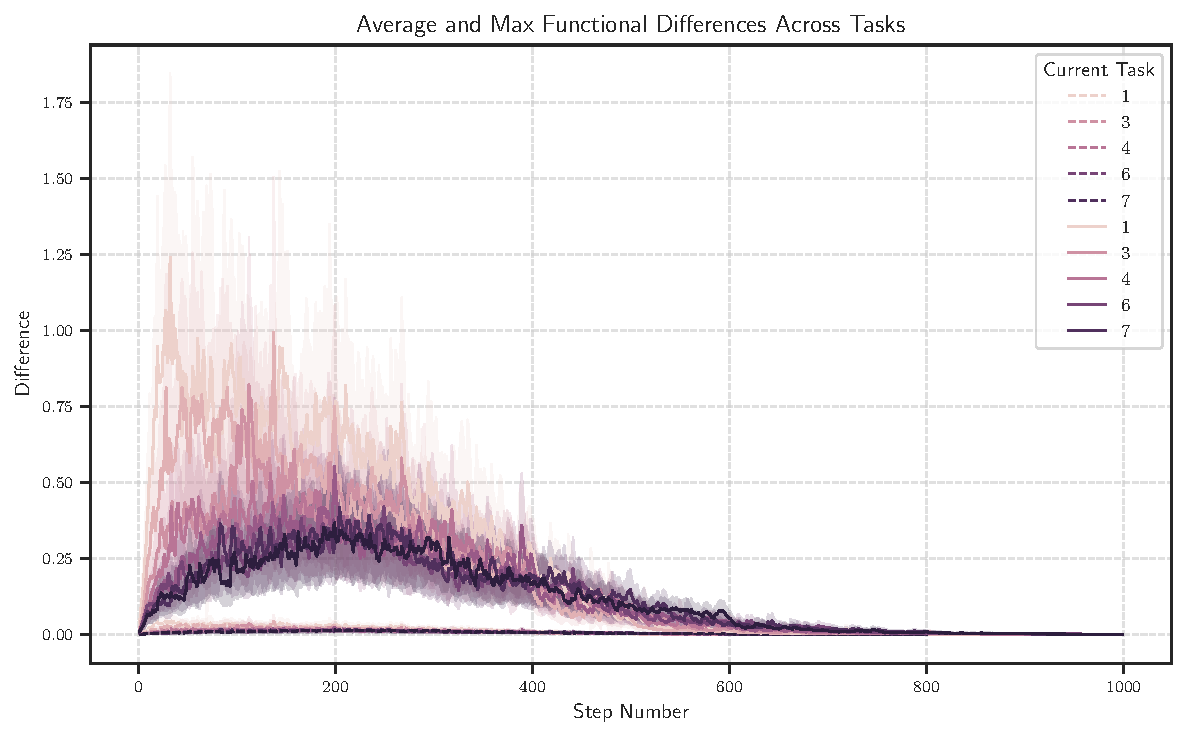
\includegraphics[width=0.7\linewidth]{figures/functional_differences_all_tasks_olddata.pdf}
    \caption{Average (dashed) and Max (full) difference in network function $|\vF(\vparam(s+1),x) - \vF(\vparam(s),x)|$ over the optimization steps $s$. }
    \label{fig:func_diff}
\end{figure}

\begin{figure}
    \centering
    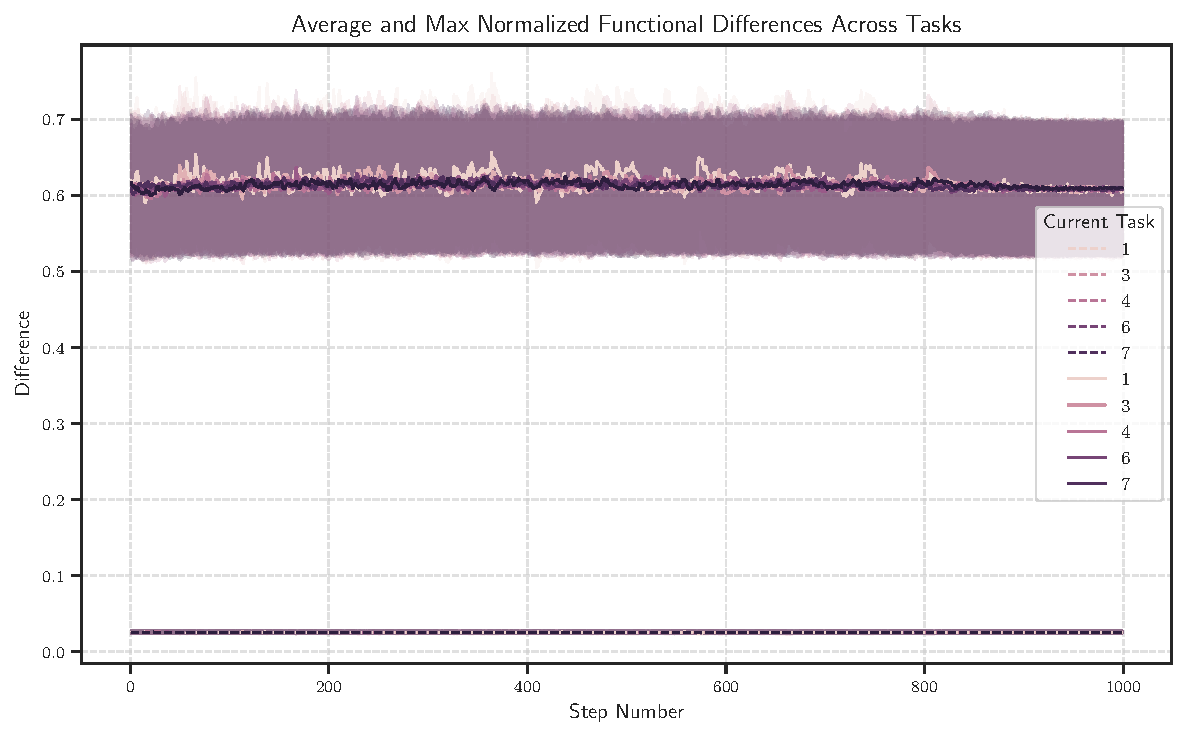
\includegraphics[width=0.7\linewidth]{figures/functional_differences_all_tasks_olddata_normalised.pdf}
    \caption{Normalised average (dashed) and Max (full) difference in network function $|\vF(\vparam(s+1),x) - \vF(\vparam(s),x)|$ over the optimization steps $s$. The normalization factor is the function output norm.}
    \label{fig:func_diff_norm}
\end{figure}

\paragraph{CASE OF TWO TASKS} Consider the simpler case of two tasks, $\data_1, \data_2$. Starting from the same initialization $\vparam_1$, minimizing the multitask and singletask loss will lead to two different endpoints $\vparam_2$. In particular the two optimization processes are characterized by the following distinct dynamics: 
\begin{align}
    &\vparam_{st}(s+1) = \vparam_{st}(s) - \eta\grad\loss(\vparam(s), \data_2) &\text{(Single Task)}\\
    &\vparam_{mt}(s+1) = \vparam_{mt}(s) - \frac{\eta}{2}\rnd{\grad\loss(\vparam(s), \data_2)+\grad\loss(\vparam(s), \data_1)} &\text{(Multi Task)}
\end{align}
Using the above analysis the change in the Hessian of task 1 during optimization is: 
\begin{align}
    \hessian(\vparam(s+1), \data_1) - \hessian(\vparam(s), \data_1) 
    &= - \eta \grad_{\vparam}{\hessian(\vparam(s), \data_1)} \, \vg(s)\\
    &= - \frac{\eta}{N_1} \sum_n \grad^2\vF(\vparam(s), \vx_n)\rnd{\grad\vF(\vparam(s), \vx_n)^\top\vg(s)} \\
    &= - \frac{\eta}{N_1} \sum_n \sum_k \grad^2\vF(\vparam(s), \vx_n)_k\rnd{\grad\vF(\vparam(s), \vx_n)_k^\top\vg(s)} 
\end{align}
Thus the change depends on the inner product $\grad\vF(\vparam(s), \vx_n)_k^\top\vg(s)$, where $\vg(s) = \grad\loss(\vparam(s), \data_2)$ for the single task and $\vg(s) = \frac{1}{2}\rnd{\grad\loss(\vparam(s), \data_2)+\grad\loss(\vparam(s), \data_1)}$ for the multi task. At the very beginning of training $\vparam(s) = \vparam_1$ and $\grad\loss(\vparam(s), \data_1)\approx 0$\todo{Measure this assumption by double checking}, and hence the two gradients are aligned but one is smaller than the other. This suggests that the multitask sequential training may implicitly slow down the change in network function by lowering the update norm (due to the tasks averaging). This regime is also known as \emph{lazy training}, where the network function can be effectively approximated by its linearization around the initialization. 

\paragraph{THE LAZY TRAINING HYPOTHESIS}
\begin{defn}[Lazy training]
\label{def:lazy-training}
A neural network is said to operate in the \emph{lazy training} regime if, during training, the parameters \(\vparam(s)\) remain sufficiently close to their initialization \(\vparam_t\), so that the network function \(\vF(\vparam(s), \vx)\) can be accurately approximated by its linearization at \(\vparam_t\):
\begin{equation}
\label{eq:lazy-approx}
\vF(\vparam(s), \vx) \approx \vF(\vparam_t, \vx) + \grad\vF(\vparam_t, \vx)^\top (\vparam(s) - \vparam_t),
\end{equation}
for all inputs \(\vx\) of interest and for all training times \(s\). In this regime, the dynamics of training are effectively governed by the properties of the initial network, and the model behaves similarly to a linear model in parameter space.
\end{defn}

In the case of multitask training on $t+1$ tasks, assuming that $\grad\loss(\vparam_{mt}(s), \data_i)$ for $i\le t$, the norm of the change on the differential of the network function is lower by a factor of $\frac{1}{t+1}$ than singletask training. 
\begin{thm}
\label{thm:multitask-stability}
Let $\vparam'_{mt}$ and $\vparam'_{st}$ denote, respectively, the endpoint of a gradient descent update on the multitask and singletask objectives starting from $\vparam$. 
If $\grad\loss(\vparam, \data_i) \approx 0$ for all $i\le t$ then:
    \begin{equation}
        \|\grad\vF(\vparam_{mt}', x)_k - \grad\vF(\vparam, x)_k\| = \frac{1}{t+1}\|\grad\vF(\vparam_{st}', x)_k - \grad\vF(\vparam, x)_k\| 
    \end{equation}
\end{thm}
\cref{thm:multitask-stability} tells us that $\grad\vF(\vparam, x)_k$ is a better approximation of $\grad\vF(\vparam_{mt}', x)_k$ than the singletask counterpart. Thus, in the multitask training setting the linear approximation \cref{eq:lazy-approx} is more likely to hold, especially for high $t$. 

\textcolor{blue}{
\textbf{Thoughts and steps forward:}
\begin{itemize}
    \item Measure the amount of laziness in multitask and singletask training. 
    \item Simply try to use a sum instead of an average in the loss to see if anything changes. 
    \item Extend the definition of lazy training to second-order lazy training. Argue that the differential of the network only changes in the directions of low curvature for previous tasks. 
\end{itemize}
}


\vspace{1cm}

(Ignore the content below the following line)

\lighthline


\paragraph{INDUCTION PROOF} We now wish to prove the following two statements.

\textbf{Induction statement}. Let $\vparam(s)$, with $s=1,\dots,L$ denote the steps taken in the iterative optimization process from $\vparam_{t}$ to $\vparam_{t+1}$ ($\vparam(L) = \vparam_{t+1}$). If there's a linear path of low $\loss(\vparam,\data_i)$ loss from $\vparam(s+1)$ to $\vparam_{t+1}$ then there is a linear path of low $\loss(\vparam,\data_i)$ loss from $\vparam(s)$ to $\vparam_{t+1}$. 
\proof{
Let $\vDelta(s) = \vparam_{t+1} - \vparam(s)$. By gradient descent we have $\vparam(s) = \vparam(s+1) + \eta\grad{\loss{\vparam(s), \data_{1:t+1}})}$. For convenience we hereafter denote $\grad{\loss({\vparam(s), \data_{1:t+1}})}  = \vg(s)$. Thus $\vparam(s) - \vparam(s+1) = \eta\vg(s)$ and $\vDelta(s) = \vDelta(s+1) - \eta\vg(s)$.

By \cref{theo:formula-loss-change} we know that the change in $\loss(\vparam,\data_i)$ loss from $\vparam(s+1)$ to $\vparam_{t+1}$ is equal to 
\begin{equation}
     \loss(\vparam(s+1), \data_{i}) - \loss(\vparam_{t+1}, \data_{i}) = \vDelta(s+1)^\top\grad\loss(\vparam(s+1), \data_{i}) + \vDelta(s+1)^\top \rnd{ \sum_{r=1}^{N-1} \rnd{ \sum_{r'=0}^{r-1} \hessian^{s+1}_{r'}} + \frac{1}{2}\hessian^{s+1}_r} \vDelta(s+1),
\end{equation}
And similarly the change in $\loss(\vparam,\data_i)$ loss from $\vparam(s+1)$ to $\vparam_{t+1}$
\begin{equation}
\label{eq:change-loss-delta-s}
     \loss(\vparam(s), \data_{i}) - \loss(\vparam_{t+1}, \data_{i}) = \vDelta(s)^\top\grad\loss(\vparam(s), \data_{i}) + \vDelta(s)^\top \rnd{ \sum_{r=1}^{N-1} \rnd{ \sum_{r'=0}^{r-1} \hessian^{s}_{r'}} + \frac{1}{2}\hessian^{s}_r} \vDelta(s),
\end{equation}
Take a point on the line connecting $\vparam_{t+1} $ and $ \vparam(s)$, i.e. $\va = \vparam(s) + \lambda\vDelta(s)$, with $\lambda \in [0,1]$, and a point on the line connecting $\vparam_{t+1} $ and $ \vparam(s+1)$, $\vb = \vparam(s+1) + \lambda\vDelta(s+1)$. The difference between the two points is $\va - \vb = (1-\lambda)\eta\vg(s)$.  For small stepsizes this difference is small in norm. Thus we can approximate the loss in $\va$ with the loss in $\vb$ via a Taylor expansion:
\begin{align}
    \loss(\va, \data_i) = \loss(\vb, \data_i) + (1-\lambda)\eta\vg(s)^\top\grad{\loss(\vb,\data_i)} + \frac{1}{2}(1-\lambda)^2\eta^2\vg(s)^\top\hessian(\vb,\data_i)\vg(s)
\end{align}
Thus we get that the gradient and Hessian in $\va$ are:
\begin{align}
\label{eq:approximate-grad}
    &\grad{\loss(\va, \data_i)} = \grad{\loss(\vb,\data_i)} + (1-\lambda)\eta\,\hessian(\vb,\data_i)\vg(s)\\
\label{eq:approximate-hess}
    &\grad^2{\loss(\va, \data_i)} = \hessian(\vb,\data_i)
\end{align}
This applies to any $\lambda$, so we can use \cref{eq:approximate-grad,eq:approximate-hess} instead of the Hessians and gradients in \cref{eq:change-loss-delta-s} and we get: 
\begin{align*}
     \loss(\vparam(s), \data_{i}) - \loss(\vparam_{t+1}, \data_{i}) 
     &= (\vDelta(s+1) -\eta\vg(s))^\top\rnd{\grad{\loss(\vparam(s+1),\data_i)} + (1-\lambda)\eta\, \hessian(\vparam(s+1),\data_i)\vg(s)} \\
     &+ (\vDelta(s+1) -\eta\vg(s))^\top \rnd{ \sum_{r=1}^{N-1} \rnd{ \sum_{r'=0}^{r-1} \hessian^{s+1}_{r'}} + \frac{1}{2}\hessian^{s+1}_r} (\vDelta(s+1) -\eta\vg(s))\\
     & = \loss(\vparam(s+1), \data_{i}) - \loss(\vparam_{t+1}, \data_{i}) + \\
     & -\eta\vg(s) ^\top\rnd{\grad{\loss(\vparam(s+1),\data_i)} + (1-\lambda)\eta\, \hessian(\vparam(s+1),\data_i)\vg(s)} \\
     & + (1-\lambda)\eta\,\vDelta(s+1)^\top \hessian(\vparam(s+1),\data_i)\vg(s) \\
     & + \eta^2 \vg(s)^\top \rnd{ \sum_{r=1}^{N-1} \rnd{ \sum_{r'=0}^{r-1} \hessian^{s+1}_{r'}} + \frac{1}{2}\hessian^{s+1}_r}\vg(s) \\
     & -2\eta \vg(s)^\top \rnd{ \sum_{r=1}^{N-1} \rnd{ \sum_{r'=0}^{r-1} \hessian^{s+1}_{r'}} + \frac{1}{2}\hessian^{s+1}_r}\vDelta(s+1) \\
     \dots t.b.c.
\end{align*}
}

\textbf{Base statement}. There's a linear path of low $\loss(\vparam,\data_i)$ loss from $\vparam(L-1)$ to $\vparam_{t+1}$.
\proof{Since $\vparam(L-1)$ is the last optimization step, the linear path between $\vparam(L-1)$ and $\vparam_{t+1}$ is the path described by the gradient descent step. 

$\vparam_{t+1} = \vparam(L-1) - \eta\,\grad{\loss(\vparam(L-1),\data_{1:t+1})}$

With a sufficiently small stepsize $\eta$ we can approximate the loss of task $i$ as follows:
\begin{align}
    \loss(\vparam_{L-1}, \data_i) = \loss(\vparam_{t+1}, \data_i) 
    & + \eta\,\rnd{\grad{\loss(\vparam(L-1),\data_{1:t+1})}^\top\grad{\loss(\vparam_{t+1},\data_{i})}} \\
    & + \frac{\eta^2}{2}\,\grad{\loss(\vparam(L-1),\data_{1:t+1})}^\top\hessian(\vparam_{t+1},\data_{i})\grad{\loss(\vparam(L-1),\data_{1:t+1})}
\end{align}
From \cref{eq:opt-condition2}, we have that $\grad{\loss(\vparam_{t+1},\data_{i})} = 0$ (because $\vparam_{t+1}$ is a local minimum of the loss), and thus:
\begin{align}
    \loss(\vparam_{L-1}, \data_i) - \loss(\vparam_{t+1}, \data_i) = \frac{\eta^2}{2}\,\grad{\loss(\vparam(L-1),\data_{1:t+1})}^\top\hessian(\vparam_{t+1},\data_{i})\grad{\loss(\vparam(L-1),\data_{1:t+1})}
\end{align}
From \cref{eq:opt-condition3} we have that $\hessian(\vparam_{t+1},\data_{i}) \succeq 0$ (again because $\vparam_{t+1}$ is a local minimum of the loss) and thus $\loss(\vparam_{L-1}, \data_i) - \loss(\vparam_{t+1}, \data_i) \ge 0$, which means that the loss does not increase on the linear path between $\vparam(L-1)$ and $\vparam_{t+1}$.
}

\lighthline



Consider the beginning of task $2$. For a small perturbation $\vdelta$ the loss of task $1$ around $\vparam_{1}$ is:
\begin{equation}
\label{eq:v1}
        \tilde{\loss}(\vparam, \data_{1}) =  C_0 + \vdelta^\top\vg_0 + \frac{1}{2}\vdelta^\top\hessian(\vparam_1, \data_{1})\vdelta + \frac{1}{6}\sum_{i,j,k}\mathcal{T}_{ijk}(\vparam_1, \data_{1})\cdot (\delta_i\delta_j\delta_k),
\end{equation}
where $C_0 = \loss(\vparam_1, \data_{1})\approx0$ (\cref{eq:conditions-1},) $\vg_0 = \nabla_{\vparam_1}\loss(\vparam_1, \data_{1}) = 0$ (\cref{eq:conditions-2}) and $\mathcal{T}_{ijk}(\vparam_1, \data_{1}) = \deriv{\hessian(\vparam_1, \data_{1})_{jk}}{\param_i} = \frac{\partial^3\loss(\vparam_1, \data_{1})}{\partial\param_i \partial\param_j\partial\param_k}$ is the tensor of third order derivatives. Plugging in our assumptions of optimality of $\vparam_{t_1}$ \cref{eq:v1} simplifies:
\begin{equation}
\label{eq:v2}
        \tilde{\loss}(\vparam, \data_{1}) =  \frac{1}{2}\vdelta^\top\hessian(\vparam_1, \data_{1})\vdelta + \frac{1}{6}\sum_{i,j,k}\mathcal{T}_{ijk}(\vparam_1, \data_{1})\cdot (\delta_i\delta_j\delta_k),
\end{equation}
The gradient of the loss is:
\begin{equation}
\label{eq:v2}
        \nabla_{\vdelta}\tilde{\loss}(\vparam_1 + \vdelta, \data_{1}) =  \hessian(\vparam_1, \data_{1})\vdelta + \frac{1}{2}
        \begin{bmatrix}
        \vdelta^\top \dfrac{\partial \hessian(\vparam_1, \data_{1})}{\partial \param_1} \vdelta \\
        \vdots \\
        \vdelta^\top \dfrac{\partial \hessian(\vparam_0, \data_{1})}{\partial \param_d} \vdelta
        \end{bmatrix}
\end{equation}
Using full-batch gradient descent we have 
\begin{equation}
    \vdelta = -\frac{\eta}{2}\rnd{\underbrace{\nabla\loss(\vparam_1,\data_1)}_{\approx 0 \text{ \cref{eq:opt-condition1}}} + \nabla\loss(\vparam_1,\data_2)} = -\frac{\eta}{2}\nabla\loss(\vparam_1,\data_2)
\end{equation}


\vspace{0.3cm}
\lighthline
\begin{align}
\label{eq:v3}
        &\tilde{\loss}(\vparam, \data_{1}) =  C_1 + \vdelta^\top{\nabla\loss}(\vparam_1, \data_{1}) + \frac{1}{2}\vdelta^\top\hessian(\vparam_1, \data_{1})\vdelta \\
        &\nabla\tilde{\loss}(\vparam, \data_{1}) =  {\nabla\loss}(\vparam_1, \data_{1}) + \hessian(\vparam_1, \data_{1})\vdelta 
\end{align}
\begin{align}
\label{eq:v4}
        &\tilde{\loss}(\vparam, \data_{2}) =  C_2 + \vdelta^\top{\nabla\loss}(\vparam_1, \data_{2}) + \frac{1}{2}\vdelta^\top\hessian(\vparam_1, \data_{2})\vdelta \\
        &\nabla\tilde{\loss}(\vparam, \data_{2}) =  {\nabla\loss}(\vparam_1, \data_{2}) + \hessian(\vparam_1, \data_{2})\vdelta  
\end{align}

Proof by contradiction? 

We want to show that on the update $\vDelta_{12}$ lies in an intersection of the nullspace of the hessians along the path (a constant part of the nullspace), which means (1) the loss never increase and (2) on a linear path along $\vDelta_{12}$ the loss does not increase. 

Suppose that this is not the case and say that for some point along the path the update does not lie in this old hessian subspace. Then, the loss will necessarily increase on task 1 (because the hessian stays PSD if we travel along the nullspace ? to prove). 

\lighthline

Choose 
\begin{align}
    \vdelta 
    & = \operatorname{argmin}_{\vg} \,\left\{ C_1 + C_2 + \vg^\top\rnd{\nabla\loss(\vparam, \data_{1}) + \nabla\loss(\vparam, \data_{2})}  + \frac{1}{2\eta}\|\vg\|^2\right\}
    % & = -\frac{\eta}{2}\rnd{{\nabla\loss}(\vparam_1, \data_{1})+ {\nabla\loss}(\vparam_1, \data_{2})} - \frac{\eta}{2}\hessian(\vparam_1, \data_{1}) + \rnd{\hessian(\vparam_1, \data_{2})}\vdelta 
\end{align}
Setting the gradient to $0$ we get
\begin{align}
    \vdelta = -\eta\rnd{\nabla\loss(\vparam, \data_{1}) + \nabla\loss(\vparam, \data_{2})}
\end{align}
i.e. the classic SGD step. 
However with a small modification: 
\begin{align}
    \vdelta 
    & = \operatorname{argmin}_{\vg} \,\left\{ C_1 + C_2 + \vg^\top\rnd{\nabla\loss(\vparam, \data_{1}) + \nabla\loss(\vparam, \data_{2})}  + \frac{1}{2\eta}\vg^\top \rnd{\hessian(\vparam, \data_{1:2})} \vg\right\}
    % & = -\frac{\eta}{2}\rnd{{\nabla\loss}(\vparam_1, \data_{1})+ {\nabla\loss}(\vparam_1, \data_{2})} - \frac{\eta}{2}\hessian(\vparam_1, \data_{1}) + \rnd{\hessian(\vparam_1, \data_{2})}\vdelta 
\end{align}
we get 
\begin{align}
    \vdelta = -\eta\mathcal{P}\rnd{\nabla\loss(\vparam, \data_{1}) + \nabla\loss(\vparam, \data_{2})}
\end{align}
where $\mathcal{P}$ is the projection of $\vdelta$ onto the nullspace of $\hessian(\vparam, \data_{1:2})$


\lighthline
\begin{align}
    \vdelta 
    & = -\frac{\eta}{2}\rnd{{\nabla\loss(\vparam_1,\data_1)} + \nabla\loss(\vparam_1,\data_2)}
    % & = -\frac{\eta}{2}\rnd{{\nabla\loss}(\vparam_1, \data_{1})+ {\nabla\loss}(\vparam_1, \data_{2})} - \frac{\eta}{2}\hessian(\vparam_1, \data_{1}) + \rnd{\hessian(\vparam_1, \data_{2})}\vdelta 
\end{align}





Let's try by induction. 

Suppose that $\tilde{\loss}(\vparam, \data_{1}) -  C_1 =0$ (i.e. the loss on task 1 remains constant). This means that 

\begin{align}
    \vdelta^\top{\nabla\loss}(\vparam_1, \data_{1}) + \frac{1}{2}\vdelta^\top\hessian(\vparam_1, \data_{1})\vdelta = 0
\end{align}

Using \cref{eq:opt-condition2} then 

\begin{align}
    \vdelta^\top\hessian(\vparam_1, \data_{1})\vdelta = 0
\end{align}

i.e. $\delta$ is in the null-space of task 1. 

If the parameters are in the null-space then the gradient is in the nullspace?


\begin{align}
        \tilde{\loss}(\vparam, \data_{1}) 
        =  
        C_1 
        & -\frac{\eta}{2}\|\nabla\loss(\vparam_1,\data_1)\|_2 -\frac{\eta}{2}\nabla\loss(\vparam_1,\data_1)^\top\nabla\loss(\vparam_1,\data_2) \\
        &+ \frac{\eta}{4}\nabla\loss(\vparam_1,\data_1)^\top\hessian(\vparam_1, \data_{1})\nabla\loss(\vparam_1,\data_1) + \frac{\eta}{4}\nabla\loss(\vparam_1,\data_2)^\top\hessian(\vparam_1, \data_{1})\nabla\loss(\vparam_1,\data_2) \\
        &+ \frac{\eta}{2}\nabla\loss(\vparam_1,\data_1)^\top\hessian(\vparam_1, \data_{1})\nabla\loss(\vparam_1,\data_2)
\end{align}

Using \cref{eq:opt-condition1,eq:opt-condition2}
\begin{align}
        \tilde{\loss}(\vparam, \data_{1}) 
        & = \frac{\eta}{4}\nabla\loss(\vparam_1,\data_2)^\top\hessian(\vparam_1, \data_{1})\nabla\loss(\vparam_1,\data_2) + \frac{\eta}{2}\nabla\loss(\vparam_1,\data_1)^\top\hessian(\vparam_1, \data_{1})\nabla\loss(\vparam_1,\data_2) \\
        & = \frac{\eta}{2}\rnd{\frac{1}{2}\nabla\loss(\vparam_1,\data_2) + \nabla\loss(\vparam_1,\data_1)}^\top\hessian(\vparam_1, \data_{1})\nabla\loss(\vparam_1,\data_2)
\end{align}

PART 1: Multitask objective 



PART 2: Hessian change 



1) Show why full-data replay maintains the hessian null space stable (starting condition that you are at the minimum of previous loss).

2) Show conditions on the data to reduce the data quantity 



Third order Taylor expansion 
\begin{equation}
\label{eq:third-order-approx}
    \tilde{\loss}(\vparam, \data_{1:t}) =  C_0 + \vdelta^\top\vg_0 + \frac{1}{2}\vdelta^\top\hessian(\vparam_0, \data_{1:t})\vdelta + \frac{1}{6}\sum_{i,j,k}\mathcal{T}_{ijk}\cdot (\vdelta_i\vdelta_j\vdelta_k),
\end{equation}
where $\mathcal{T}_{ijk} = \deriv{\hessian(\vparam_0, \data_{1:t})_{jk}}{\vparam_i} = \frac{\partial^3\loss(\vparam_0, \data_{1:t})}{\partial\vparam_i \partial\vparam_j\partial\vparam_k}$ is the tensor of third order derivatives.
We can rewrite
\begin{align*}
    \sum_{i,j,k}\mathcal{T}_{ijk}\cdot (\vdelta_i\vdelta_j\vdelta_k) 
    & = \sum_i \vdelta_i \cdot \vdelta^\top \mathcal{T}_{i::}\vdelta \\
    & = \sum_i \vdelta_i \cdot \vdelta^\top \frac{\partial\hessian(\vparam_0, \data_{1:t})}{\partial\vparam_i}\,\vdelta \\
    & = \sum_{j,k} \vdelta^\top(\nabla_{\vparam_0}\hessian(\vparam_0 , \data_{1:t})_{jk})\cdot  \vdelta_j\vdelta_k
    %&= \vdelta^\top \rnd{\vdelta^\top \rnd{\nabla_{\vdelta_0}\hessian(\vparam_0, \data_{1:t})}\vdelta }
\end{align*}

Expansion of the Hessian function:
\begin{align}
    \hessian(\vparam_0 +\vdelta, \data_{1:t})_{jk} = \hessian(\vparam_0 , \data_{1:t})_{jk} + \vdelta^\top\nabla_{\vparam_0}\hessian(\vparam_0 , \data_{1:t})_{jk}
\end{align}



\newpage
\textcolor{blue}{


\bibliographystyle{apalike}
\bibliography{references}

\section{Next steps (tentative)}
\begin{itemize}
    \item \textbf{Empirical side}
    \begin{todolist}
        \item Extending the experimental reach to other popular architectures, Transformers being the first. 
        \item Extending experiments to new datasets, more complex and with more tasks. 
        \item Evaluate the scaling of $\mathcal{N}_{\intersect}$ varying non-stationarity and model size.  
        \item Evaluate whether the range subspace changes more rapidly than the null space. 
    \end{todolist}
    \item \textbf{Theoretical side}
    \begin{todolist}
        \item Flesh out formally a unified description of replay and regularization. 
        \item Build on the empirical observation that a few number of task repetitions are enough to obtain LMC (\cref{fig:LMC-nrt}). Redundancy among tasks, the evolution of $\mathcal{N}_{\intersect}$ --how quickly does it converge?
        \item Third order expansion of the loss: characterizing change in second-order elements, and the error of regularization-based approximations. 
    \end{todolist}
\end{itemize}
}

\end{document}
